%% GABARIT POUR THÈSE PAR ARTICLES
%%
%% Consulter la documentation de la classe ulthese pour une
%% description détaillée de la classe, de ce gabarit et des options
%% disponibles.
%%
%% [Ne pas hésiter à supprimer les commentaires après les avoir lus.]
%%
%% Déclaration de la classe avec le type de grade
%%   [l'un de LLD, DMus, DPsy, DThP, PhD]
%% et les langues les plus courantes. Le français sera la langue par
%% défaut du document. L'option 'bibsection' permet de créer des
%% bibliographies par chapitre présentées sous forme de section
%% numérotée.
\documentclass[PhD,bibsection,english,french,oldfontcommands]{ulthese}
  %% Encodage utilisé pour les caractères accentués dans les fichiers
  %% source du document. Les gabarits sont encodés en UTF-8. Inutile
  %% avec XeLaTeX, qui gère Unicode nativement.
  \ifxetex\else \usepackage[utf8]{inputenc} \fi

  %% Charger ici les autres paquetages nécessaires pour le document.
  %% Quelques exemples; décommenter au besoin.
  %\usepackage{amsmath}       % recommandé pour les mathématiques
  %\usepackage{ncccomma}      % gestion de la virgule dans les nombres

  %% Utilisation d'une autre police de caractères pour le document.
  %% - Sous LaTeX
  %\usepackage{mathpazo}      % texte et mathématiques en Palatino
  %\usepackage{mathptmx}      % texte et mathématiques en Times
  %% - Sous XeLaTeX
  %\setmainfont{TeX Gyre Pagella}      % texte en Pagella (Palatino)
  %\setmathfont{TeX Gyre Pagella Math} % mathématiques en Pagella (Palatino)
  %\setmainfont{TeX Gyre Termes}       % texte en Termes (Times)
  %\setmathfont{TeX Gyre Termes Math}  % mathématiques en Termes (Times)

\usepackage{amsmath}
\usepackage{amssymb}
\usepackage{mathtools}
\usepackage{expl3}
\usepackage{xspace}
\usepackage{graphicx}
\usepackage{makecell}
\usepackage{rotating}
\usepackage{gensymb}
\usepackage{xcolor}

\let\newfloat\undefined
\usepackage{floatrow}

\usepackage{nicefrac}
\usepackage{booktabs,tabu}

  %% Gestion des hyperliens dans le document. S'assurer que hyperref
  %% est le dernier paquetage chargé.
  \usepackage{hyperref}
  \hypersetup{colorlinks,allcolors=ULlinkcolor}

\ExplSyntaxOn
\newcommand\latinabbrev[1]{
  \peek_meaning:NTF . {% Same as \@ifnextchar
    #1\@}%
  { \peek_catcode:NTF a {% Check whether next char has same catcode as \'a, i.e., is a letter
      #1.\@ }%
    {#1.\@}}}
\ExplSyntaxOff

\DeclareMathOperator*{\argmax}{arg\,max}
\DeclareMathOperator*{\argmin}{arg\,min}

\newcommand{\boldomega}{\boldsymbol \omega} % bold omega
\newcommand{\boldmu}{\boldsymbol \mu} % bold omega
\newcommand{\bolddelta}{\boldsymbol \delta} % bold delta
\newcommand{\boldtheta}{\boldsymbol \theta}
\newcommand{\boldrho}{\boldsymbol \rho}
\newcommand{\Reals}{\mathbb{R}}

\newcommand{\etal}{\latinabbrev{et al}.}
\newcommand{\ie}{\latinabbrev{i.e.}}
\newcommand{\eg}{\latinabbrev{e.g.}}

\newcommand\norm[1]{\left\lVert#1\right\rVert}

\newcommand\todo[1]{\textcolor{red}{TODO: #1}}

\newcommand\degr[0]{^{\circ}}

\graphicspath{{figures/}, {ECCV18/}, {CVPR17/}, {CVPR18/}}

  %% Options de mise en forme du mode français de babel. Consulter la
  %% documentation du paquetage babel pour les options disponibles.
  %% Désactiver (effacer ou mettre en commentaire) si l'option
  %% 'nobabel' est spécifiée au chargement de la classe.
  \frenchbsetup{%
    StandardItemizeEnv=true,       % format standard des listes
    ThinSpaceInFrenchNumbers=true, % espace fine dans les nombres
    og=«, fg=»                     % caractères « et » sont les guillemets
  }

  %% Suppression du numéro de section de la bibliographie. Utilisation
  %% de \extrasfrench parce que c'est la dernière langue déclarée dans
  %% \documentclass, ci-dessus.
  %\addto\extrasfrench{%
  %  \renewcommand{\bibsection}{\section*{\bibname}\prebibhook}}

  %% Déclarations des pages de titre. Remplacer les éléments entre < >.
  %% Supprimer les caractères < >. Couper un long titre ou un long
  %% sous-titre manuellement avec \\.
  \titre{Understanding Natural Illumination and its Applications}

  %\soustitre{Surface estimation, camera calibration and light estimation through natural illumination understanding}

  \auteur{Yannick Hold-Geoffroy}
  \annee{2018}
  \direction{Jean-François Lalonde, directeur de recherche}
  \codirection{Paulo F.U. Gotardo, codirecteur de recherche}

\begin{document}

\frontmatter                    % pages liminaires

\pagestitre                     % production des pages de titre

\chapter*{Résumé}                      % ne pas numéroter
\phantomsection\addcontentsline{toc}{chapter}{Résumé} % inclure dans TdM

\begin{otherlanguage*}{french}

Les tâches de retouche et d'analyse d'image sont multiples, de la composition numérique au ré-éclairage d'une image, en passant par la reconstruction 3D d'objets. Les outils réalisant ces tâches jusqu'à un certain point permettent aux artistes visuels de réaliser des chef-d'\oe{}uvres ou d'aider des opérateurs à prendre des décisions de façon sécuritaire en fonction de stimulis visuels. Cependant, il est nécessaire de raisonner sur la scène de façon globale afin d'obtenir des résultats plausibles et appréciables. Pour beaucoup de ces tâches, les modèles physiques et géométriques que la communauté scientifique a développés donnent lieu à des problèmes mal posés possédant plusieurs solutions, dont généralement une seule est raisonnable. Pour résoudre ces indéterminations, le raisonnement sur le contexte visuel et sémantique d'une scène est habituellement relayé à un artiste ou un expert qui emploie son expérience pour réaliser son travail. Serait-il possible de modéliser l'expérience à partir de données visuelles et d'automatiser en totalité ou en partie ces tâches? Le sujet de cette thèse est celui-ci: la modélisation d'a priori par apprentissage automatique profond pour permettre la résolution de problèmes typiquement mal posés. Plus spécifiquement, nous couvrirons trois axes de recherche, soient: 1) la reconstruction de surface par photométrie, 2) l'estimation d'illumination extérieure à partir d'une seule image et 3) l'estimation de calibration de caméra à partir d'une seule image avec un contenu générique. Ces trois sujets seront abordés avec une perspective axée sur les données. Chacun de ces axes comporte des analyses de performance approfondies et, malgré la réputation d'opacité des algorithmes d'apprentissage machine profonds, nous proposons des études sur les indices visuels captés par nos méthodes. 

\end{otherlanguage*}
                % résumé français
\chapter*{Abstract}                      % ne pas numéroter
\phantomsection\addcontentsline{toc}{chapter}{Abstract} % inclure dans TdM

\begin{otherlanguage*}{english}

  Understanding images is needed for a plethora of tasks, from compositing to image relighting, including 3D object reconstruction. These tasks allow artists to realize masterpieces or help operators to safely make decisions based on visual stimuli. For many of these tasks, the physical and geometric models that the scientific community has developed give rise to ill-posed problems with several solutions, only one of which is generally reasonable. To resolve these indeterminations, the reasoning about the visual and semantic context of a scene is usually relayed to an artist or an expert who uses his experience to carry out his work. This is because humans are able to reason globally on the scene in order to obtain plausible and appreciable results. Would it be possible to model this experience from visual data and partly or totally automate tasks? This is the topic of this thesis: modeling priors using deep machine learning to solve typically ill-posed problems. More specifically, we will cover three research axes: 1) surface reconstruction using photometric cues, 2) outdoor illumination estimation from a single image and 3) camera calibration estimation from a single image with generic content. These three topics will be addressed from a data-driven perspective. Each of these axes includes in-depth performance analyses and, despite the reputation of opacity of deep machine learning algorithms, we offer studies on the visual cues captured by our methods. 

\end{otherlanguage*}
              % résumé anglais
\cleardoublepage

\tableofcontents                % production de la TdM
\cleardoublepage

\listoftables                   % production de la liste des tableaux
\cleardoublepage

\listoffigures                  % production de la liste des figures
\cleardoublepage

\dedicace{Dédicace si désiré}
\cleardoublepage

\epigraphe{Texte de l'épigraphe}{Source ou auteur}
\cleardoublepage

\chapter*{Remerciements}         % ne pas numéroter
\phantomsection\addcontentsline{toc}{chapter}{Remerciements} % inclure dans TdM

Texte des remerciements en prose.
         % remerciements
%!TEX root = main.tex
\chapter*{Preface}         % ne pas numéroter
\phantomsection\addcontentsline{toc}{chapter}{Preface} % inclure dans TdM

Most of the work presented in this dissertation was published between 2015 and 2018. Chapter~\ref{ch1} is mostly taken from our ICCP'15~\cite{holdgeoffroy-iccp-15} and 3DV'15~\cite{holdgeoffroy-3dv-15} publications. For the latter, we received the ``Best Paper (Runner Up)'' award in Lyon. More information on both works can be found at their project pages\footnote{\url{http://jflalonde.ca/projects/outdoorPS/} and \url{http://jflalonde.ca/projects/xHourPS/}}. The work presented on chapter~\ref{ch2} has been submitted for peer review at ECCV'18; we are still awaiting updates for this submission. Chapters~\ref{ch3} and~\ref{ch4} were both published to the prestigious CVPR (158 h-index), the former as a long oral presentation~\cite{holdgeoffroy-cvpr-17} (3\% acceptance rate), and the latter as a poster~\cite{holdgeoffroy-cvpr-18} (30\% acceptance rate). More information on both can be found on their project page\footnote{\url{http://jflalonde.ca/projects/deepOutdoorLight/} and \todo{add project page}}.

\bibliographystyle{abbrvnat}
\bibliography{library}
           % avant-propos

\mainmatter                     % corps du document

%!TEX root = main.tex
\chapter*{Introduction}         % ne pas numéroter
\phantomsection\addcontentsline{toc}{chapter}{Introduction} % inclure dans TdM

% General
Natural images are but a glimpse of captured light. Whether they depict a morning in the park, an afternoon at the park, an evening in the living room, they all resonate strongly with the human visual system. We are able to appreciate such images because evolution endowed us with high dynamic range wide-angle stereoscopic sensors, namely the eyes. But even equipped with those high-performance sensors, our complex nervous system evolved to heavily rely on prior experience to perform its task. In human brains, the main central connection to optic nerve is the lateral geniculate nucleus (LGN) and is the relay center for the visual pathway. Only 5-10\% of the input to the LGN derives from the retina, the remainder being connected to other regions of the brain~\cite{van2000relative}. Thus, even though the brain has access to sensors with great characteristics, it performs most vision tasks by relying on past memories. This is why we are able to navigate through complex environments like university offices or correctly estimate distances, even with a single eye opened.
This is also one of the reasons why designing computer vision systems is so difficult: for humans, the meaning of a pixel value is not only defined by its surroundings and context, but also by what happened in the past, as shaped by decades of learning experienced by the observer. 

As we begin to better understand our own visual system, it becomes clear that, just like humans, complex computer vision tasks must rely on prior knowledge to be performed successfully. This knowledge---or priors---must be extracted from collected experiences. Fortunately, the advent of social media has brought a phenomenal influx of images of all sorts each day to public databases, enabling the development of data-hungry machine learning algorithms such as deep neural networks. Such data-driven approaches are not only possible due to the newly available datasets, but also given the recent increase in computing speed and storage capacity of contemporary computers, allowing to handle the staggering amount of data publicly available nowadays. These machine learning methods bring a new paradigm to tackle vision problems: learning priors on natural images. These priors (initial beliefs on a probability distribution) are effectively additional constraints that can complement classical physics- or geometric-based approaches, which can improve solutions to ill-posed problems. 

This is the main topic of this dissertation: learning priors through machine learning to understand and solve problems that are ill-posed when considering them exclusively from a physics or geometric perspective. Specifically, three problems will be covered: first, the problem of 3D surface reconstruction using photometric cues, followed by outdoor lighting estimation and finally geometric camera calibration. For all those problems, we are interested in cases when the environment is mostly uncontrolled, resulting in under-constrained problems, impossible to solve robustly with classical approaches. 

% First chapter
First, we will focus on recovering the surface geometry of a 3D object, which can be done by photometric stereo (PS). It is a popular dense shape reconstruction technique that has matured extensively over nearly 40 years~\cite{woodham-opteng-80}. % to work with complex materials and lighting conditions~\cite{alldrin-cvpr-08,basri-ijcv-07,johnson-cvpr-11,oxholm-eccv-12}.
%Given the excellent PS results obtained in carefully designed laboratory setups,
Simply put, this technique proposes to recover the surface normals of a 3D object observed under varying illumination from a single viewpoint. 
PS is reputed to give accurate surface normal estimations in fully calibrated environments, where lighting is controlled. 

Recent investigations have turned to the more challenging problem of outdoor PS under uncontrolled, natural illumination. To do so, people used the sun as a point light source to model outdoor lighting conditions. However, the sun follows a mostly coplanar path throughout a single day, leading to photometric cues which do not create sufficient constraints to robustly solve the PS problem. Recent approaches proposed to capture images over the course of many months~\cite{ackermann-cvpr-12,abrams-eccv-12}. This time interval provides enough shifting to the solar plane to constrain correctly the PS problem under the point light source assumption. Unfortunately, waiting for several months is tedious and impractical. 

In this thesis, we propose to leverage the richness of natural illumination to solve the outdoor photometric stereo problem in shorter time intervals. This brings us to our first main contribution: 

\begin{quotation}
\textbf{Short-Term Photometric Stereo} We present a systematic analysis of the expected performance of PS algorithms in outdoor settings on a single day or less, and propose to solve the short-term PS problem under various weather conditions by compensating the missing information from photometric cues with learned priors. 
\end{quotation}

By using a richer lighting model than the point light source to solve the outdoor PS problem, we are able to understand why and when outdoor photometric cues alone can result in a stable surface reconstruction. We further show that, in some cases, photometric cues alone cannot solve this problem robustly. In such cases, we propose to augment the photometric cues with learned priors in order to solve the PS problem in those hard cases. 

The second axis of research presented in this thesis explores the problem of estimating lighting from a single outdoor image. Outdoor lighting conditions throughout the day are mainly governed by the position of the sun and the sky turbidity (quantity of aerosols like water vapor present in the atmosphere). The goal is to estimate those parameters from an image of a generic scene taken with a standard camera. What makes this problem particularly challenging is the uncertainty present in generic images. Most of the time, large portions of the sky and the sun are not visible in the image. Estimating the sun position and sky turbidity is then a matter of observing them \emph{indirectly}, through the scene. However, when presented with a new image, most of the scene properties are unknowns: the scene geometry, its reflectance, the presence of occlusions, the context, the content and much more. 

In this dissertation, we argue that machine learning can be used to learn priors on generic scenes and natural illumination. Using this additional information, it is possible to improve current single-image lighting estimation techniques, leading to our second contribution: 

\begin{quotation}
\textbf{Single Image Outdoor Lighting Estimation} We present a single-image learning-based approach to perform outdoor lighting estimation on generic scenes under natural daylight. 
\end{quotation}

Estimating the sun position from shading cues or the sky (when present in the image) is a hard task that requires the estimation of the scene geometry and the segmentation of the sky. While we have no formal proof that our method performs those tasks, our experiments and overall performance indicates that our method understands at least some basic photometric cues, even though we never explicitly provided it information about light physics.


The last research axis focuses on geometric camera calibration from a single image of a generic scene. This task usually requires some specific object to be inserted in the scene, like a checkerboard pattern on a planar surface. Then, around a dozen images are taken, where this checkerboard is positioned in various locations and orientations in the image. Having to insert an object in the scene and capturing multiple images makes this process tedious. Furthermore, the large corpus of images that have already been taken typically does not contain such specific object, making them inappropriate for classical geometric camera calibration. To simplify geometric calibration, one could perform it using the content present in a single image. However, this setup turns the calibration process into a severely ill-posed problem. 

In this thesis, we claim that it is possible to constrain the camera calibration problem to be robustly solved using a single image using learned priors on natural images, leading to our third contribution: 

\begin{quotation}
\textbf{Single Image Camera Calibration} We propose a single-image learning-based approach to perform geometric camera calibration. The proposed method works on generic scenes and illumination and do not require a specific object to be present in the image. 
\end{quotation}

Recent advances in machine learning allows learned models to encode the structure of data in large datasets, surpassing what would be possible with handcrafted feature extractors. However, this learned structure and priors are implicitly encoded inside the model, meaning that what has been learned is not directly available once the model is trained. Throughout the contributions proposed by this thesis, we strive to understand through indirect analysis the behavior of the learned model. Concretely, we perform experiments like ablation studies understand how the model perform when some information is missing and show low-dimensional embedding representations to map the inner space learned by our method.

%Recent advances in machine learning allow for robust detection and classification of objects in images. By recognizing the objects present in a scene and comparing with their typical size in the physical world, one could estimate the focal length of the image. A similar process can be done with the object orientation and position, giving camera pitch and roll. Calibration would then be a matter of capturing common objects of the world and extracting their characteristics from the encoding of a machine learning model. 

The three contributions can have a direct impact on various applications. For instance, surface reconstruction can allow the preservation of historical landmarks or cultural heritage like statues and architectural features in high-definition. It is also useful for the entertainment industry, where scanning of real-life models is critical for realism in video games or the movie industry. Single-image lighting and camera calibration enables automated photorealistic virtual object insertion, image alteration and relighting. As such, some of the proposed methods have already been transfered to Dimension, the new 3D editing software from Adobe Systems. It could also be applied to forensics, allowing the analysis of potentially manipulated images. 

\section*{Overview}

This thesis is grouped into three main axes: 1) surface reconstruction through photometric cues, 2) learning-based lighting estimation and 3) single image camera calibration. All research axes are explored through a data-driven paradigm and exploit both existing datasets and data that we acquired. 
% Concretely, each project leverages between thousands and millions of images to train models by optimizing several millions of parameters, executing trillions of floating-point operations within seconds to process data yielding hundreds of thousands of dimensions. It would be a euphemism to say that the presented research could not have been performed without the recent advances in both computing and storage.

First, chapter~\ref{ch1} provides an in-depth analysis of the information contained in photometric cues throughout a single day and gives performance bounds on Photometric Stereo when performed on intervals down to a single hour. Upon investigation, we found that partially cloudy days brought enough constraints to solve the PS problem using an adapted PS algorithm. However, we show that sunny days in general are lacking the constraints to provide a stable surface reconstruction. In chapter~\ref{ch2}, we go one step further than what is possible using exclusively photometric cues. Since there is not enough information in a single sunny day to do a stable surface reconstruction solely from photometric cues, we employ a deep learning model to learn priors on local surface geometry and sun trajectory patterns. This additional information brings enough supplemental constraints to the PS problem to allow stable surface reconstructions. 

Chapters~\ref{ch3} and~\ref{ch4} propose to extract priors from large datasets and utilize them to improve single-image outdoor lighting and camera calibration, respectively. Most current outdoor lighting estimation techniques rely exclusively on handcrafted features, limiting their application to a determined environment, for example urban scenes~\cite{lalonde-ijcv-12}. We propose a lighting estimation approach that is robust to generic scenes. We are able to do so by learning features on a large number of scenes that captures the essence of natural illumination, while devoid of specific content. Finally, the last chapter covers the problem of camera calibration from a single image. An emphasis is put on focal length estimation and extrinsic calibration with respect to the earth. To do so, we focus on finding the horizon within the image, even when it is hidden, like in most indoor scenes. We further analyze human tolerance to errors on those calibration parameters. 



%\bibliographystyle{abbrvnat}
%\bibliography{library}


\chapter{Analysis of Short-Term Outdoor Photometric Stereo}     % numéroté

To explore the influence of these effects, we exploit the database of outdoor HDR environment maps detailed in the last section, which provides a rich sampling of the variability in outdoor illumination. To ensure the data is properly aligned temporally, only images that were captured during a continuous 6 hour time interval on each of these days, from 10:30 until 16:30, are considered\footnote{Companion video with sample images is available at \url{http://vision.gel.ulaval.ca/~jflalonde/projects/outdoorPS/}.}. Through a theoretical analysis (inspired by \cite{sun-ivc-07}) and supported by an extensive empirical evaluation as well as a preliminary quantitative validation, we derive confidence intervals that allow us to predict when surface normals can be reconstructed more accurately and solely from the photometric cue. Instead of focusing exclusively on sun position~\cite{shen-pg-14}, our analysis incorporates the influence of all components of natural lighting: sun, sky, clouds, etc., as well as noise and surface albedo.

In this chapter, we explore the conditions in which Photometric Stereo (PS) may or may not work, when faced with the challenging case of uncontrollable outdoor illumination. Our main goal is to assess the \emph{reconstructibility} of surface patches as a function of their orientation and the illumination conditions, given a set of HDR environment maps captured throughout a single day or less.

A promising approach to answer this question is to use more elaborate models of illumination---high dynamic range (HDR) environment maps~\cite{reinhard-book-05}---as input to outdoor PS. Promising results have been reported in~\cite{yu-iccp-13} for outdoor images taken within an interval of just eight hours (in a single day). However, the quality of outdoor results is reported to be inferior to that obtained in indoor environments, the decline being attributed to modest variation in sunlight. This observation leads to an interesting, yet unanswered question: had the sun path and atmosphere conditions been different on that day, could the quality of their results have been better? Or, in other words: what makes it a good day for outdoor Photometric Stereo?

%As one might expect, the answer to the question above is intrinsically tied to the orientation of a particular surface patch, the associated hemisphere of lighting directions observed by the patch, and the variation in lighting intensity in that hemisphere over the course of a day. So far, this question has only been explored in laboratory conditions or with simple directional illumination, where optimal lighting configurations can be theoretically derived~\cite{drbohlav-iccv-05,klaudiny-prl-14,shen-pg-14}. No attempt has been made at answering this question with more realistic illumination models in an outdoor setup, where lighting cannot be controlled and atmospheric effects are difficult to predict.

% Assumptions
To make this novel analysis tractable, we make the following assumptions. We consider Lambertian surface patches, and assume that at most one day of data can be used. We also assume that the dominant part of the light comes from the sky hemisphere (sun, sky, clouds, etc.) and surface patches are independent (cast shadows and inter-reflections are not modeled).

Although previous work have presented sensitivity analyses for standard PS with point light sources (\eg,~\cite{sun-ivc-07,jiang-bunke-sp-91,klaudiny-prl-14,shen-pg-14}), so far as we know, the case of outdoor PS with more complex illumination models has received little attention.

\section{Image formation model}
\label{iccp15:ifm}

Consider a small, Lambertian surface patch with normal vector ${\bf n}$ and albedo $\rho$ (w.l.o.g., assume albedo is monochromatic). At time $t$, this surface patch is observed under natural, outdoor illumination represented by the environment map $L_t(\boldomega)$ (\eg, fig.~\ref{fig:database}), with $\boldomega$ denoting a direction in the unit sphere. With an orthographic camera model, this patch is depicted as an image pixel with intensity
%
\begin{equation}
    b_t = \frac{\rho}{\pi} \int_{\Omega_{\bf n}} L_t(\mathbf{\boldomega}) \langle \boldomega, {\bf n} \rangle d\omega \,,
    \label{eqn:imageformation-continuous}
\end{equation}
%
where $\langle \cdot, \cdot \rangle$ denotes the dot product. Integration is carried out over the hemisphere of incoming light, $\Omega_{\bf n}$, defined by the local orientation ${\bf n}$ of the surface, fig.~\ref{fig:normal-diagram}. This hemisphere corresponds to an occlusion (or attached shadow) mask; only half of the pixels in the environment map contribute to the illumination of the surface patch. To make the analysis tractable and independent on object geometry, this chapter focuses on the simpler case without cast shadows.

\begin{figure}
    \centering
    \setlength{\tabcolsep}{0pt} 
    \newcommand{\customwidth}{.078\linewidth}
    \begin{tabular}{@{}rcccccccccccc@{}}
                                                     &
    \begin{minipage}{\customwidth}\centering\scriptsize 11:00 \end{minipage} &
    \begin{minipage}{\customwidth}\centering\scriptsize 11:30 \end{minipage} &
    \begin{minipage}{\customwidth}\centering\scriptsize 12:00 \end{minipage} &
    \begin{minipage}{\customwidth}\centering\scriptsize 12:30 \end{minipage} &
    \begin{minipage}{\customwidth}\centering\scriptsize 13:00 \end{minipage} &
    \begin{minipage}{\customwidth}\centering\scriptsize 13:30 \end{minipage} &
    \begin{minipage}{\customwidth}\centering\scriptsize 14:00 \end{minipage} &
    \begin{minipage}{\customwidth}\centering\scriptsize 14:30 \end{minipage} &
    \begin{minipage}{\customwidth}\centering\scriptsize 15:00 \end{minipage} &
    \begin{minipage}{\customwidth}\centering\scriptsize 15:30 \end{minipage} &
    \begin{minipage}{\customwidth}\centering\scriptsize 16:00 \end{minipage} &
    \begin{minipage}{\customwidth}\centering\scriptsize 16:30 \end{minipage}
    \\
    \begin{sideways}\begin{minipage}{\customwidth}\centering \scriptsize 08/24/2013 \\ light clouds \vspace{5pt} \end{minipage}\end{sideways} &
    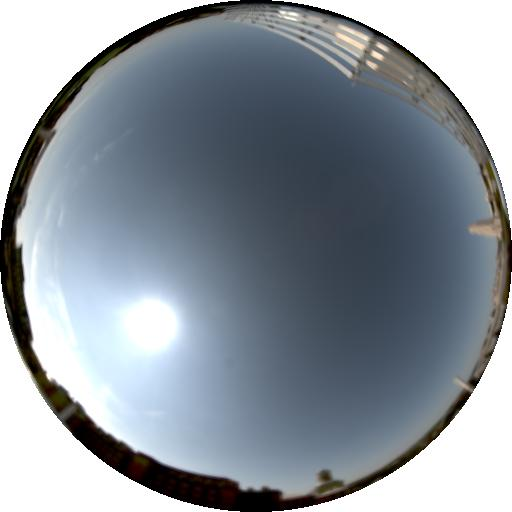
\includegraphics[width=\customwidth]{./figures/database/20130824_110040.jpg} &
    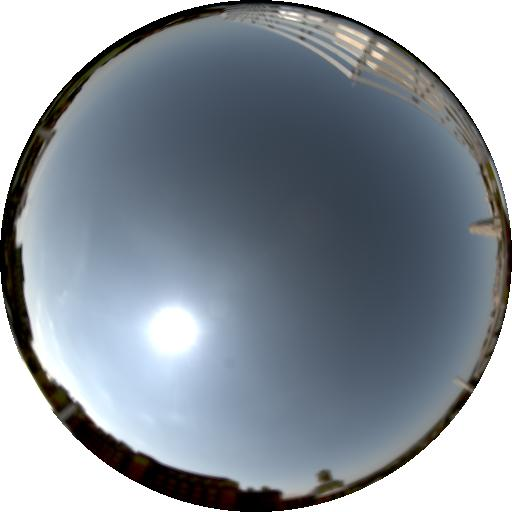
\includegraphics[width=\customwidth]{./figures/database/20130824_113038.jpg} &
    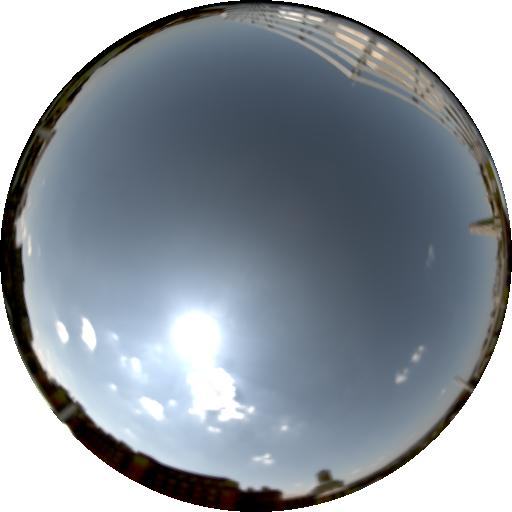
\includegraphics[width=\customwidth]{./figures/database/20130824_120033.jpg} &
    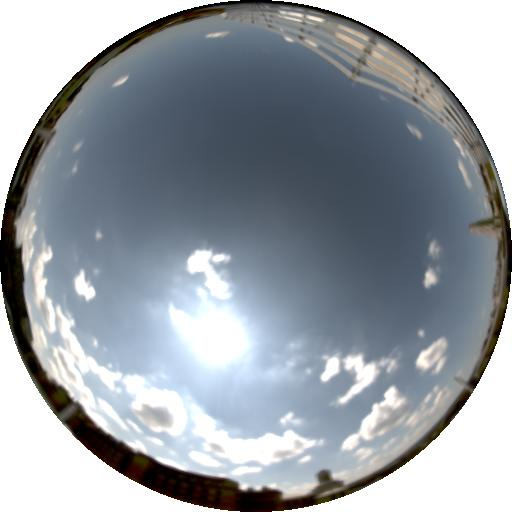
\includegraphics[width=\customwidth]{./figures/database/20130824_123024.jpg} &
    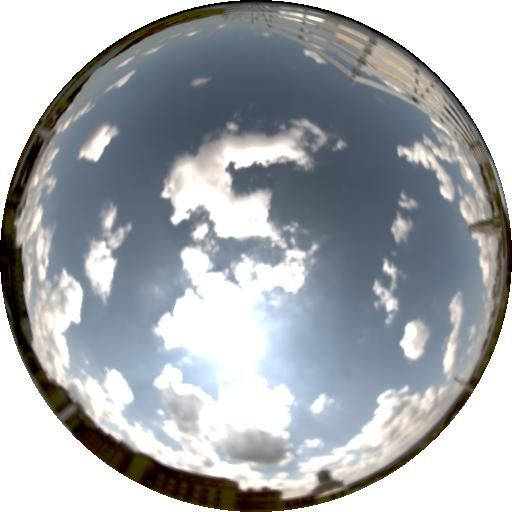
\includegraphics[width=\customwidth]{./figures/database/20130824_130014.jpg} &
    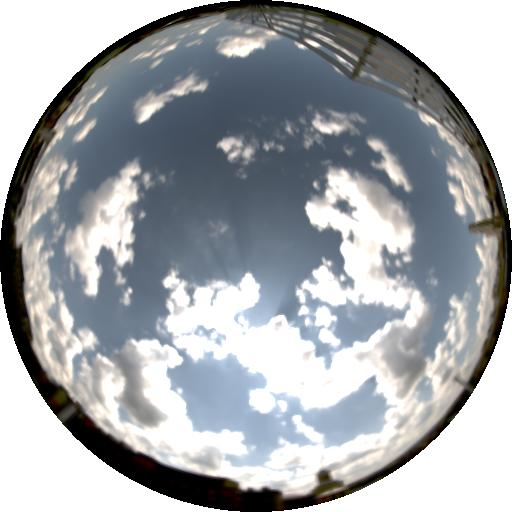
\includegraphics[width=\customwidth]{./figures/database/20130824_133006.jpg} &
    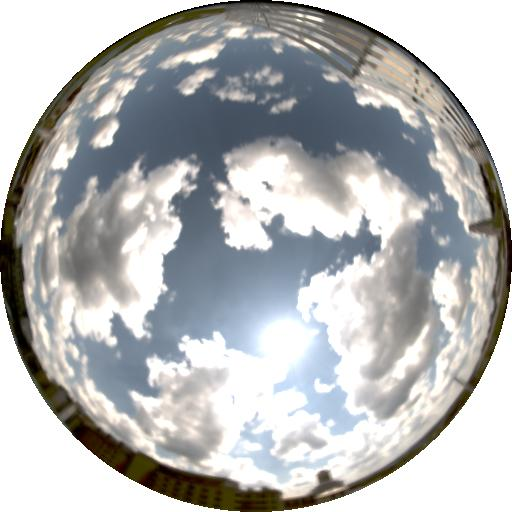
\includegraphics[width=\customwidth]{./figures/database/20130824_140002.jpg} &
    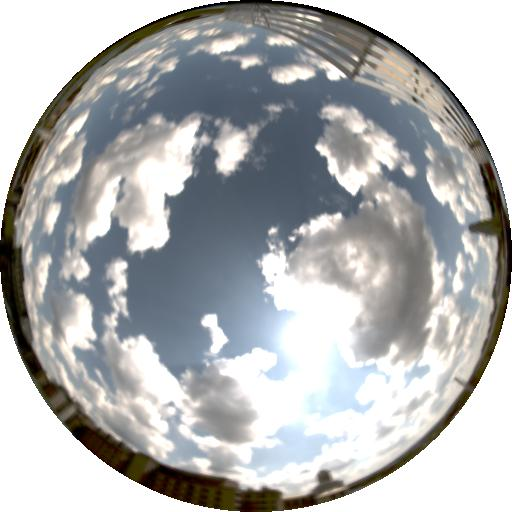
\includegraphics[width=\customwidth]{./figures/database/20130824_142960.jpg} &
    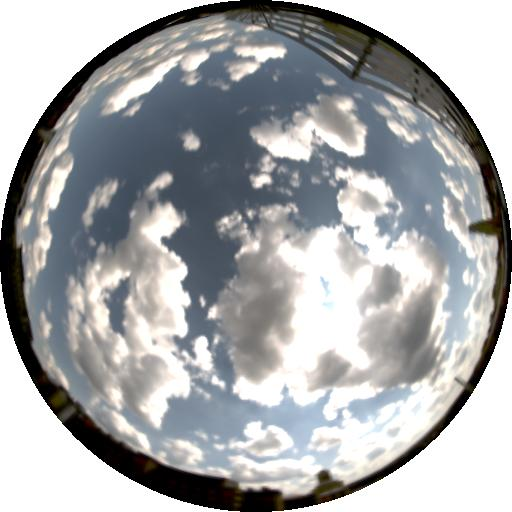
\includegraphics[width=\customwidth]{./figures/database/20130824_145957.jpg} &
    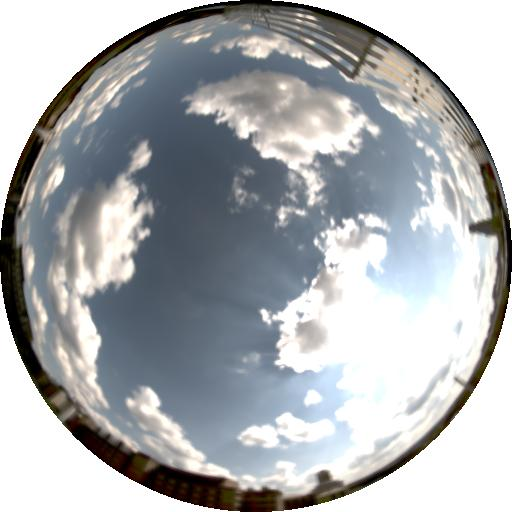
\includegraphics[width=\customwidth]{./figures/database/20130824_152946.jpg} &
    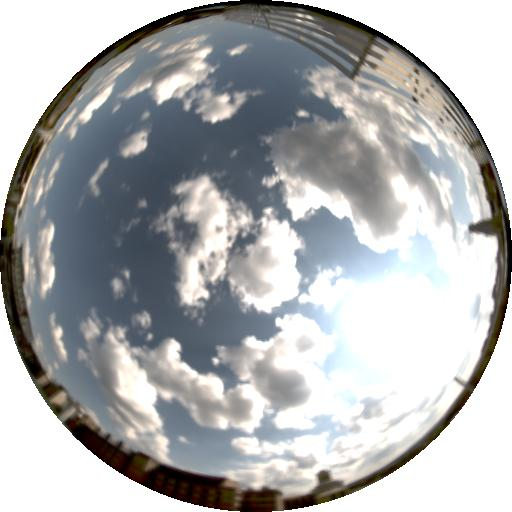
\includegraphics[width=\customwidth]{./figures/database/20130824_155938.jpg} &
    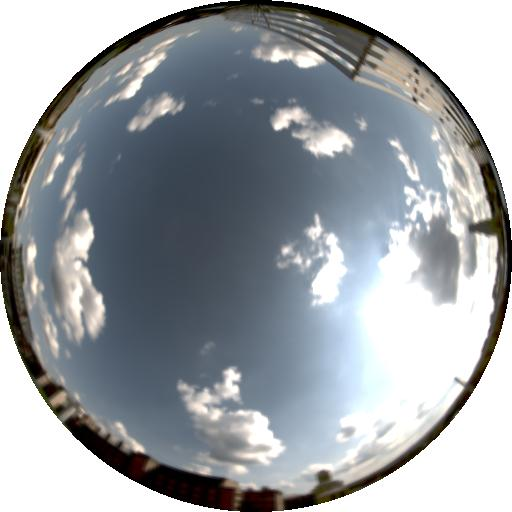
\includegraphics[width=\customwidth]{./figures/database/20130824_162933.jpg}
    \\
    \begin{sideways}\begin{minipage}{\customwidth}\centering \scriptsize 11/06/2013 \\ mixed \vspace{5pt} \end{minipage}\end{sideways} &
    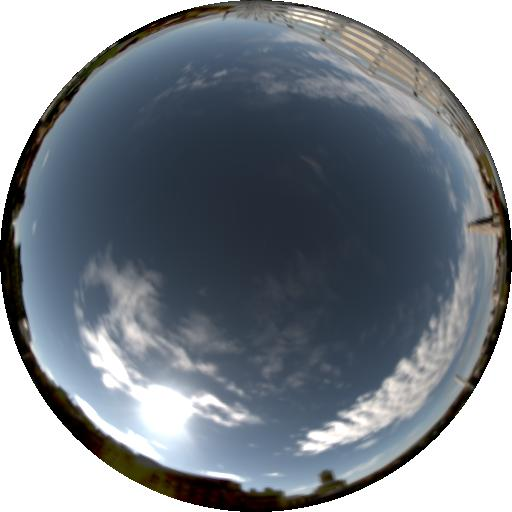
\includegraphics[width=\customwidth]{./figures/database/20131106_110951.jpg} &
    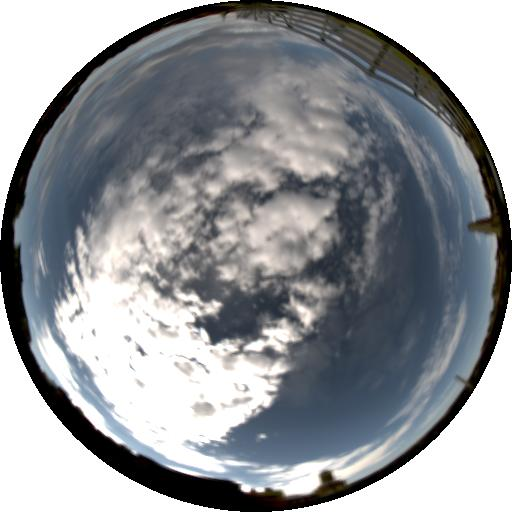
\includegraphics[width=\customwidth]{./figures/database/20131106_112948.jpg} &
    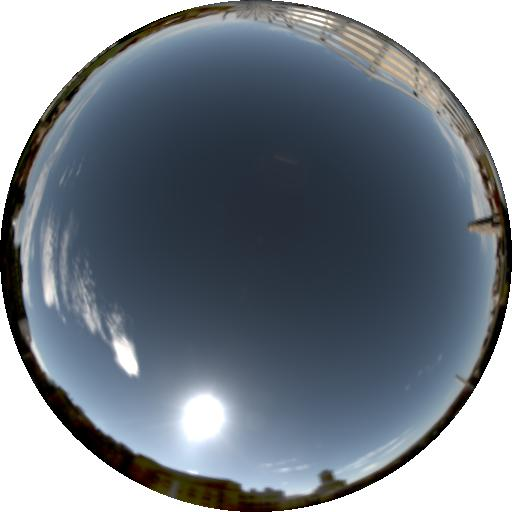
\includegraphics[width=\customwidth]{./figures/database/20131106_115943.jpg} &
    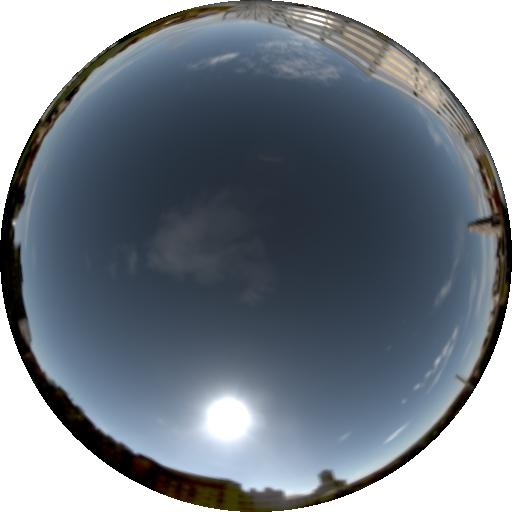
\includegraphics[width=\customwidth]{./figures/database/20131106_122939.jpg} &
    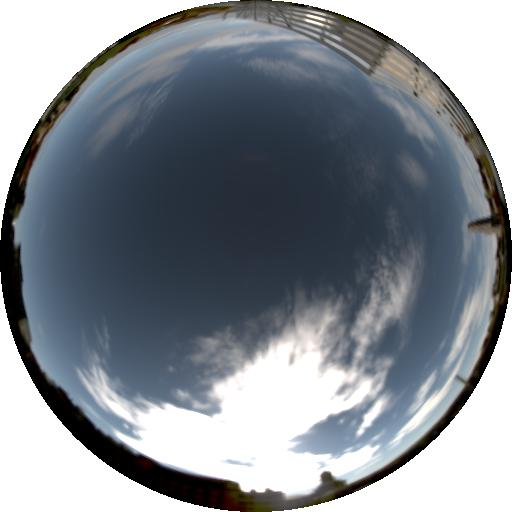
\includegraphics[width=\customwidth]{./figures/database/20131106_125937.jpg} &
    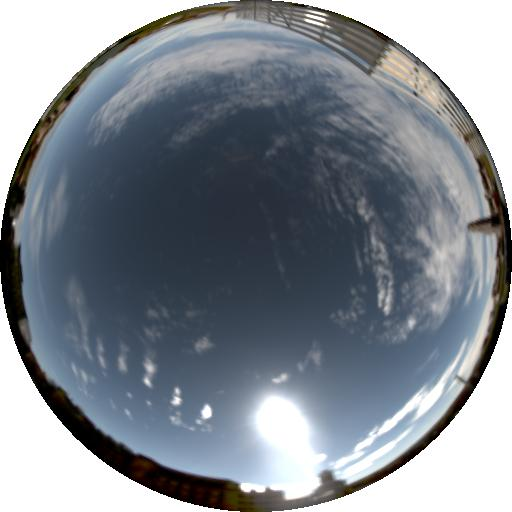
\includegraphics[width=\customwidth]{./figures/database/20131106_132936.jpg} &
    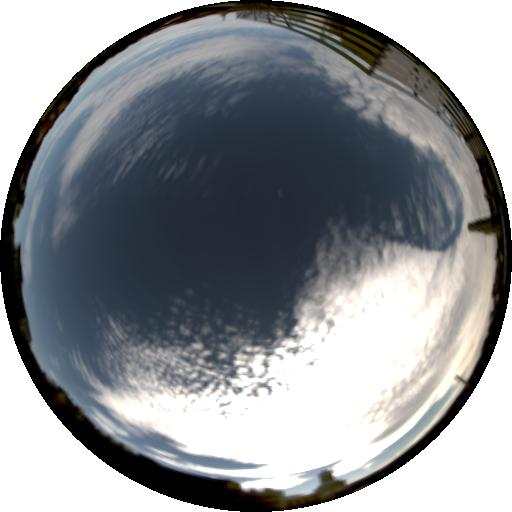
\includegraphics[width=\customwidth]{./figures/database/20131106_135932.jpg} &
    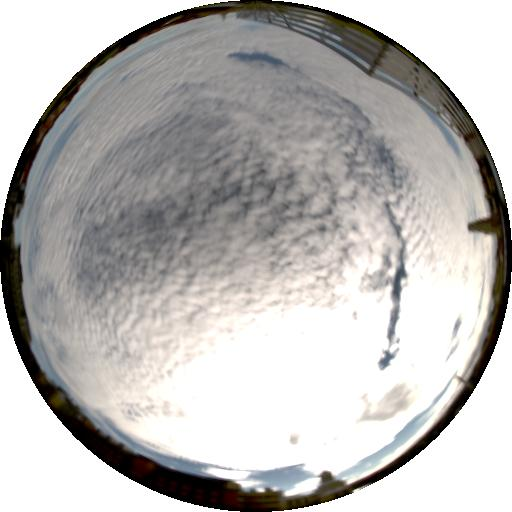
\includegraphics[width=\customwidth]{./figures/database/20131106_142922.jpg} &
    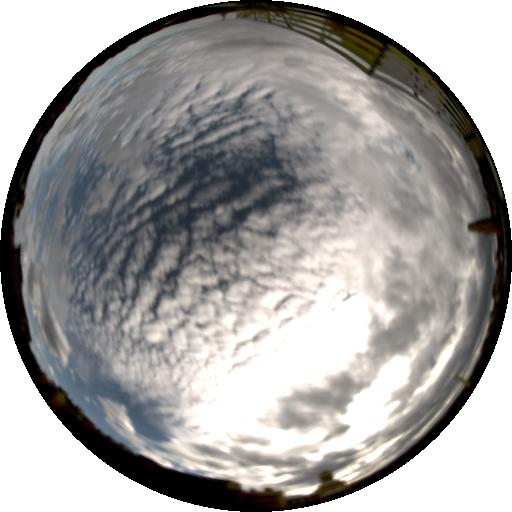
\includegraphics[width=\customwidth]{./figures/database/20131106_145915.jpg} &
    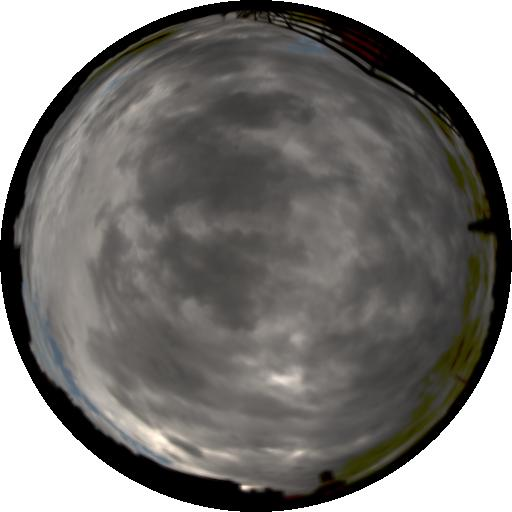
\includegraphics[width=\customwidth]{./figures/database/20131106_152913.jpg} &
    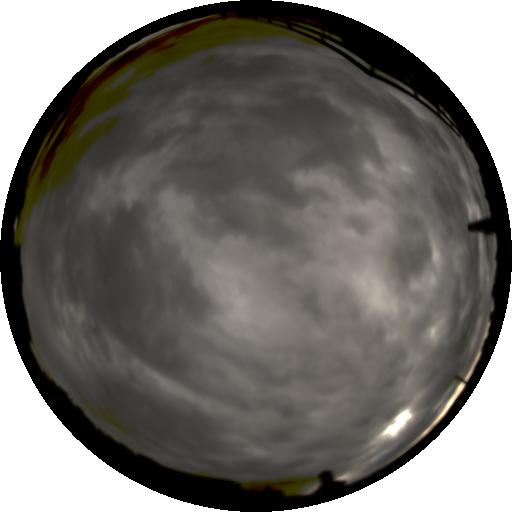
\includegraphics[width=\customwidth]{./figures/database/20131106_155906.jpg} &
    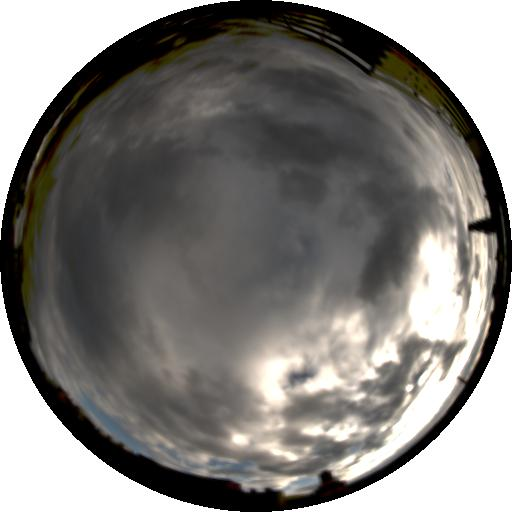
\includegraphics[width=\customwidth]{./figures/database/20131106_163057.jpg}
    \\
    \begin{sideways}\begin{minipage}{\customwidth}\centering \scriptsize 11/08/2014 \\ heavy clds.\vspace{5pt} \end{minipage}\end{sideways} &
    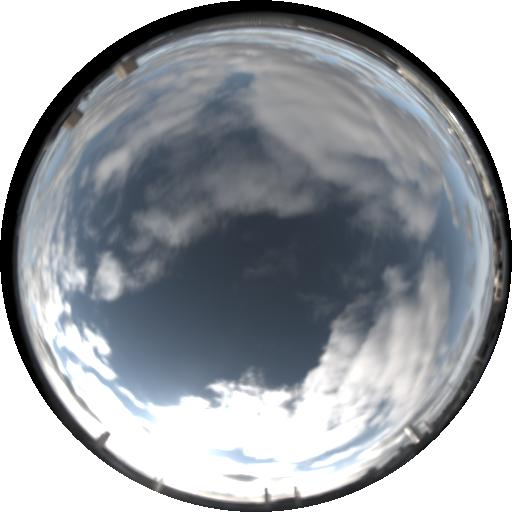
\includegraphics[width=\customwidth]{./figures/database/20141108_110025.jpg} &
    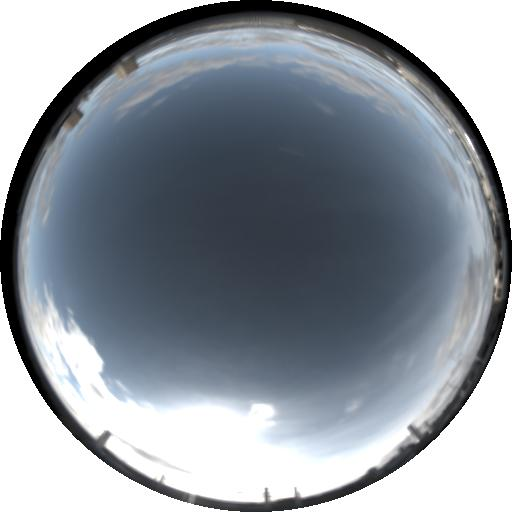
\includegraphics[width=\customwidth]{./figures/database/20141108_113025.jpg} &
    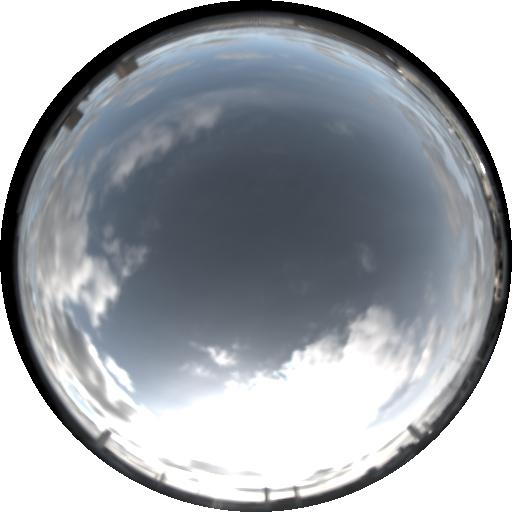
\includegraphics[width=\customwidth]{./figures/database/20141108_120025.jpg} &
    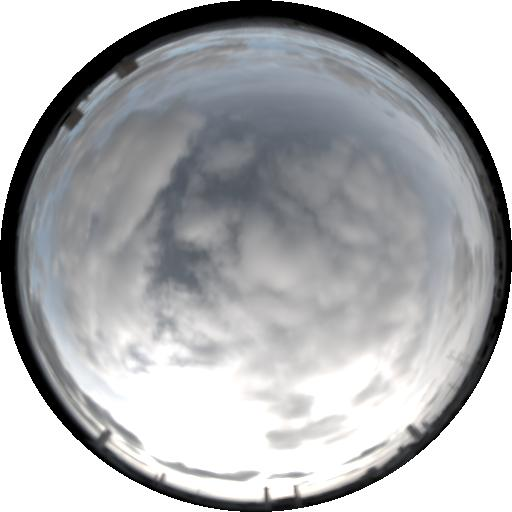
\includegraphics[width=\customwidth]{./figures/database/20141108_123025.jpg} &
    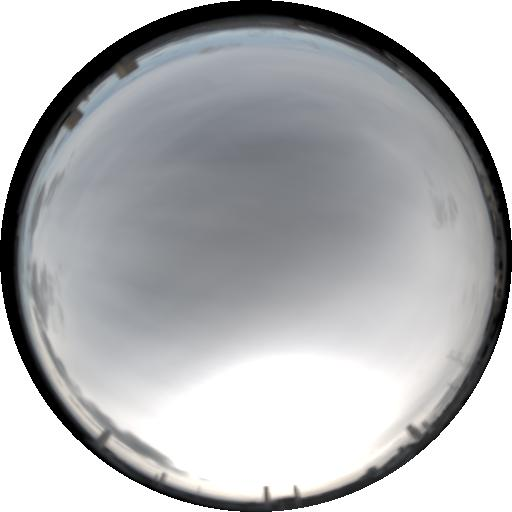
\includegraphics[width=\customwidth]{./figures/database/20141108_130025.jpg} &
    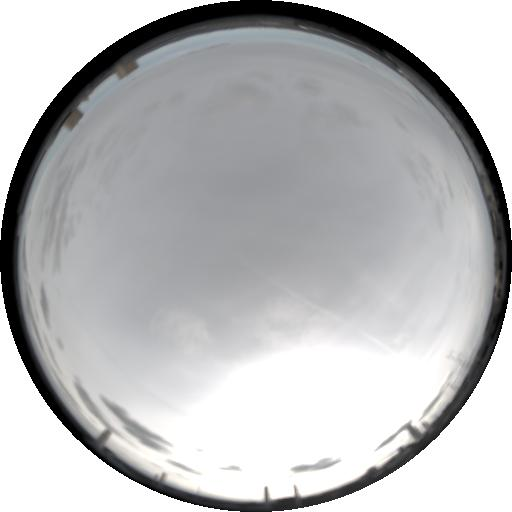
\includegraphics[width=\customwidth]{./figures/database/20141108_133025.jpg} &
    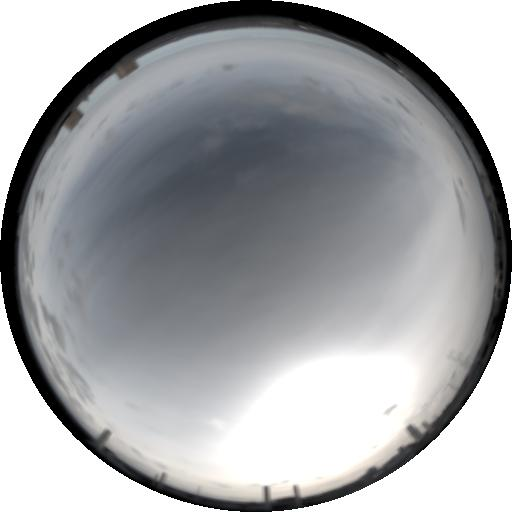
\includegraphics[width=\customwidth]{./figures/database/20141108_140025.jpg} &
    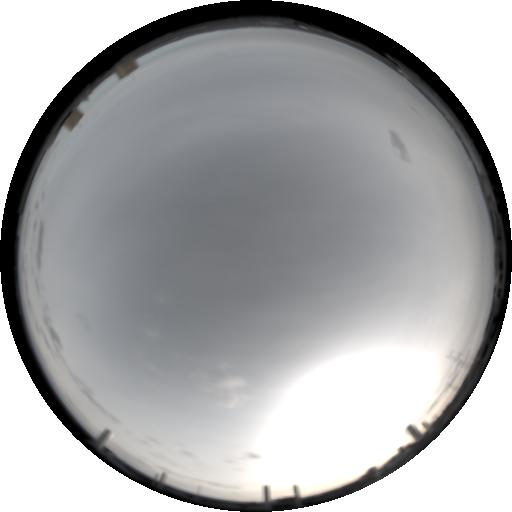
\includegraphics[width=\customwidth]{./figures/database/20141108_143025.jpg} &
    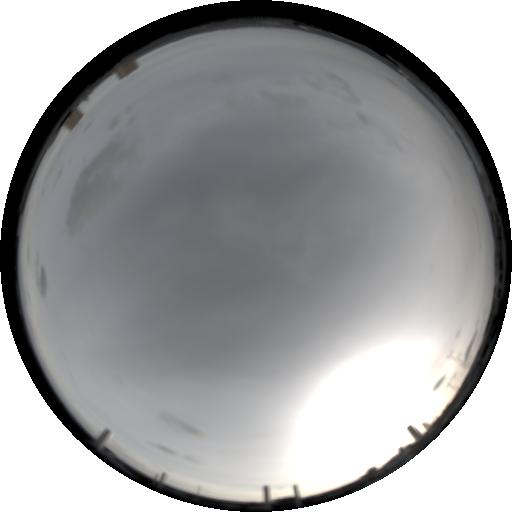
\includegraphics[width=\customwidth]{./figures/database/20141108_150025.jpg} &
    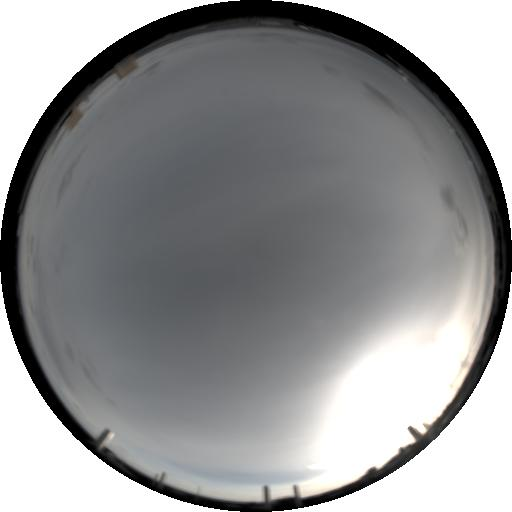
\includegraphics[width=\customwidth]{./figures/database/20141108_153025.jpg} &
    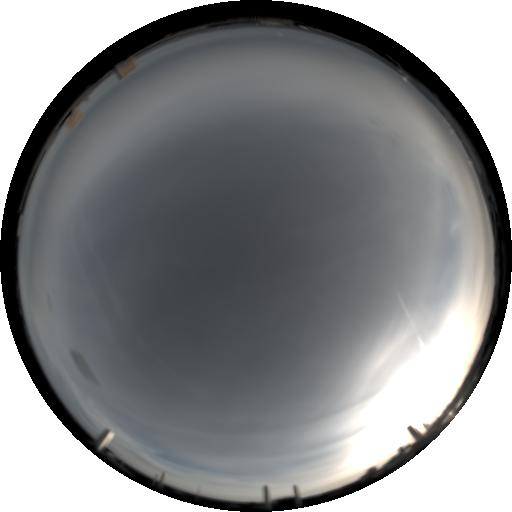
\includegraphics[width=\customwidth]{./figures/database/20141108_160025.jpg} &
    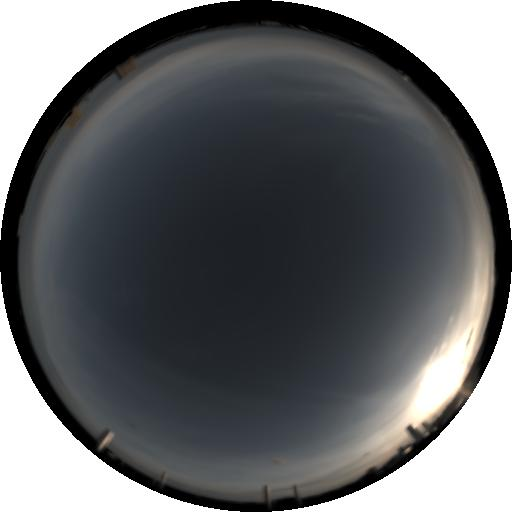
\includegraphics[width=\customwidth]{./figures/database/20141108_163025.jpg}

    \\

    \end{tabular}
    \caption[]{Examples from our dataset of HDR outdoor illumination conditions. In all, our dataset contains 3,800 different illumination conditions, captured from 10:30 until 16:30, during 23 days, spread over ten months and at two geographical locations. Each image is stored in the 32-bit floating point EXR format, and shown tone mapped here for display (with $\gamma = 1.6$). The companion video\footnote{Available at \url{http://vision.gel.ulaval.ca/~jflalonde/projects/outdoorPS/index.html}} shows time-lapse sequences for these sky environment maps.}
    \label{fig:database}
\end{figure}


\begin{figure}
    \centering
    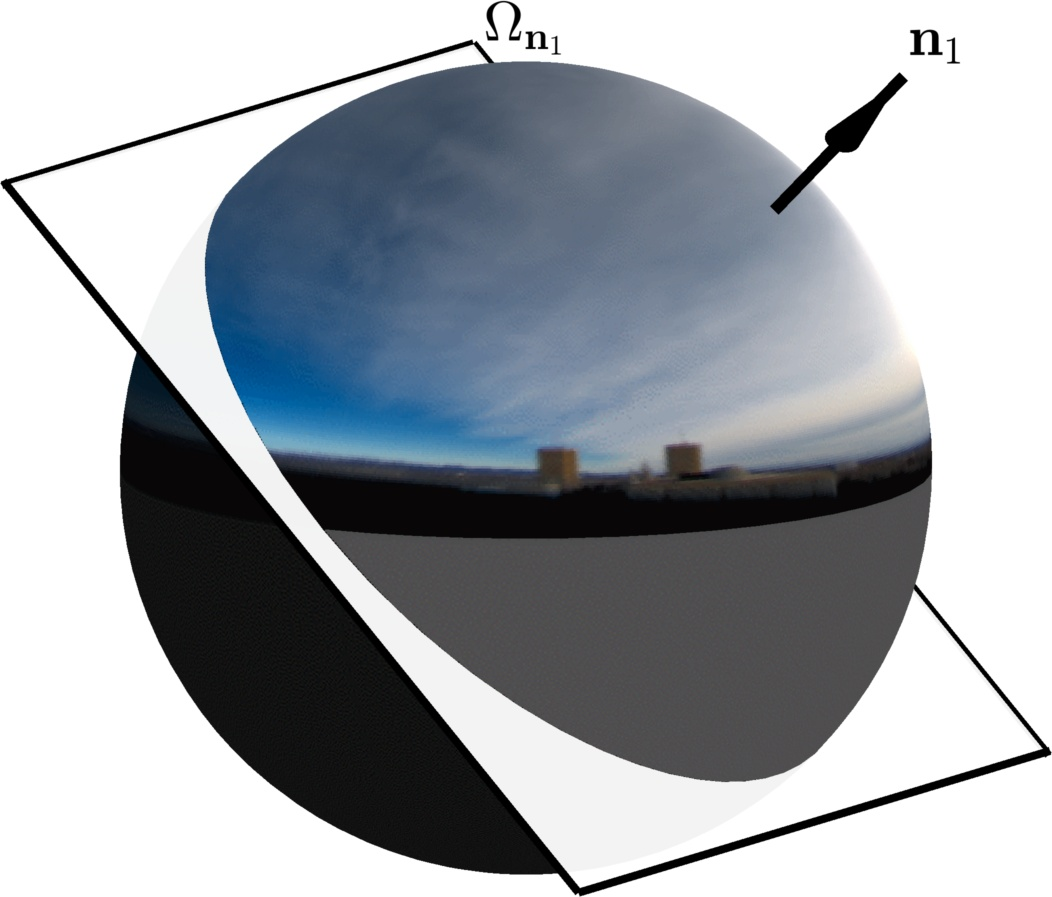
\includegraphics[width=.495\linewidth]{./figures/diagramFig/diagram1.jpg}
    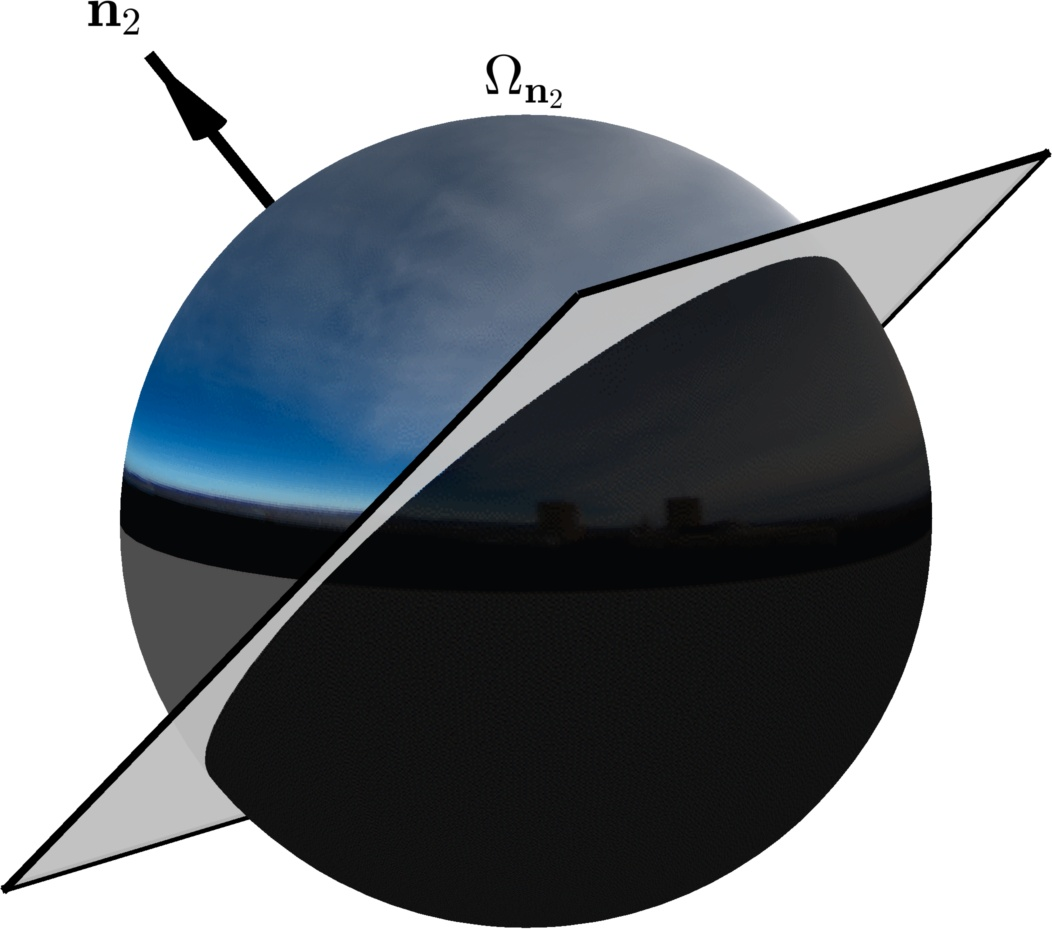
\includegraphics[width=.495\linewidth]{./figures/diagramFig/diagram2.jpg}
    \caption{A normal $\mathbf{n}$ defines an integration domain $\Omega_{\mathbf{n}}$ equivalent to a hemisphere on the entire spherical environment map. Only light emanating from this hemisphere contribute to the shading on that patch. Therefore, patches with different normals are lit differently even if the environment map is the same.}
    \label{fig:normal-diagram}
\end{figure}

This image formation model is then discretized as,
%
\begin{equation}
b_t = \frac{\rho}{\pi}\sum_{\boldomega_j \in \Omega_{\bf n}} \widehat{L}_t(\boldomega_j) \langle \boldomega_j, {\bf n} \rangle\,,
\label{eqn:imageformation-discrete}
\end{equation}
%
with $\widehat{L}_t(\boldomega_j) = L_t(\boldomega_j)\Delta\omega_j$ representing the environment map weighted by the solid angle $\Delta\omega_j$ spanned by pixel $j$ ($\Delta\omega_j$, $\forall j$, are normalized as to sum to $2\pi$). Eq.~$\eqref{eqn:imageformation-discrete}$ can be further summarized into the equivalent form
%
\begin{equation}
b_t = {\bf \bar l}_t^T \mathbf{x}
\label{eqn:imageformation-simplified}
\end{equation}
where ${\bf x} = \rho {\bf n}$ is the albedo-scaled normal vector and
\begin{equation}
{\bf \bar l}_t = \frac{1}{\pi} \sum_{\boldomega_j \in \Omega_{\bf n}} \widehat{L}_t(\boldomega_j) \boldomega_j \in \mathbb{R}^3
\label{eqn:mean-light}
\end{equation}
is interpreted as the {\em mean light vector} for the environment map at a time $t$.

Given multiple images taken at times $t \in \{1,2,\ldots,T\}$, we collect all photometric constraints for patch ${\bf x}$ to obtain:
\begin{equation}
\mathbf{b} =
\begin{bmatrix}
 b_1 \\ b_2 \\ \vdots \\ b_T
\end{bmatrix}
=
\begin{bmatrix}
 {\bf \bar l}_1^T \\ {\bf \bar l}_2^T \\ \vdots \\ {\bf \bar l}_T^T
\end{bmatrix}
{\bf x} = \mathbf{L} \mathbf{x} \,.
\label{eqn:matrix-form}
\end{equation}
With~\eqref{eqn:matrix-form}, this model of natural environmental illumination becomes quite similar to a model with a distant point light source, the well-known case in PS. However, note that each ${\bf \bar l}_t$ in ${\bf L}$ is a function of $\Omega_{\bf n}$ and, thus, of ${\bf n}$.

Most importantly, in outdoor PS, a well-defined solution ${\bf x}$ may exist even if the relative sun motion is nearly planar during a certain time interval. Instead of relying solely on sun direction, now, the solution requires non-coplanar mean light vectors ${\bf \bar l}_t$, which are determined by a comprehensive set of natural illumination factors.

\section{Modeling uncertainty}

From~\eqref{eqn:matrix-form}, the least-squares solution ${\bf x} = ({\bf L}^T{\bf L})^{-1}{\bf L}^T{\bf b}$ of outdoor PS is clearly affected by the condition number of ${\bf L}$. Thus, we next characterize how well the solution ${\bf x}$ is constrained by natural, outdoor illumination within a given time interval (\eg, one day)---which is encoded by the set of mean light vectors ${\bf \bar l}_t$ in ${\bf L}$ or, equivalently, the set of environment maps $L_t(\cdot)$.

To assess the reliability of a solution ${\bf x}$, we follow standard practice in PS~\cite{klaudiny-prl-14,sun-ivc-07} and consider image measurements corrupted by zero-mean Gaussian noise with equal variance $\sigma^2$ (as least squares estimation is only optimal for this practical, most common noise model). Thus, ${\bf b}$ in~\eqref{eqn:matrix-form} follows a normal distribution:
%
\begin{equation}
{\bf b} \sim \mathcal{N}\left( \boldmu_b, \sigma^2 {\bf I} \right)\,,
\end{equation}
%
where $\boldmu_b$ has the (unknown) uncorrupted pixel values.

Since the desired least-squares solution for the albedo-scaled normal, ${\bf x} = \left({\bf L}^T{\bf L}\right)^{-1}{\bf L}^T{\bf b}$, is a linear transformation of a Gaussian random vector, it is easy to show that
%
\begin{equation}
{\bf x} \sim \mathcal{N} \left( \boldmu_x, \sigma^2({\bf L}^T{\bf L})^{-1} \right)\,,
\end{equation}
where $\boldmu_x = \left({\bf L}^T{\bf L}\right)^{-1}{\bf L}^T\boldmu_b$ is the expected value of ${\bf x}$.
Once the albedo of a surface patch is known, we analyze its contribution to the uncertainty in the estimated normal vector, ${\bf n} = \rho^{-1}{\bf x}$, using a similar distribution,
%
\begin{equation}
{\bf n} \sim \mathcal{N} \left( \frac{\boldmu_x}{\rho}, \frac{\sigma^2}{\rho^2}({\bf L}^T{\bf L})^{-1} \right)\,.
\label{eqn:normal-distrib}
\end{equation}

The marginal distributions in~\eqref{eqn:normal-distrib} allow us to derive confidence intervals that indicate the uncertainty in each component of the least squares estimate ${\bf \hat n} = [ \hat n_x \ \hat n_y \ \hat n_z ]^T$ of ${\bf n} = [ n_x \ n_y \ n_z ]^T$. The corresponding $95\%$ confidence interval~\cite{hastie-book-09} is given by
%
\begin{equation}
\hat{\mathbf{n}} \pm \bolddelta \,, \quad \text{with } \delta_k = 1.96 \frac{\sigma\lambda_k}{\rho} \,,
\label{eqn:confidence-xyz}
\end{equation}
%
where $\lambda_k$ is the square root of the $k$th element on the diagonal of $({\bf L}^T{\bf L})^{-1}$. As expected, the sensor-dependent noise level $\sigma$ is not the only factor that determines uncertainty. The gain factor $\lambda_k/\rho$ in \eqref{eqn:confidence-xyz} reveals how outdoor illumination (the conditioning of ${\bf L}$) and albedo can amplify the effect of noise on the solution ${\bf \hat n}$. The lower the albedo $\rho$ is, the larger is the variance in the obtained estimate $\bf \hat n$ (as less light is reflected towards the camera). Our goal is then to answer the remaining question: how do natural changes in outdoor illumination affect this gain factor ($\lambda_k$) and, therefore, uncertainty?

\section{An intuitive measure of uncertainty}
\label{subsec:measure_uncertainty}

To provide a measure of uncertainty that is more intuitive than~\eqref{eqn:confidence-xyz}, we consider angular distances in degrees,
%
\begin{equation}
\theta^\pm = \cos^{-1}(\mathbf{n}^T{\bf \hat n}^\pm)\,,
\quad \text{where }
{\bf \hat n}^\pm = \frac{{\bf \hat n} \pm \bolddelta}{\lVert{\bf \hat n} \pm \bolddelta \rVert}\,.
\label{eqn:angular-dist}
\end{equation}
%
The uncertainty in the estimate of ${\bf n}$ is then summarized in a single confidence interval, in degrees,
%
\begin{equation}
\mathcal{C}_{\bf n} = [ \ 0, \ \max (\theta^\pm) \ ]\,,
\label{eqn:confidence-degrees}
\end{equation}
which indicates the expected accuracy of the estimated surface orientation ${\bf \hat n}$.

Note that the condition number, determinant, and trace of matrix $(\mathbf{L}^T\mathbf{L})^{-1}$ can also be used as measures of total variance in the estimated solutions---as done in~\cite{sun-ivc-07}---to find the optimal location of point light sources in PS. These measures are closely related to the rank of matrix $\mathbf{L}$, which must be three for a solution to exist; that is, $\mathbf{L}^T\mathbf{L}$ must be nonsingular. In practice, this matrix is always full-rank, although it is often poorly conditioned~\cite{shen-pg-14}. In the remaining sections, we consider confidence intervals $\mathcal{C}_{\bf n}$ in degrees, as they provide a more intuitive measure of uncertainty in the obtained solutions. Finally, in~\eqref{eqn:angular-dist}, the normalization of ${\bf \hat n}^\pm$ to unit length reflects the fact that part of the estimation error is propagated to the estimated albedo $\rho$ (\ie, the length of the computed least-squares solution vector ${\bf x}$). In this chapter, we focus on analyzing our ability to recover geometry and will assume that the albedo is constant and known.

\subsection{Analyzing the outdoor lighting dataset}
\label{sec:iccp15-datasetanalysis}

% context, need, task, object, conclusions, perspective
Now that we are equipped with a tool to characterize the stability of surface normal estimation in outdoor PS, we proceed to apply it to all 23 days from our dataset (sec.~\ref{sec:hdrdb}) in order to determine the conditions in which surface normals can accurately be reconstructed. We first describe how the confidence intervals $\mathcal{C}_{\bf n}$ are computed and visualized, then analyze the effect of two important characteristics of outdoor lighting: the degree of cloud coverage in sec.~\ref{sec:cloud-cover-results}, and the sun elevation in sec.~\ref{sec:sun-elevation-results}.

\begin{figure}[t]
    \centering
    \begin{minipage}{.5\linewidth}
    \begin{sideways}\begin{minipage}{.4\linewidth}\centering \scriptsize 08/24/2013 \\ 85\% sun visibility \vspace{5pt} \end{minipage}\end{sideways}
    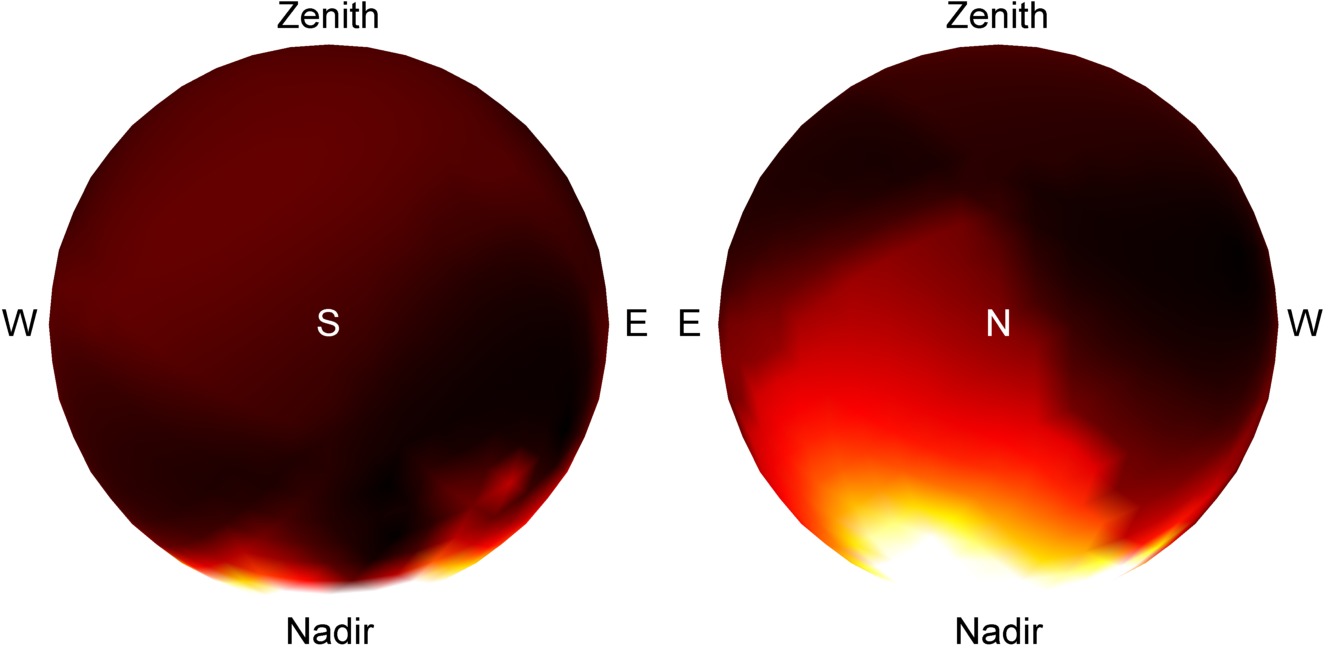
\includegraphics[width=.9\linewidth]{./figures/confidenceIntervals/20130824_10pm.png} \\
    \vspace{-.8em} \noindent\rule{\linewidth}{0.1pt}
    \begin{sideways}\begin{minipage}{.4\linewidth}\centering \scriptsize 11/06/2013 \\ 41\% sun visibility \vspace{5pt} \end{minipage}\end{sideways}
    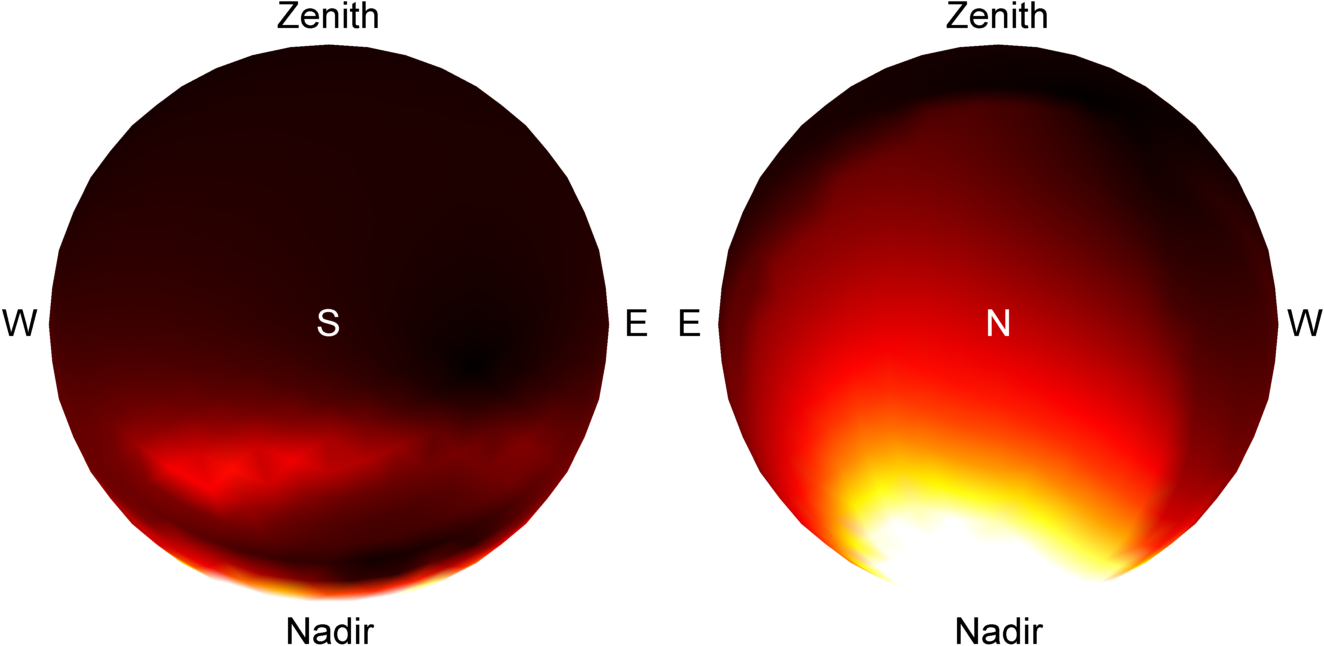
\includegraphics[width=.9\linewidth]{./figures/confidenceIntervals/20131106_10pm.png} \\
    \vspace{-.8em} \noindent\rule{\linewidth}{0.1pt}
    \begin{sideways}\begin{minipage}{.4\linewidth}\centering \scriptsize 11/08/2014 \\ 16\% sun visibility \vspace{5pt} \end{minipage}\end{sideways}
    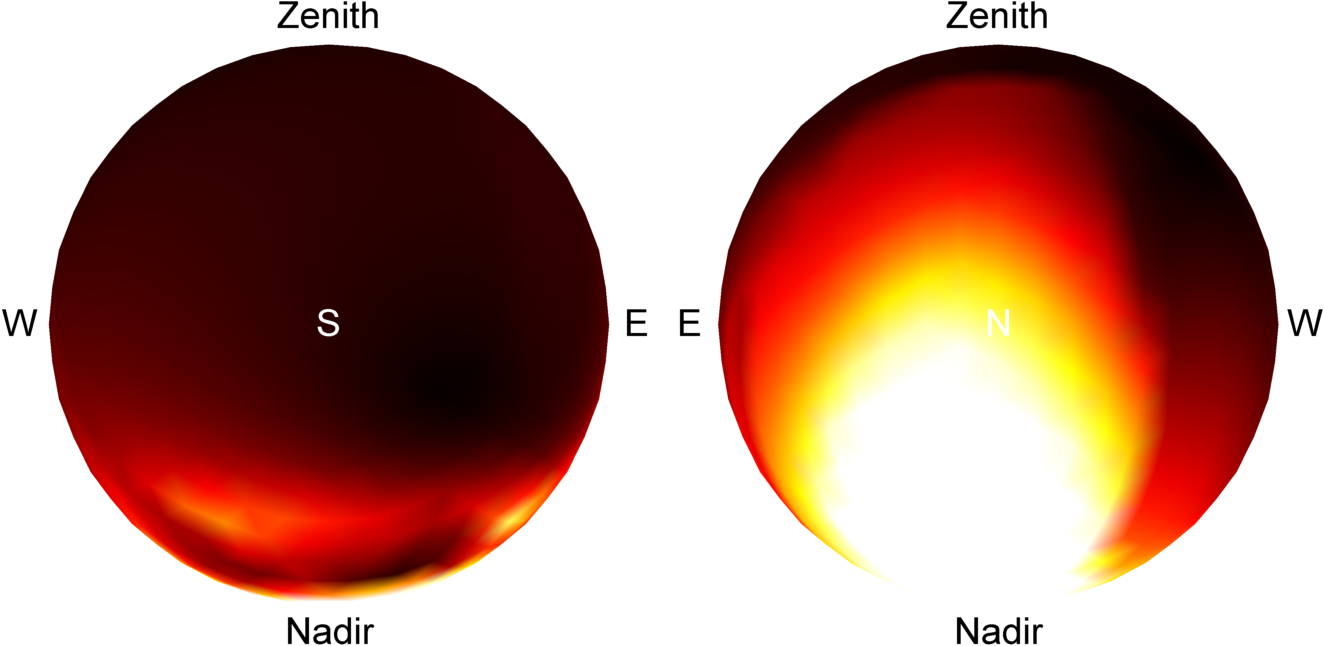
\includegraphics[width=.9\linewidth]{./figures/confidenceIntervals/20141108_10pm.png} \\
    \end{minipage}
    \vspace{3mm}
    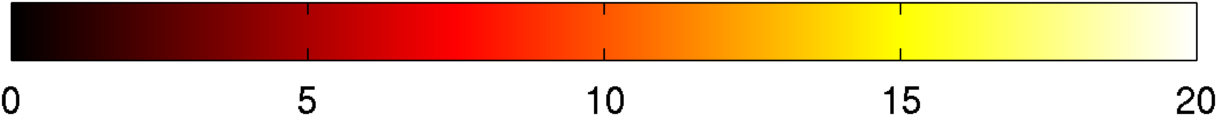
\includegraphics[width=.51\linewidth]{./figures/confidenceIntervals/colorbar.png}
    \caption{Uncertainty in normal estimation with $\sigma=1\%$ is indicated by 95\% confidence intervals (in degrees), as a function of ground-truth surface normal. Results are shown for three different days in our dataset (same days as in fig.~\ref{fig:database}). The plots show the full sphere of normals from two different viewpoints: South (left), and North (right). Cardinal directions are shown for reference. The color-coding is indicated below the plots. See companion video for an animated version of these plots.}
    \label{fig:confidence-intervals}
\end{figure}

\begin{figure*}[t]
    \centering
    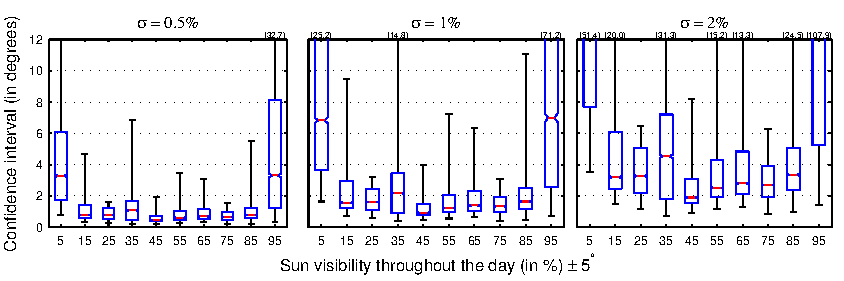
\includegraphics[width=.99\linewidth]{./figures/confidenceIntervals/sunVisibilityPlot-topHemisphere.pdf}
    \vspace{-2mm}
    \caption{Median confidence interval of normal estimates (red line) as a function of mean sun visibility over the course of the day for various values of $\sigma$. Our analysis predicts that normal reconstruction errors will likely be high if the sky is completely overcast (low sun visibility), or completely clear (high sun visibility). Good results can thus be expected in partially cloudy conditions, as shown in fig.~\ref{fig:cloud-cover}. The lower (upper) edge of each blue box indicates the 25th (75th) percentile. Statistics are computed only on normals pointing upwards to lessen ground effects.}
    \label{fig:cloud-cover-plot}
\end{figure*}


\section{Computing the stability of outdoor PS}
\label{iccp-computingstability}

We aim to apply the stability analysis of sec.~\ref{sec:ch1_analysis} on all 23 days from our dataset, and on all possible normal directions. To do so, we consider each day independently, and first sample directions on the sphere by subdividing an icosahedron three times, yielding a set of 642 potential orientations $\mathcal{N} = \{\mathbf{n}_1, ..., \mathbf{n}_{642} \}$. Then, for each $\mathbf{n}_j \in \mathcal{N}$, we build the illumination matrix $\mathbf{L}$ in~\eqref{eqn:matrix-form}, given all 6 hours of data for that day. Finally, the 95\% confidence interval $\mathcal{C}_{\mathbf{n}_j}$ is computed using~\eqref{eqn:confidence-degrees}, indicating the uncertainty (possible reconstruction error) for that normal---the higher the interval, the less stable the solution.

To compute $\mathcal{C}_{\mathbf{n}_j}$, values for the noise level $\sigma$ and the surface albedo $\rho$ from \eqref{eqn:confidence-xyz} must be chosen. For the albedo, we will consider the best case with $\rho=1$. To set $\sigma$, we first render noise-less pixel values $\mathbf{b}_j$ using the (ground-truth) normal ${\bf n}_j$ and~\eqref{eqn:matrix-form}, with ${\bf L}$ including our entire collection of environment maps. All figures have been generated with $\sigma$ set at $1\%$ of the 95th percentile value of the resulting $\mathbf{b}_j$, unless otherwise stated. This particular value is chosen to yield a small, yet non-negligible, level of noise that is similar to that in previous work~\cite{klaudiny-prl-14}. The values of $\rho$ and $\sigma$ are kept constant in order to focus solely on the influence of lighting conditions, but could be set to match particular experimental conditions if needed.

Fig.~\ref{fig:confidence-intervals} shows the result of such an analysis on the three days of fig.~\ref{fig:database}. For each day, two sides of the sphere of normal directions are shown: seen from the South (left), and from the North (right). The spheres are color-coded according to the confidence interval $\mathcal{C}_\mathbf{n}$ for each normal direction. Note that vertex interpolation is used to display full spheres, but valid data is available only at vertices (thus the staircase effect in some plots).

At first glance, we notice that normals pointing down (towards Nadir) consistently have high confidence intervals, irrespective of the illumination conditions. The stability of outdoor PS on these normals is thus expected to be low. This behavior concords with expectation: normals pointing down define integration domains $\Omega_{\mathbf{n}}$ (see fig.~\ref{fig:normal-diagram}) which mostly include the ground, whose intensity does not vary spatially throughout the day. Another interesting observation from fig.~\ref{fig:confidence-intervals} is that the same normal exhibits different confidence intervals depending on the day. This raises the question: what is the relation between outdoor illumination conditions and uncertainty in the recovered surface normal?


\section{Influence of cloud cover}
\label{sec:cloud-cover-results}

It is already apparent from fig.~\ref{fig:confidence-intervals} that cloud coverage has an effect on the uncertainty of normal reconstruction, since an overcast day (last row) clearly does not behave the same way as a day with light clouds (top row). Here, we present a more systematic analysis of the influence of cloud coverage. To control for the effect of the sun elevation (which will be explored in sec.~\ref{sec:sun-elevation-results}), the analysis is performed on days with similar sun elevations by keeping only the skies captured in October and November.

We approximate cloud coverage by computing the fraction of time that the sun is visible, \ie, that it fully shines on the scene, for a given day. To do so, we simply find the brightest spot in a sky image, and determine that the sun shines on the scene if the intensity of the brightest pixel is greater than $20\%$ of the maximum sun intensity---we determined empirically that this is the point at which the sun is bright enough to start creating cast shadows. Cloud coverage is represented by computing the mean sun visibility for a given day. A value of less than 10--15\% would indicate a mostly overcast sky, while skies are mostly clear with values above 85--90\%.

\begin{figure}[t]
    \centering
    \begin{minipage}{.5\linewidth}
    \begin{sideways}\begin{minipage}{.4\linewidth}\centering \scriptsize Clear (85-100\%)\vspace{5pt} \end{minipage}\end{sideways}
    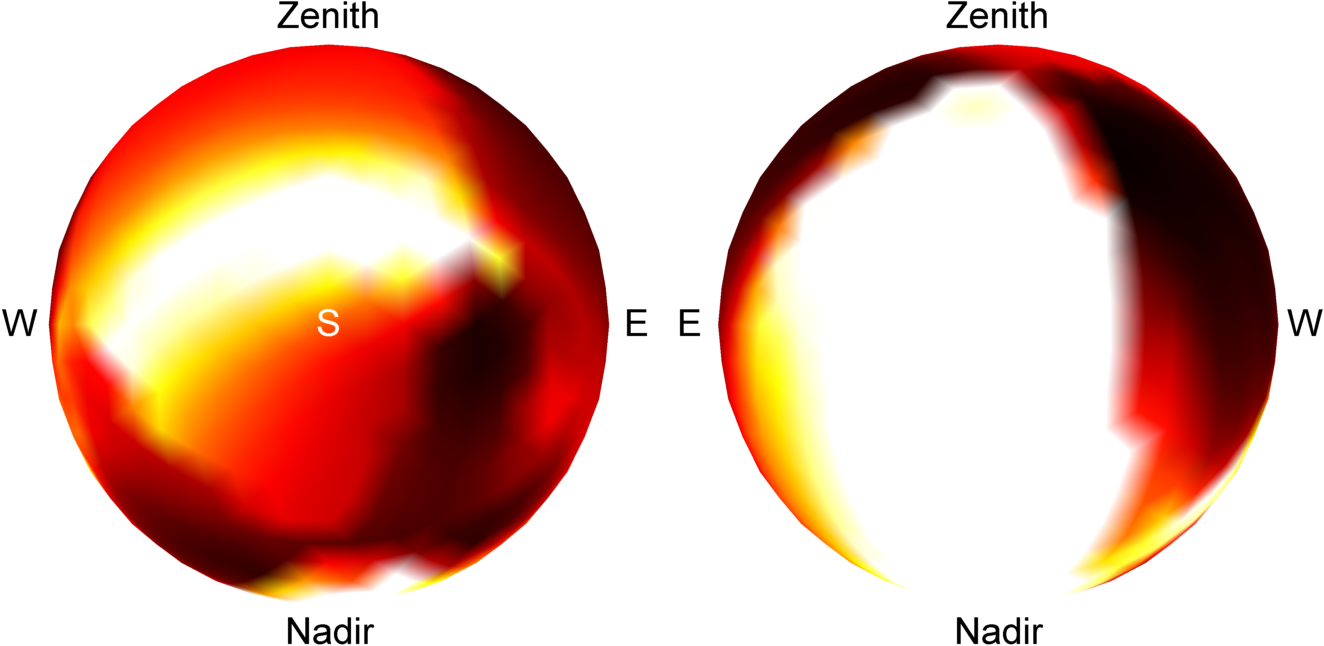
\includegraphics[width=.9\linewidth]{./figures/confidenceIntervals/clear-mean_10pm.png} \\
    \vspace{.4em} \noindent\rule{\linewidth}{0.1pt} \vspace{-.8em}
    \begin{sideways}\begin{minipage}{.4\linewidth}\centering \scriptsize Mixed Clear (50-85\%)\vspace{5pt} \end{minipage}\end{sideways}
    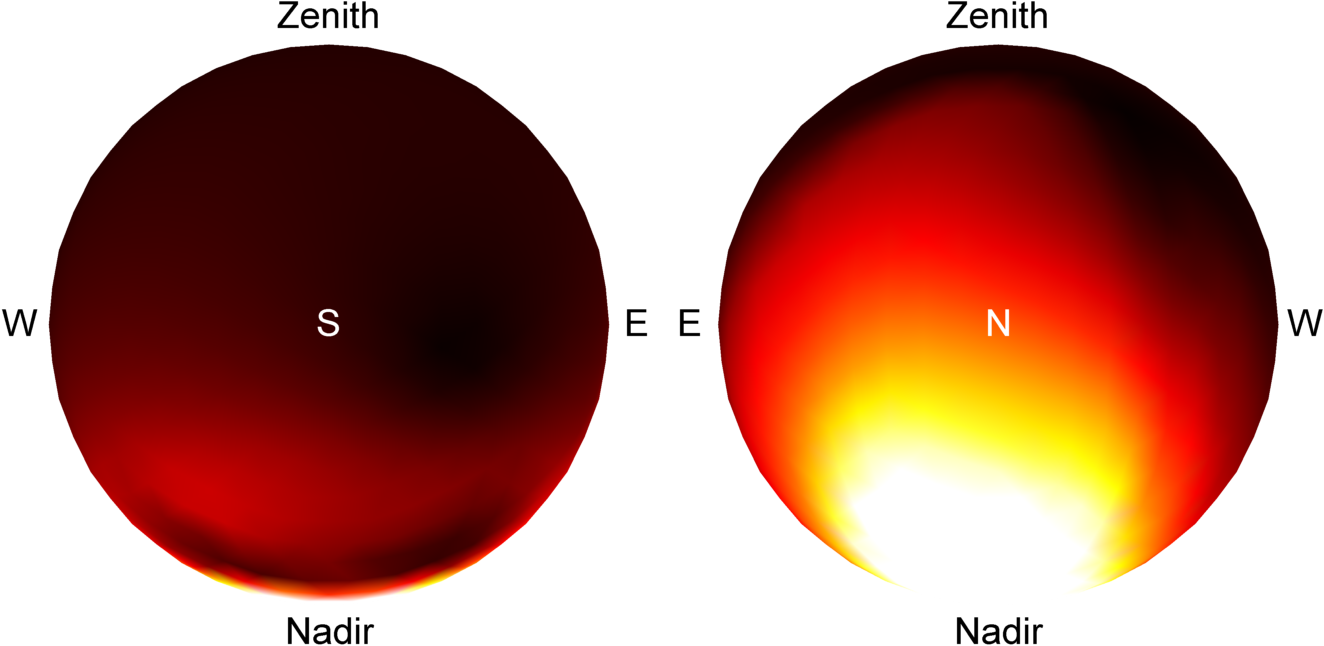
\includegraphics[width=.9\linewidth]{./figures/confidenceIntervals/mixed-clear-mean_10pm.png} \\
    \vspace{.4em} \noindent\rule{\linewidth}{0.1pt} \vspace{-.8em}
    \begin{sideways}\begin{minipage}{.4\linewidth}\centering \scriptsize Mixed Overcast (15-50\%)\vspace{5pt} \end{minipage}\end{sideways}
    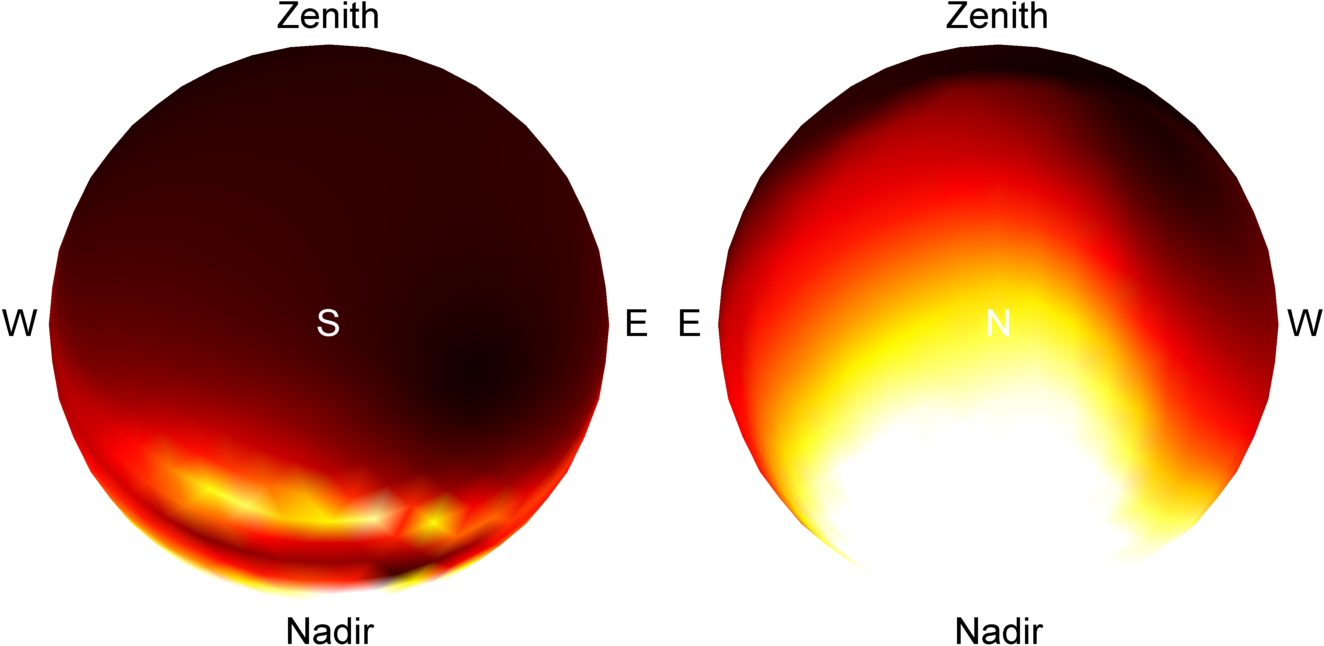
\includegraphics[width=.9\linewidth]{./figures/confidenceIntervals/mixed-overcast-mean_10pm.png} \\
    \vspace{.4em} \noindent\rule{\linewidth}{0.1pt} \vspace{-.8em}
    \begin{sideways}\begin{minipage}{.4\linewidth}\centering \scriptsize Overcast (0-15\%)\vspace{5pt} \end{minipage}\end{sideways}
    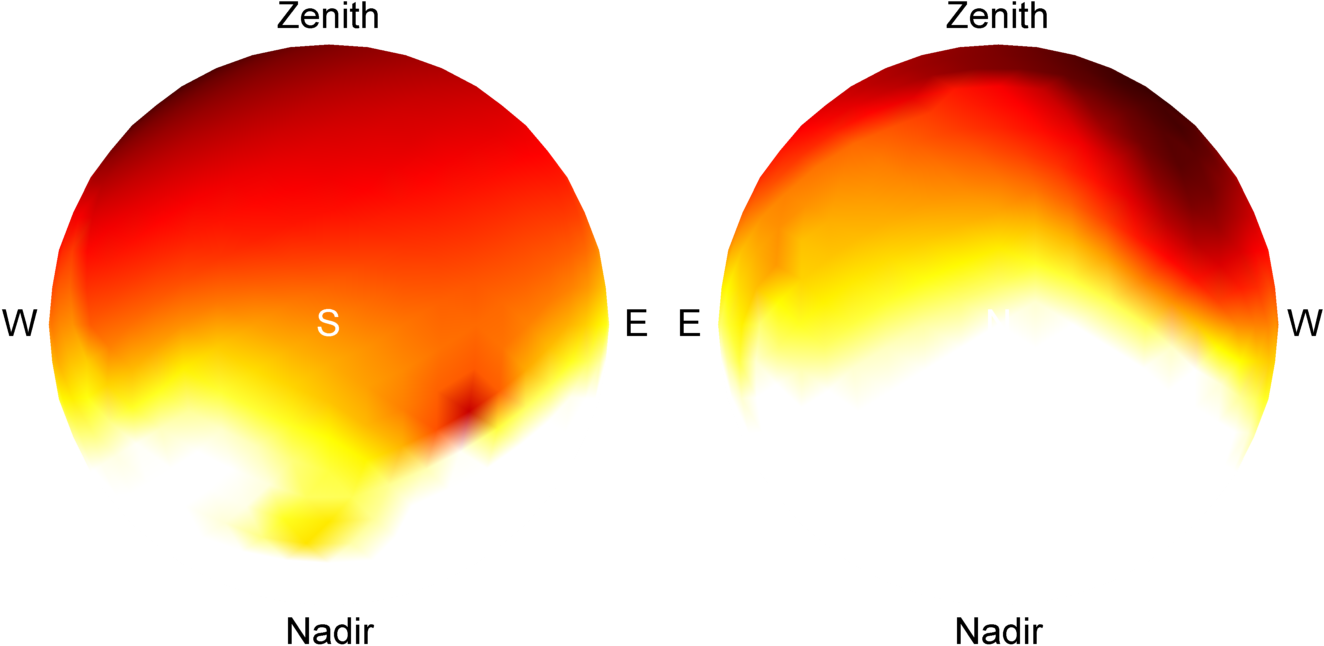
\includegraphics[width=.9\linewidth]{./figures/confidenceIntervals/overcast-mean_10pm.png} \\
    \end{minipage}
    \vspace{3mm}
    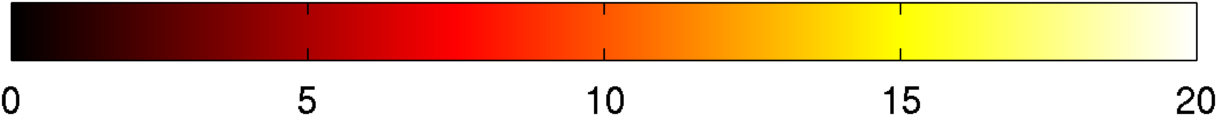
\includegraphics[width=.51\linewidth]{./figures/confidenceIntervals/colorbar.png}
    \caption{Influence of cloud cover on the 95\% confidence intervals with $\sigma=1\%$. Each row shows a different type of sky, based on sun visibility. For example, the top row shows confidence intervals averaged over all days with direct sun visibility in the range 85\%-100\%. The averaged days presented similar sun elevations. As with fig.~\ref{fig:confidence-intervals}, the plots show the full sphere of normals from two different viewpoints: South (left), and North (right).}
    \label{fig:cloud-cover}
\end{figure}

The relation between sun visibility and the confidence interval $\mathcal{C}_\mathbf{n}$ is shown in fig.~\ref{fig:cloud-cover-plot}. Normal reconstruction errors will likely be quite high in two situations: when the sky is completely overcast (low sun visibility), or completely clear (high sun visibility). Interestingly, good reconstruction results are expected for a wide range of cloud coverage conditions, ranging from 10--90\% mean sun visibility.

These results are corroborated by fig.~\ref{fig:cloud-cover}, which shows the confidence intervals themselves on a plot similar to fig.~\ref{fig:confidence-intervals}. Results there are presented by averaging the intervals of skies belonging to four groups: overcast (0--15\%), mixed overcast (15--50\%), mixed clear (50--85\%), and clear (85--100\%) days. Again, high uncertainty results are visible for the two extreme cases of fully overcast and fully clear days, while the remainder indicate more stable solutions.

% TODO: add figure to illustrate this (maybe)?
The improved conditioning in mixed skies is explained by the following key observation: cloud cover shifts the mean light vectors ${\bf \bar l}_t$ towards zenith and away from sun trajectory in the sky. Therefore, even when the sun moves along a trajectory that nearly lies on a 3D plane, as shown in fig.~\ref{fig:mlv}, cloud cover effectively causes an {\em out-of-plane} shift of the mean light vectors, making reconstruction possible.

\begin{figure}
    \centering
    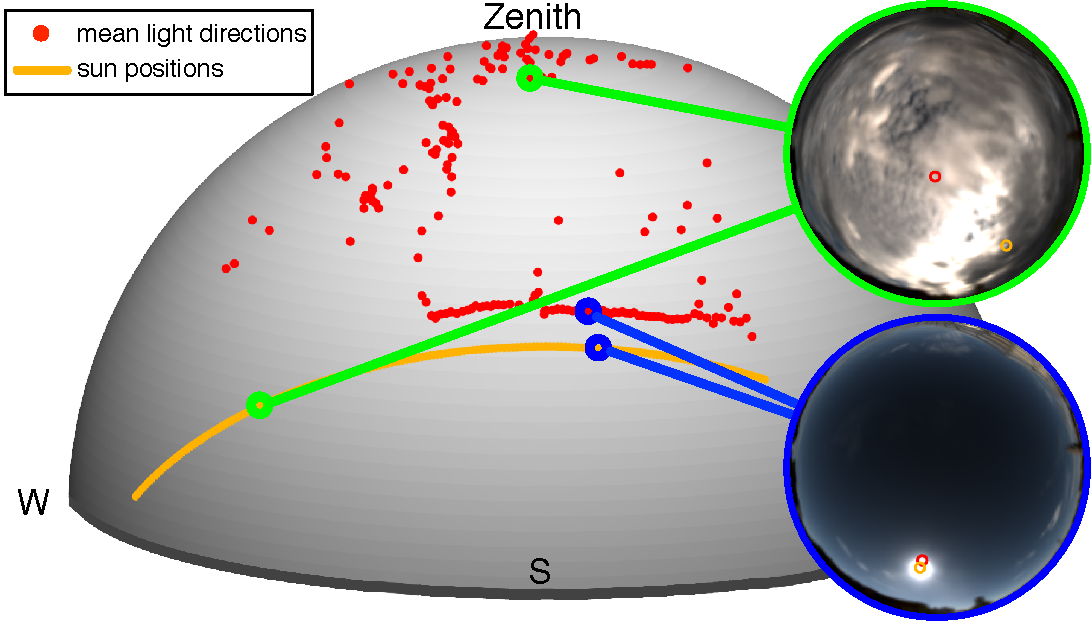
\includegraphics[width=0.5\linewidth]{./figures/mlvFig/mlvFig.pdf}
    \caption{Cloud effect on the mean light direction over one day: while the sun path (orange) yields nearly co-planar directions of illumination, the mean light directions (red dots) provide a much more varied set (data from 11/06/2013, 2nd row of fig.~\ref{fig:database}).}
    \label{fig:mlv}
\end{figure}

This key observation also demonstrates the advantages of adopting more elaborate illumination models (\eg, \cite{yu-iccp-13}). For instance, the simpler point light model was used in \cite{shen-pg-14} to study the conditioning of outdoor PS. Because the atmospheric component is not modeled, the conclusion was that single-day reconstruction breaks down in two cases of nearly coplanar sun directions: closer to the poles near the winter solstice, and worldwide near an equinox. Our results suggest that more attention should be placed on the illumination model, without focusing exclusively on the sun.

\section{Influence of sun elevation}
\label{sec:sun-elevation-results}

We also hypothesized the position of the sun to have an important effect on the ability to recover surface normals outdoors. Since our dataset is already aligned in terms of sun azimuths (see sec.~\ref{sec:hdrdb}), we now analyze the influence of sun elevation. For this purpose, we retain only the days for which the sun visibility was between 15--85\% of the time. We then compute the relation between sun elevation and expected reconstruction confidence, as illustrated in fig.~\ref{fig:sun-elevation-plot}.

Sun elevation does appear to have an influence, with higher sun elevations resulting in slightly increased uncertainty than when the sun is lower in the sky. However, the impact is less drastic than that of cloud cover from sec.~\ref{sec:cloud-cover-results}. These results can be explained, at least in part, by the smaller sun-zenith shift introduced by cloud cover when the sun is already high in the sky; therefore, smaller improvements in conditioning are obtained.

Our data-driven analysis shows that higher sun elevations---predicted as preferable by the analysis in~\cite{shen-pg-14}---are in fact not necessarily optimal when taking more elaborate illumination models into account.


% Section 3 has a note about non-coplanar sun directions  vs  non-coplanar mean light vectors (zenith, sun elevation),


\section{Analyzing full objects}

So far, our analysis has focused solely on one patch (one normal direction) at a time. But can we also say something about an entire object? Clearly, a full answer to this question would require analyzing non-local effects such as occlusions, inter-reflections, cast shadows, etc. However, we hypothesize that a simpler analysis ignoring these effects can still provide useful results. We therefore predict the performance of an outdoor PS algorithm by computing the expected value of the confidence interval, $\mathbb{E}_{\bf n}[\mathcal{C}_{\bf n}]$, over an entire object; expectation over the normal vector is computed using a prior distribution taken from a simpler convex shape (\eg, a sphere). Fig.~\ref{fig:objects} shows the expected reconstruction performance for two objects: a bottle, and the bunny. Overall, surface reconstruction performance is expected to be best when objects face south (\ie, the sun).

\begin{figure}[t]
    \centering
    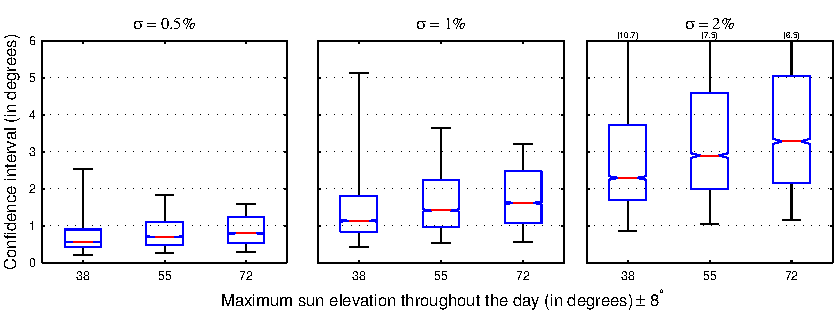
\includegraphics[width=\linewidth]{./figures/confidenceIntervals/sunElevationPlot-topHemisphere.pdf}
    \caption{Median confidence interval of normal estimates (red line) as a function of maximum sun elevation over the course of the day for various values of $\sigma$. Although the effect is not as significant as with cloud cover, we anticipate a small decrease in performance at higher sun elevations. The lower (upper) edge of each blue box indicates the 25th (75th) percentile. Statistics are computed only on normals pointing upwards to lessen ground effects.}
    \label{fig:sun-elevation-plot}
\end{figure}

% \begin{figure}[t]
%     \centering
%     \begin{sideways}\begin{minipage}{.45\linewidth}\centering \scriptsize Low elevation \vspace{5pt} \end{minipage}\end{sideways}
%     \includegraphics[width=.9\linewidth]{./figures/confidenceIntervals/elevation-low-mean_10pm.png} \\[2mm]
%     \begin{sideways}\begin{minipage}{.45\linewidth}\centering \scriptsize High elevation \vspace{5pt} \end{minipage}\end{sideways}
%     \includegraphics[width=.9\linewidth]{./figures/confidenceIntervals/elevation-high-mean_10pm.png} \\[3mm]
%     \includegraphics[width=\linewidth]{./figures/confidenceIntervals/colorbar.png}
%   \caption{Influence of sun elevation on the 95\% confidence intervals with $\sigma=1\%$. The top plot shows the mean, per-normal, confidence intervals obtained for mixed skies with low sun elevation. The bottom plot shows the same data, but for mixed skies with high sun elevation. As in fig.~\ref{fig:confidence-intervals}, the plots show the full sphere of normals from two different viewpoints: South (left), and North (right). Cardinal directions are shown for reference. The color-coding is indicated below the plots.}
%   \label{fig:sun-elevation}
% \end{figure}

\begin{figure}[t]
    \centering
    \includegraphics[width=\linewidth]{./figures/objectFig/objectFigNoise.pdf}
    \caption{Predicting object reconstruction performance for the 08/24/2013 dataset. These curves show the mean surface reconstruction variance for two objects: a bottle (blue) and the bunny (red). Irrespective of the noise level, surface reconstruction performance is expected to be best when the objects face south.}
    \label{fig:objects}
\end{figure}

\subsection{Validation on real object images}
\label{sec:validation}

The analysis performed on our dataset indicates that surface patches may be better reconstructed in certain conditions, dependent upon cloud coverage, sun elevation, and the orientation of the patch itself. At the time of this writing, a thorough validation on real outdoor images of different objects is currently under development. This section reports preliminary results on real outdoor images of an owl statuette (fig.~\ref{fig:reconstruction:example_envmaps}), which was scanned with a Creaform MetraSCAN at a resolution of 0.05mm to provide a reference of true surface orientation.

\begin{figure*}[!ht]
    \centering
    \setlength{\tabcolsep}{0pt}
    \newcommand{\customwidth}{.077\linewidth}
    \begin{tabular}{@{}rcccccccccccc@{}}
    &
    \begin{minipage}{\customwidth}\centering\scriptsize 10:30 \end{minipage} &
    \begin{minipage}{\customwidth}\centering\scriptsize 11:00 \end{minipage} &
    \begin{minipage}{\customwidth}\centering\scriptsize 11:30 \end{minipage} &
    \begin{minipage}{\customwidth}\centering\scriptsize 12:00 \end{minipage} &
    \begin{minipage}{\customwidth}\centering\scriptsize 12:30 \end{minipage} &
    \begin{minipage}{\customwidth}\centering\scriptsize 13:00 \end{minipage} &
    \begin{minipage}{\customwidth}\centering\scriptsize 13:30 \end{minipage} &
    \begin{minipage}{\customwidth}\centering\scriptsize 14:00 \end{minipage} &
    \begin{minipage}{\customwidth}\centering\scriptsize 14:30 \end{minipage} &
    \begin{minipage}{\customwidth}\centering\scriptsize 15:00 \end{minipage} &
    \begin{minipage}{\customwidth}\centering\scriptsize 15:30 \end{minipage} &
    \begin{minipage}{\customwidth}\centering\scriptsize 16:00 \end{minipage}
    \\
    \begin{sideways}\begin{minipage}{\customwidth}\centering \scriptsize illumination \\ 43\% sun vis. \\ \vspace{5pt} \end{minipage}\end{sideways} &
    \includegraphics[width=\customwidth]{./figures/reconstruction/envmaps/20141011_102928.jpg} &
    \includegraphics[width=\customwidth]{./figures/reconstruction/envmaps/20141011_110128.jpg} &
    \includegraphics[width=\customwidth]{./figures/reconstruction/envmaps/20141011_112928.jpg} &
    \includegraphics[width=\customwidth]{./figures/reconstruction/envmaps/20141011_120128.jpg} &
    \includegraphics[width=\customwidth]{./figures/reconstruction/envmaps/20141011_122929.jpg} &
    \includegraphics[width=\customwidth]{./figures/reconstruction/envmaps/20141011_130128.jpg} &
    \includegraphics[width=\customwidth]{./figures/reconstruction/envmaps/20141011_132928.jpg} &
    \includegraphics[width=\customwidth]{./figures/reconstruction/envmaps/20141011_135928.jpg} &
    \includegraphics[width=\customwidth]{./figures/reconstruction/envmaps/20141011_142928.jpg} &
    \includegraphics[width=\customwidth]{./figures/reconstruction/envmaps/20141011_145928.jpg} &
    \includegraphics[width=\customwidth]{./figures/reconstruction/envmaps/20141011_152928.jpg} &
    \includegraphics[width=\customwidth]{./figures/reconstruction/envmaps/20141011_155928.jpg}
    \\
    \begin{sideways}\begin{minipage}{.106\linewidth}\centering \scriptsize object capture \\ \vspace{1em} \vspace{5pt} \end{minipage}\end{sideways} &
    \includegraphics[width=\customwidth]{./figures/reconstruction/object/103307.jpg} &
    \includegraphics[width=\customwidth]{./figures/reconstruction/object/110346.jpg} &
    \includegraphics[width=\customwidth]{./figures/reconstruction/object/113346.jpg} &
    \includegraphics[width=\customwidth]{./figures/reconstruction/object/120346.jpg} &
    \includegraphics[width=\customwidth]{./figures/reconstruction/object/123346.jpg} &
    \includegraphics[width=\customwidth]{./figures/reconstruction/object/130215.jpg} &
    \includegraphics[width=\customwidth]{./figures/reconstruction/object/133215.jpg} &
    \includegraphics[width=\customwidth]{./figures/reconstruction/object/135615.jpg} &
    \includegraphics[width=\customwidth]{./figures/reconstruction/object/143215.jpg} &
    \includegraphics[width=\customwidth]{./figures/reconstruction/object/150215.jpg} &
    \includegraphics[width=\customwidth]{./figures/reconstruction/object/153215.jpg} &
    \includegraphics[width=\customwidth]{./figures/reconstruction/object/160215.jpg}

    \end{tabular}
    \caption{Real outdoor HDR images of owl statuette and corresponding HDR environment maps (top row) providing synchronized, high-fidelity estimates of illumination conditions. All images were acquired on 10/11/2014 and tone-mapped for display only (with $\gamma = 1.6$). The sun visibility was 43\% on this day. }
    \label{fig:reconstruction:example_envmaps}
    \vspace{-1em}
\end{figure*}

We oriented this owl statuette towards south and took 66 HDR captures using a Canon EOS Rebel SL1 between 10h30 and 16h30, local time, in Quebec City. These captures were synchronized with the HDR environment maps described in sec.~\ref{sec:hdrdb}, providing high fidelity estimates of the illumination conditions for each image, as shown in fig.~\ref{fig:reconstruction:example_envmaps}. The laser scan was then manually aligned to these images.

A simple outdoor PS algorithm was run on evenly distributed patches on the owl images. For each patch, the surface normal is obtained as to minimize the rendering error given by the model in~\eqref{eqn:matrix-form}, in a least-squares sense. Since this estimation problem is nonlinear on the normal ${\bf n}$, a solution is computed via exhaustive search on a set of 271 candidate orientations for the light hemisphere $\Omega_{\bf n}$. Given $\Omega_{\bf n}$, a candidate solution ${\bf x}$ is obtained via linear least squares. For the best solution, an estimation error, in degrees, is computed using the reference normal from the laser scan. The uncertainty measure (confidence interval $\mathcal{C}_{\bf n}$) derived in sec.~\ref{subsec:measure_uncertainty} is also computed for each patch.

Results from this quantitative evaluation are given in fig.~\ref{fig:reconstruction:results}. As shown on the left, normals pointing upwards are generally recovered more accurately than normals pointing downwards. This is in concordance with the predicted confidence intervals shown on the right in fig.~\ref{fig:reconstruction:results}. The behavior of the reconstruction error is, in general, well predicted by the confidence intervals.
% Note however that the ground truth normals were aligned with the images manually, therefore slight misalignments could explain discrepancies.


\begin{figure}[t]
    \centering
    \begin{minipage}{0.5\linewidth}
    \newcommand{\customwidthres}{0.45\linewidth}
    \begin{tabular}{cc}
        \scriptsize Angular differences to ground truth & \scriptsize Predicted 95\% confidence intervals \\
        \includegraphics[width=\customwidthres]{./figures/reconstruction/owl_delta_gt.png} &
        \includegraphics[width=\customwidthres]{./figures/reconstruction/owl_confint.png}
        \begin{picture}(0,0)
            \put(-155,-2){\includegraphics[height=1.5cm]{./figures/reconstruction/owl_sphere_dgt.png}}
            \put(-35,-2){\includegraphics[height=1.5cm]{./figures/reconstruction/owl_sphere_ci.png}}
        \end{picture}
    \end{tabular}
    \includegraphics[width=1.01\linewidth]{./figures/reconstruction/colorbar.png}
    \end{minipage}
    \caption{Quantitative validation on images of a real object. Evenly distributed patches of the owl images were used to perform a simple calibrated outdoor PS algorithm. Error estimates of the surface normals are reported on the left using the reference surface orientation in the laser scan. The predicted 95\% confidence intervals $\mathcal{C}_\mathbf{n}$ from \eqref{eqn:confidence-degrees} are shown on the right. A few large estimation errors on the left image may be caused by imperfect alignment between the scanned model and the images. Insets in the lower right corner show the recovered normals mapped to the south hemisphere. Normals in dark blue means no data available.}
    \label{fig:reconstruction:results}
\end{figure}


% !TEX root = main.tex


%\subsection{Outdoor PS conditioning}
%\label{sec:sensitivity-analysis}

%In the following, we consider a small planar surface patch with normal vector ${\bf n}$ and Lambertian reflectance with albedo~$\rho$. As discussed in~\cite{holdgeoffroy-iccp-15,hung-wacv-15}, the lighting contribution of an environment map to a Lambertian surface patch can be formulated as in an equivalent problem with a single point light source $\bar{\mathbf{l}} \in \mathbb{R}^3$. This vector is the mean of the light vectors computed over the hemisphere of incoming light directions defined by ${\bf n}$. This virtual point light source $\bar{\mathbf{l}}$ is henceforth referred to as the {\em mean light vector} (MLV). It is important to note that, as opposed to the traditional PS scenario where point light sources are fixed and thus independent of ${\bf n}$, here the {\em per-pixel} MLV is a function of $\mathbf{n}$. Thus, patches with different orientations define different sets of MLVs (as discussed later and shown in fig.~\ref{fig:realShiftNormal}).

%Given multiple images of the same patch, taken at different times, we collect all photometric constraints for that patch and obtain the PS equation in matrix form:
%
%\begin{equation}
%\mathbf{b} =
%\begin{bmatrix}
% b_1 \\ b_2 \\ \vdots \\ b_T
%\end{bmatrix}
%= 
%\begin{bmatrix}
% {\bf \bar l}_1^T \\ {\bf \bar l}_2^T \\ \vdots \\ {\bf \bar l}_T^T
%\end{bmatrix}
%{\bf x} = \mathbf{L} \mathbf{x} \,,
%\label{eqn:matrix-form}
%\end{equation}
%
%where $b_i \in \mathbb{R}$ are the observed pixel intensities, and ${\bf x} \in \mathbb{R}^3$ is the surface normal ${\bf n}$ scaled by $\rho$.

%Let $\hat{{\bf x}}=({\bf L}^T{\bf L})^{-1}{\bf L}^T{\bf b}$ denote the least-squares solution of~\eqref{eqn:matrix-form}. A 95\% confidence interval for normal ${\bf x}$ is given by 
%
%\begin{equation}
%\hat{\mathbf{x}} \pm \bolddelta \,, \quad \text{with } \delta_k = 1.96 \frac{\sigma}{\rho}\lambda_k \,,
%\label{eqn:confidence-xyz}
%\end{equation}
%
%where $\sigma$ is the camera noise level and $\lambda_k$ is the square root of the $k$-th element on the diagonal of $({\bf L}^T{\bf L})^{-1}$~\cite{hastie-book-09}. 

% A more intuitive measure of uncertainty in the estimate $\hat{{\bf n}}$ is obtained by considering angular distances $\theta$ in degrees, 
% % 
% \begin{equation}
% \theta^\pm = \cos^{-1}({\bf \hat n}^T{\bf \hat n}^\pm)\,, 
% \quad \text{where }
% {\bf \hat n}^\pm = \frac{{\bf \hat n} \pm \bolddelta}{\lVert{\bf \hat n} \pm \bolddelta \rVert}.
% \label{eqn:angular-dist}
% \end{equation}
% %
% Our measure of uncertainty, or stability, in the estimation of ${\bf \hat n}$ is then defined as the confidence interval \mbox{$\mathcal{C}_{\bf n} = [ 0, \max(\theta^\pm) ]$} in degrees.

% In the analysis below, we often take the estimate ${\bf \hat n}$ to be the ground truth normal ${\bf n}$ of a simulated (synthetic) surface patch; this corresponds to the result of an ideal algorithm. We then evaluate the confidence interval for this normal using a set of real, outdoor environment maps with associated stability parameters $\lambda_k$ as in~\eqref{eqn:confidence-xyz}. The result is a measure of the uncertainty in the reconstruction that an actual outdoor PS algorithm would provide on that particular set of illumination conditions, and surface orientation. As in~\cite{holdgeoffroy-iccp-15}, our simulations below consider synthetic surface patches with albedo $\rho = 1$ and a small, non-negligible noise level $\sigma$ at $1\%$ of the maximum pixel value.


\section{$x$-hour outdoor PS}
%\subsection{Time interval analysis}
\label{sec:ch1_analysis}

we push the analysis of sec.~\ref{iccp15} to the limit to see what is the minimum capture interval required by PS to work. We do so by tying what is happening in the sky to reconstruction performance. The analysis is done, as before, only images that were captured during a continuous 6 hour time interval on each of these days, from 10:30 until 16:30.\footnote{Companion video showing data samples available at \url{http://vision.gel.ulaval.ca/~jflalonde/projects/xHourPS/}.}

From the 95\% confidence interval \eqref{eqn:confidence-xyz}, we can deduce that the only light-dependent stability factor in the confidence interval $\bolddelta$ is $\lambda_k$; the other two factors are related to the camera ($\sigma$), and surface reflectance~($\rho$). In this paper, we analyze the maximum uncertainty \mbox{$\lambda_\text{max} = \max_k(\lambda_k)$}, as a conservative performance measure that is independent of albedo and sensor noise; $\lambda_\text{max}$ is a {\em maximum noise gain} factor, \ie, the intensity of noise amplification in the solution. Here, we are interested in 1) investigating how the noise gain $\lambda_\text{max}$ is influenced by the duration of outdoor data capture, and in 2) identifying specific changes, or {\em events}, in outdoor lighting that are associated with more stable PS solutions (smaller $\lambda_\text{max}$).

To make our analysis tractable, we do not model cast shadows and inter-reflections. In addition, we assume that the sky hemisphere (around zenith) provides the dominant part of incoming light. Unless stated otherwise, our simulations consider a day near an equinox, which corresponds to the worst case scenario with coplanar sun directions~\cite{shen-pg-14}.

\todo{define MLV}

This section provides the first answers to the questions raised above by looking at collections of mean light vectors (MLVs) from both simulated and real sky data. The main goal is to analyze the behavior of the illumination factors $\lambda_k$ (and associated confidence interval) of normal estimation. More specifically, we investigate numerical stability (MLV coplanarity) as a function of the apparent sun motion and cloud coverage within capture intervals of different durations, containing different atmospheric events. We also compare the resulting performance measures of $x$-hour outdoor PS to those of full-day outdoor PS.

% Here our goal is to answer the questions: \emph{what} are the important changes, or {\em events}, in outdoor lighting that affect $\lambda_k$? What is the minimum duration of data capture, containing one or more of such events, that can lead to performance similar to that of full-day PS?

% -----------------------------------------------------------------------------
\begin{figure}[t]
\centering
\includegraphics[width=.33\columnwidth]{diagram_MLVshift3}
\caption{Impact of cloud coverage on the numerical conditioning of outdoor PS: clear (a) and overcast (b) days present MLVs with stronger coplanarity; in partly cloudy days (c) the sun is often obscured by clouds, which may lead to out-of-plane shifts of MLVs.}
\label{fig:MLVshift}
\end{figure}
% -----------------------------------------------------------------------------
% -----------------------------------------------------------------------------
\begin{figure*}[t]
\centering
\includegraphics[width=.32\textwidth]{v123gainSurf} \ \ \ %\\[3mm]
\includegraphics[width=.32\textwidth]{v123gain1Arc} \ \ \ %\\[3mm]
\includegraphics[width=.32\textwidth]{v123gain2Shift}
\caption{Simulated noise gain $\lambda_{\max}(\theta_a,\theta_e)$ as a function of solar arc $\theta_a$ and MLV shift (elevation) angle $\theta_e$. See discussion in the text.}
\label{fig:v123gain}
\end{figure*}
% -----------------------------------------------------------------------------

\section{Cloud coverage and MLV shifting}
\label{subsec:mlv-clouds}

As shown in~\cite{holdgeoffroy-iccp-15}, with data captured under clear skies, the MLVs of the model above will point nearly towards the sun, from which arrives most of the incoming light. Thus, near an equinox (worldwide), the resulting set of MLVs are nearly coplanar~\cite{shen-pg-14}, resulting in poor performance, fig.~\ref{fig:MLVshift}(a). For a day with an overcast sky, performance is also poor because the set of MLVs are nearly colinear and shifted towards the patch normal ${\bf n}$, fig.~\ref{fig:MLVshift}(b). Finally, in partly cloudy days (mixed skies), the sun is often obscured by clouds and such occlusion shifts some MLVs away from the solar plane, improving numerical stability, fig.~\ref{fig:MLVshift}(c). 

% NOT SURE ABOUT THIS ANYMORE:
% This improvement in conditioning is more significant with lower sun elevations, as the MLVs are shifted towards zenith.


\section{Solar arcs and MLV elevation}
\label{subsec:solararcs-mlvelevation}

%If we assume equinox, then the sun actually moves on a plane worldwide (i.e. independent of latitude) and is also visible 12 hours worldwide (although terrain and atmosphere play a small role and change that). Thus, this simulation requires the equinox assumption. What does vary with latitude (at equinox) is: (1) the inclination of the solar plane, and (2) the frequency of cloud coverage (if the sun is lower in the sky most of the day). Anything else?

Here, we seek to provide a sense of the minimal length of solar arc and amount of out-of-plane MLV shift required in single-day outdoor PS.

Assuming a day near an equinox, the apparent sun trajectory worldwide describes an arc $\theta_a$ within the solar plane of about $15^\circ$ per hour. We now use this observation to evaluate the numerical stability of outdoor PS for data capture intervals (solar arcs) of different lengths. Considering a partly cloudy sky, we also investigate the interaction of solar arc and cloud coverage; we quantify performance as a function of both acquisition time (solar arc $\theta_a$) and amount of out-of-plane MLV shift (elevation angle $\theta_e$) introduced by clouds.

A simple and effective way to investigate conditioning with different capture scenarios is to consider a simulation with the minimum number of three MLVs, as required for outdoor PS using~\eqref{eqn:matrix-form}. We simulate solar arcs $\theta_a$ of different lengths by defining two MLVs on a reference solar plane, with the third MLV presenting varying elevation $\theta_e$ away from this plane, as illustrated in fig.~\ref{fig:MLVshift}(c). The actual orientation of the solar plane varies with the latitude of the observer; thus, we represent MLV shift relative to this plane.

The numerical conditioning of outdoor PS, as observed with different configurations for these three MLVs, is then scored using the noise gain~$\lambda_{\max}$ (sec.~\ref{sec:sensitivity-analysis}). This measure is independent of albedo and sensor noise; it is also related to the condition number of the illumination matrix ${\bf L}$ in~\eqref{eqn:matrix-form}.

% Lower bound as MLV intensity is reduced by cloud coverage; thus MLV elevation need to be higher, actually.

% define full day as 6-hour outdoor PS (shadowing concerns)?

We compute~$\lambda_{\max}(\theta_a,\theta_e)$ for solar arcs $\theta_a$ of up to 6 hours ($90^\circ$) and MLV elevations $\theta_e$ up to $90^\circ$. For simplicity, we consider triplets of unit-length MLVs---thus, conditioning depends on the magnitude $\sin(\theta_e)$ of the out-of-plane component of the third MLV. Clearly, the optimal noise gain~$\lambda_{\max} = 1$ is obtained when the MLVs are mutually orthogonal ($\theta_a = \theta_e = 90^\circ$).

Fig.~\ref{fig:v123gain}(a) shows that the noise gain $\lambda_{\max}$ drops quickly to under 6 for capture intervals at just above 1 hour and for MLV shifts $\theta_e > 15^0$. This result suggests that even the performance of 1-hour PS can be acceptable with small levels of sensor noise $\sigma$ and high surface reflectance $\rho$. To ease visualization, figs.~\ref{fig:v123gain}(b,c) show cross sections of the $\lambda_{\max}(\theta_a,\theta_e)$ gain surface for a constant shift or solar arc.

A second important prediction from fig.~\ref{fig:v123gain}, considering (more realistic) small to moderate amounts of MLV shifts $\theta_e \leq 40^\circ$, is that conditioning will improve very little for data capture intervals above 3 hours ($45^\circ$ solar arcs). Reducing data capture from 3 to 2 hours would lead to an additional increase in uncertainty ($\lambda_{\max}$) of less than $30\%$ (from about 2.8 to nearly 3.6). Still, 2-hour outdoor PS with noise gains under $4\times$ may be possible if an MLV shift of $\theta_e > 20^\circ$ is introduced by atmospheric events during capture. Uncertainty in the results of 1-hour outdoor PS would be about 5 to 7 times that of full-day (6-hour) outdoor PS.


\section{MLV shifts in real sky probes}

% how much MLV shift is expected?
% but how much uncertainty can we expect? look into real sky probes...
% Here we evaluate the actual noise gain from real data... 
% pick days near equinox to isolate shifting due to clouds only (really needed?)
% TODO: What happens with natural sun elevation in summer (non-equinox), high-latitude? sun declination angle of $23.5^\circ$. The other two vectors are always on plane!

% what we do: look at gain to infer elevation, we fit solar arc for clear sky, look at orthogonal component of MLVs
% for each normal visible to the camera, we plot the best gain computed from the solar plane and a third MLV
% does enough shift really happen? how much shift and for which normals?
% average/pattern over multiple days?

While the analysis above suggests that outdoor PS may be possible with a capture interval of only about 1 to 3 hours, it does not answer whether it is possible to observe an adequate amount of MLV shift (elevation away from solar plane) within a single partly cloudy day. In the following, we analyze the shifting (coplanarity) of real MLVs obtained from a database of real environment maps (sky probes)~\cite{holdgeoffroy-iccp-15}.

% MLV shifting depends on which portion of the sky the normal (patch) sees.
% shifting varies with normal (examples, more in suppl video)
% dimming in overcast (early morning/afternoon) affects conditioning too (explain)

First, it is important to note that surface patches of different orientations (normals) are exposed to different hemispheres of illumination, with light arriving from above (sky) and below (ground). This fact is illustrated in fig.~\ref{fig:realShiftNormal} for three different normal vectors (rows) and two different days (columns). Each globe represents the coordinate system for the environment maps captured in a day. For each combination normal-day, the time-trajectory of computed MLV directions (dots) and intensities (colors) are shown on the globe. Brighter MLVs lie closely to the solar arc, while darker MLVs may shift away from it. 

To more closely match the scenario considered above, we scale these real MLVs so that the brightest one over all days (\ie, for the most clear sky) has unit-length. From fig.~\ref{fig:realShiftNormal}, also note that some MLVs are shifted very far from the solar arc but, as indicated by the darker colors, their intensity is dimmed considerably by cloud coverage; little improvement in conditioning is obtained from these MLVs.

Most important, fig.~\ref{fig:realShiftNormal} shows that the amount of out-of-plane MLV shift (elevation) relative to the solar arc also depends on the orientation ${\bf n}$ of the surface patch. This suggest that outdoor PS reconstruction may present different amounts of uncertainty (conditioning) depending on the normal of each patch. Indeed, the noise gain ($\lambda_{\max}$) values in fig.~\ref{fig:realShiftAll} show that patches with nearly horizontal normals (orthogonal to the zenith direction) are associated with sets of MLVs that are closer to being coplanar throughout the day. As expected, patches oriented towards the bottom also present worse conditioning since they receive less light.

% Normals nearly horizontal are worse, why? Interesting!
% Uncertainty is higher, more errors, suggest direction for future investigation

Although these MLVs were computed from environment maps captured in the Northern hemisphere (Pittsburgh, USA, and Quebec City, Canada~\cite{holdgeoffroy-iccp-15}), similar conclusions can be drawn for the Southern hemisphere. Finally, note that this section has considered MLV shifts in whole-day datasets. Next, we look at subsets of MLVs from time intervals of varying lengths and analyze some of the atmospheric events associated with improved conditioning.

% Next, we look into real datasets of partly cloudy skies and measure the actual amount of MLV shifting for hypothetical capture sessions of varying duration, from 1 to 6 hours. 


% -----------------------------------------------------------------------------
\begin{figure}[t]
\centering
\hspace{3.1cm} \includegraphics[width=2.6cm]{sphere_key_bold} \\[-1mm]
\includegraphics[height=1.43in]{sphereShift20131106_n1} \ \ %\\[3mm]
\includegraphics[height=1.43in]{sphereShift20141011_n1} \\[3mm]
\includegraphics[height=1.43in]{sphereShift20131106_n2} \ \ %\\[3mm]
\includegraphics[height=1.43in]{sphereShift20141011_n2} \\[3mm]
\includegraphics[height=1.43in]{sphereShift20131106_n3} \ \ %\\[3mm]
\includegraphics[height=1.43in]{sphereShift20141011_n3} \\[2mm]
{\footnotesize {\verb| |} \hspace{0.5cm} (a) Mixed clouds (06-NOV-13) \hspace{0.25cm} (b) Mixed clouds (11-OCT-14) }\\
\vspace{-2mm}
\caption{Globes representing the coordinate system of sky probes. Each normal (blue arrow) defines a shaded hemisphere in the environmental map that does not contribute light to the computed MLVs (dots). All MLVs in two particular partly cloudy days (columns) were computed from real environment maps~\cite{holdgeoffroy-iccp-15} for 3 example normal vectors (rows). Relative MLV intensities are shown in the color bar on the left. See also video in~\cite{webpageXhourPS}.}
\label{fig:realShiftNormal}
\vspace{-3mm}
\end{figure}
% -----------------------------------------------------------------------------
% -----------------------------------------------------------------------------
\begin{figure}[!ht]
\centering
\includegraphics[height=1.46in]{sphereGain20131106} \ \ \ %\\[3mm]
\includegraphics[height=1.46in]{sphereGain20141011} \\[1mm]
{\footnotesize {\verb| |} \hspace{.6cm} (a) 06-NOV-13 \hspace{1cm} (b) 11-OCT-14 }\\[3mm]
\vspace{-2mm}
\caption{Noise gain for each normal direction ${\bf n}$ visible to the camera; the colors indicate the shifting (coplanarity) of the associated MLVs. The camera is assumed to lie to the South of this hypothetical target object. For both days, normals that are nearly horizontal are associated with more coplanar MLVs (smaller shifts, higher gains). These normals define a {\em zero-crossing region} between positive and negative out-of-plane shifts (mid row in fig.~\ref{fig:realShiftNormal}), where occlusion of the sun results in shifts that are predominantly {\em along} the solar arc. See also video available in~\cite{webpageXhourPS}.}
\label{fig:realShiftAll}
\vspace{-3mm}
\end{figure}
% -----------------------------------------------------------------------------


\section{Evolution of noise gain over time}

In this section, we show how the conditioning of outdoor PS evolves over time. Analyzing the patterns in its evolution will allow us to isolate important ``events''---points at which uncertainty suddenly drops---and investigate whether such events occur in close succession.

The main results are given in fig.~\ref{fig:events}, which plots the gain factor $\lambda_{\max}$ for all possible time intervals in four different days. Since $\lambda_{\max}$ varies with ${\bf n}$, we plot the median gain over 321 normal vectors visible to the camera (by subdividing an icosahedron three times) for each time interval.

The first row of fig.~\ref{fig:events}(a,b) illustrates the case of two days identified in sec.~\ref{subsec:mlv-clouds} as yielding poor outdoor PS reconstructions. As seen in the plots, low noise gains are never reached, irrespective of the start time and duration of the capture interval. We note that the (nearly) overcast sky of fig.~\ref{fig:events}(b) exhibits better behavior than the completely clear sky of fig.~\ref{fig:events}(a). This is because that day is not completely overcast, and the sun sometimes becomes visible (see the sun log-intensity plot). MLVs are thus shifted away from their main axes, while improving conditioning only slightly.

More interesting scenarios arise on days exhibiting a better mix of sun and moving clouds, such as the two examples in fig.~\ref{fig:events}(c,d). The two black vertical lines in fig.~\ref{fig:events}(c) identify capture intervals starting at two different times. Following the line labeled ``start time 1'' (beginning at 11:00), we notice that uncertainty remains high for approximately two hours, then suddenly drops at around 13:00. This time instant is followed by sudden changes in sun intensity (due to passing clouds) that are sufficient to shift the MLV away from the sun plane. Subsequently, uncertainty continues to decrease, albeit at a much slower pace, over the rest of the day. The second time interval (identified as ``start time 2'') starts at 14:00, so it does not benefit from that period of sun intensity changes. The maximum gain at the end of the interval is therefore higher. 

Of course, this could be due to a simple fact: the first interval is longer than the second one. However, fig.~\ref{fig:events}(d) shows that longer intervals do not always result in lower uncertainty. This time, two 2-hour intervals are considered. The time interval labeled as ``start time 1'' stops right before the 14:00 mark, and only sees clear skies; as expected, the uncertainty is very high. ``Start time 2'', beginning at 13:30, can fully exploit the MLV shifts caused by moving clouds to dramatically decrease PS uncertainty, even while the interval length is kept constant.
  
\begin{figure*}[!th]
\centering
\footnotesize
\setlength{\tabcolsep}{0pt}
\begin{tabular}{cc}
\includegraphics[height=4.7cm]{./figures/events/events-20141003-colorbar.pdf} & 
\includegraphics[height=4.7cm]{./figures/events/events-20131119-colorbar.pdf} \\
(a) Clear day (03-OCT-14) & (b) Nearly overcast day (19-NOV-13) \\%*[.5em]
% \multicolumn{2}{c}{\includegraphics[width=.3\linewidth]{./figures/events/colorbar-horizontal-withlegend.pdf}} \\%*[.5em]
\includegraphics[height=4.7cm]{./figures/events/events-20130824-colorbar.pdf} & 
\includegraphics[height=4.7cm]{./figures/events/events-20131106-colorbar.pdf} \\
(c) Clear sky and mixed clouds (24-AUG-13) & (d) Mixed clouds (06-NOV-13)
\end{tabular}
\vspace{.25em}
\caption{Fine-grained analysis of the expected uncertainty of outdoor PS as a function of time over four selected days in the dataset. Colored plots show the maximum gain $\lambda_\text{max}$ as a function of start time (diagonal along the plot), and duration of the interval. The black lines identify particular time intervals discussed in the text. The blue curve to the left of each colored plot represents the log sun intensity over the course of that day. Photographs of the sky for each day are also shown on the left.}
\label{fig:events}
\end{figure*}

\section{Overall performance of $x$-hour PS}  

We noted in fig.~\ref{fig:events}(d) that sufficient conditions for low uncertainty could be met in as little as 2 hours. In this section, we evaluate how often one can achieve low uncertainty in short time intervals. This is done by assessing the distribution of noise gains from short time intervals, and aggregating results over multiple days.

To compute these statistics, we first consider a single normal and a single day. For a particular time interval \mbox{$\tau = \{t_\text{start}, t_\text{end}\}$}, we compute the ratio $r_\lambda(\tau)$ of its noise gain divided by the best (minimum) gain of all possible intervals in this day (including the full-day interval). Fig.~\ref{fig:ratios}(a,b) shows distributions of relative gains $r_\lambda$ for the two days in fig.~\ref{fig:events}(c,d). Fig.~\ref{fig:ratios}(a) shows that, for intervals of 4 hours, 75\% of the normals have uncertainty below twice the minimum gain for that day. In the case of fig.~\ref{fig:ratios}(b), that interval drops to 3 hours. 

The ratios $r_\lambda$ were then computed for all normals, over all days in the database. The compound statistics are shown in fig.~\ref{fig:ratios}(c). They empirically illustrate that there were many opportunities for stable normal reconstruction with short capture intervals. For example, more than 50\% of the time intervals of 3 hours resulted in reconstructions that had at most twice the uncertainty of the optimal interval. These results suggest that opportunities for shorter capture sessions seem to occur quite frequently in practice.

\begin{figure*}
    \footnotesize
    \centering
    \begin{tabular}{ccc}
    \setlength{\tabcolsep}{0pt}
    \includegraphics[width=.30\linewidth]{./figures/relativePerf/20130824-maxGain-global-relativePerf.pdf} & 
    \includegraphics[width=.30\linewidth,height=.202\linewidth]{./figures/relativePerf/20131106-maxGain-global-relativePerf.pdf} & 
    \includegraphics[width=.30\linewidth]{./figures/relativePerf/all-maxGain-relativePerf.pdf} \\
    (a) 24-AUG-13 & (b) 06-NOV-13 & (c) Entire dataset
    \end{tabular}
    \vspace{.15em}
    \caption[]{Distribution of noise gain ratio $r_\lambda(\tau)$ as a function of time interval duration: (a,b) two days in fig.~\ref{fig:events}; (c) across all the dataset. The~distributions of computed ratios are displayed vertically as ``box-percentile plots''~\cite{esty-jss-03}; the red horizontal bars indicate the median, while the bottom (top) blue bars are the 25th (75th) percentiles. }
    % THIS IS CONFUSING, DOESN'T HELP MUCH:
    %Note that durations include all intervals within $\pm 30\text{m}$ of the value indicated. For example, a duration of 4h includes all time intervals in the range $[3\text{h}30, 4\text{h}30]$.
    \label{fig:ratios}
\end{figure*}

%\begin{figure}
%\centering 
%\footnotesize
%\setlength{\tabcolsep}{0pt}
%\begin{tabular}{cc}
%\includegraphics[width=.49\linewidth]{./figures/relativePerf/20130824-cn-local-relativePerf.pdf} & 
%\includegraphics[width=.49\linewidth]{./figures/relativePerf/20131106-cn-local-relativePerf.pdf} \\
%(a) 24-AUG-13 & (b) 06-NOV-13
%\end{tabular} 
%\includegraphics[width=.49\linewidth]{./figures/relativePerf/all-cn-relativePerf.pdf} \\
%(c) Entire dataset
%\vspace{.25em}
%\caption[]{Distribution of condition number ratio $r_t$ as a function of time interval duration, shown for (a,b) the same days as fig.~\ref{fig:events}, and (c) across the entire dataset. To display this ratio, we use ``box-percentile plots''~\cite{esty-jss-03}, which illustrate the distribution of ratios vertically. The red horizontal bars indicate the median, while the bottom (top) blue bars are the 25th (75th) percentiles. The outliers, illustrated by the long vertical tails above the 75th percentile, are due to normals pointing downwards, for which the expected uncertainty always remains high. Note that durations include all intervals withing $\pm 30\text{m}$ of the value indicated. For example, a duration of 4h includes all time intervals in the range $[3\text{h}30, 4\text{h}30]$. }
%\label{fig:ratios}
%\end{figure}


\begin{figure*}[t]
    \centering
    \footnotesize
    \begin{tabular}{cc}
        \includegraphics[height=4.7cm]{./figures/owl/owl-12h.pdf} & 
        \includegraphics[height=4.7cm]{./figures/owl/owl-13h30.pdf} \\
        (a) Intervals starting at 12:00 on 06-NOV-13 & (b) Intervals starting at 13:30 on 06-NOV-13
    \end{tabular}
    \vspace{1mm}
    \caption{Normal recovery error as a function of time interval and start time: (a) 12h00 and (b) 13h30 on 06-NOV-13. Experiments are performed on a synthetic object rendered with real sky probes and additive Gaussian noise $\sigma=1\%$. The top row shows per-pixel angular error, color-coded as in the scale on the right. The bottom row shows box-percentile error plots (see fig.~\ref{fig:ratios}). As suggested in fig.~\ref{fig:events}(d), the performances of \{3,4,5,6\}-hour outdoor PS are very similar (a). Even 1-hour outdoor PS can be competitive if started at the right time (b).}
    \label{fig:owl-results}
    \vspace{-3mm}
\end{figure*}

\begin{figure}[!t]
    \centering
    \includegraphics[width=.52\linewidth]{./figures/realData/realData-setup.pdf} \\[1mm]
    \caption{Real data capture setup. HDR photographs of the sky and of the object (owl statuette) are simultaneously captured by two cameras installed on the roof of a tall building.}
    \label{fig:real-data-setup}
    \vspace{-2mm}
\end{figure}

\begin{figure*}[t]
    \centering
    \includegraphics[width=0.92\linewidth]{./figures/realData/realData4.pdf}
    \caption{Validation on real data, captured on 11-OCT-14 (partly cloudy). Four distinct time intervals are analyzed and, for each one, the following information is displayed, from left to right: ($i$) log sun intensity; ($ii$) noise gain $\lambda_\text{max}$ as a function of start time and duration of the interval, as in fig.~\ref{fig:events}; ($iii$) example input images; ($iv$) normals recovered by calibrated outdoor PS; ($v$) normal estimation error at each pixel; and ($vi$) the error distribution, in degrees. For reference, ground truth normals are given on the rightmost plots.}
    \label{fig:real-results}
    \vspace{-2mm}
\end{figure*}

\subsection{Experimental validation}

We validate the analyses in sec.~\ref{sec:sensitivity-analysis} and \ref{sec:ch1_analysis} via calibrated outdoor PS on synthetic and real object images with known ground truth normals. These normals are used as an optimal initialization for computing ground-truth MLVs, thus avoiding convergence issues of nonlinear optimization and allowing us to focus on assessing errors due to illumination effects in the real sky probes. We then perform calibrated outdoor PS on these images using the algorithm in \cite{yu-iccp-13}, with the following two differences: (\emph{i}) we use all possible pairs of images to compute ratios, instead of selecting a single denominator image; and (\emph{ii}) we apply anisotropic regularization~\cite{hernandez-pami-11} to mitigate the impact of badly-conditioned pixels on the surface reconstruction.

%
\vspace{-3mm}
\paragraph{Synthetic data}%
%
We first consider synthetic images of an owl model rendered with real sky probes. The rendered images were perturbed with additive Gaussian noise at 1\% the median pixel intensity. For each image, one real-world environment map from the database was used as the sole light source. Cast shadows were not simulated to isolate the analysis to the photometric cue alone (see~\cite{webpageXhourPS} for more realistic results with a physically-based rendering engine). 

% \begin{figure}
% \centering
% \newlength{\mylength}
% \setlength{\mylength}{.19\linewidth}
% \todo{Replace with renderings with luxrender... }
% \caption{Example renderings of the owl model used in the validation experiments for 06-NOV-13 (see figs~\ref{fig:events}, \ref{fig:owl-results}). Images are tone-mapped for display ($\gamma=1.8$).}
% \label{fig:owl-synthetic-data}
% \vspace{.5em} 
% \end{figure}

We ran calibrated outdoor PS on all time intervals starting at 12:00 or 13:30 for the day 06-NOV-13 (see fig.~\ref{fig:events}(d)), in increments of one hour. The main results of this experiment are shown in fig.~\ref{fig:owl-results}. Fig.~\ref{fig:owl-results}(a) follows ``start time 1'' in fig.~\ref{fig:events}(d); the reconstruction error improves significantly until an interval of 3 hours is reached, at which point the error improves only slightly through the rest of the day. Thus, the additional data provides little new information. In fig.~\ref{fig:owl-results}(b), we now follow the path of ``start time 2'' in fig.~\ref{fig:events}(d); in this case, the error is already quite low after just one hour.
%
\vspace{-3mm}
\paragraph{Real data}%
%
Another similar experiment considered real photos of a real owl statuette. To capture this data, we set up two cameras on the roof of a tall building as shown in fig.~\ref{fig:real-data-setup}. The first camera, dubbed ``sky camera'', captures omnidirectional photos of the sky using the approach proposed by Stumpfel \etal~\cite{stumpfel-afrigraph-04}. The second, ``object'' camera is equipped with a telephoto zoom lens and captures photos of the statuette. Both cameras capture exposure-bracketed HDR photos simultaneously, once every two minutes\footnote{Data and source code are available on our project webpage~\cite{webpageXhourPS}.}. Ground truth surface normals were obtained by aligning a 3D model of the object (obtained with a 3D scanner) to the image using POSIT~\cite{dementhon-ijcv-95}. 

The validation results with real data are shown in fig.~\ref{fig:real-results}. As predicted by the noise gain values of fig.~\ref{fig:real-results}~(left), similar reconstruction performance is obtained from three different time intervals shown in the top three rows of fig.~\ref{fig:real-results}~(right). Once again, the performances of 1-hour (15:30--16:30) and 3.5-hour (13:00--16:30) outdoor PS are indeed quite close to that of ``full-day'' outdoor PS (10:30--16:30). However, not all one-hour intervals are equally good, as shown for the interval 12:00--13:00 at the bottom of fig.~\ref{fig:real-results}.


%\section{Discussion}
\section{Discussion and future work}
\label{sec:3dv-discussion}
\label{sec:iccp-discussion}

This chapter has presented the first data-driven analysis of the expected behavior of PS under outdoor illumination\cite{Hold-Geoffroy-ICCP15,Hold-Geoffroy-3DV15}. In this scenario, we have no control over the illumination conditions themselves, so existing methods to determine an optimal illumination setup~\cite{drbohlav-iccv-05,klaudiny-prl-14} cannot be applied. Our goal is, therefore, to reveal natural factors that distinguish good and unfavorable daylight conditions for outdoor PS.

The recent work of Shen et al.~\cite{shen-pg-14} presents an insightful, theoretical analysis of the conditioning of outdoor PS using the standard illumination model with a point light source. Their work suggests that PS reconstruction becomes unstable in two cases of nearly planar sun motion: near the poles during the winter solstices, and worldwide near the equinoxes. However, these conclusions are drawn based on a simple illumination model that focuses exclusively on direct sun light, without considering other atmospheric components. Our approach is fundamentally different in that we adopt a more realistic illumination model and then follow a data-driven approach to investigate the conditioning of outdoor PS. We identify not only solar, but also atmospheric and object-intrinsic factors that contribute to stability, or uncertainty, in the photometric reconstruction.

% mention PS in one vs multiple days above?

To achieve our goal, we exploit a large database of natural, outdoor HDR environment maps that provide a rich sampling of the natural variability in outdoor illumination. To make comprehensive use of this dataset, our photometric model considers not only direct sun illumination, but also the full atmospheric (sky) component and an additional ground effect. In particular, we seek to determine the relationship between expected performance in normal estimation and: 1) the duration of data capture within a single, arbitrary day; and 2) specific atmospheric events that introduce beneficial lighting variations during that time interval. Our empirical analysis reveals how reconstruction is affected by surface orientation, cloud coverage, and sun elevation. Our preliminary quantitative experiments corroborate the predictions with actual reconstruction results.

%To achieve this goal, we use a large database of natural, outdoor illumination (sky probes) and take a detailed look at the conditions under which surface normals can be reconstructed reliably. \mbox{Finally,} we investigate whether these conditions are observed in less than a full day of data capture.

%There is an interesting relationship between our work and the recent work of Shen et al.~\cite{shen-pg-14}. Their work uses a geometrical analysis to show that, as a function of time of year and latitude, the sun path is sometimes \emph{not} planar and it alone can be used to estimate surface normals reliably. In our case, we employ a data-driven approach which considers the impact of the entire sky hemisphere (including the sun position), the normal direction, camera parameters, and surface reflectance. \todo{Write this when we have more details about the influence of the sun elevation}.

In short, our analysis revealed the following important observations of direct practical value. We show that better stability can be achieved in general throughout a day when:
\begin{enumerate}
    \item surface patches are oriented South and above the horizon: since our data was captured in the Northern Hemisphere, these are the patches (normals) that ``see'' the sun while it moves during the day;
    \item the sky is partially cloudy throughout the day: this resulted in improved stability than either completely sunny, or completely overcast days;
    \item the sun is lower in the sky: this resulted, on average, in slightly better performance than with days where the sun is higher in the sky.
\end{enumerate}
% In short, our analysis revealed important observations of direct practical value. First, better stability is typically observed for surface patches oriented south and above the horizon. Since our data was captured in the Northern Hemisphere, these are the patches (normals) that ``see'' the sun while it moves during the day. Second, partially cloudy conditions resulted in better stability than either completely sunny, or completely overcast days. Third, days with lower sun elevations yielded, on average, slightly better performance than days with higher sun elevations.
Furthermore, we showed that, assuming Lambertian reflectance, the effective incident light to a surface can be summarized as a single vector which we call the mean light vector (MLV). Those MLVs are shifted from the solar plane when the sun is occluded by clouds. We demonstrate, through an extensive empirical analysis, that the atmospheric events causing that shift occur often in practice, and that they can be observed within a short time interval. In addition, we found that this shifting is often sufficient to constrain the PS problem significantly and reduce uncertainty in normal estimation. However, we also show that the shift is not the same for every normal; for some normals, shifting may not reduce uncertainty sufficiently.
While these observations might seem intuitive to an experienced practitioner, as far as we know, our work is the first attempt to confirm or contradict such intuition in outdoor PS. For instance, a common belief has been that clear days were preferable~\cite{yu-iccp-13,inose-tcva-13,ackermann-cvpr-12,abrams-eccv-12}, instead of mixed weather. Finally, we validate our analysis by running calibrated outdoor PS on synthetic and real data.

Another goal of this chapter has been to lay the foundation for a surface reconstruction algorithm specialized in short-term outdoor PS. Clearly, a better understanding of the sources of uncertainty is useful in developing better reconstruction algorithms (\eg, better informed regularization). Despite the interesting observations above, this work still has some limitations that also open the way to interesting future work. First, it would be interesting to explore the correlation between the predicted reconstruction performance (\eg, fig.~\ref{fig:objects}) and the performance of an actual outdoor photometric stereo algorithm such as~\cite{yu-iccp-13}. Second, our analysis assumes white Gaussian noise, for practical purposes; more realistic noise models for HDR photography should be investigated. Third, our current analysis does not model random perturbations in the light probes themselves (\ie,~${\bf L}$). These are interesting extensions that increase the complexity of our derivations above and, thus, are left as future work. %Finally, some seasons are not well represented in our dataset yet. We plan on continuing data capture to further enrich this database of outdoor environment maps.


%One limitation of our work is that we consider only contiguous time intervals. It would be interesting to explore how non-consecutive images could be selected, from a given interval, with the goal of achieving additional improvements in performance. Presently, we are using the setup in fig.~\ref{fig:real-data-setup} to collect a database of real objects observed outdoors, and extending our analysis considering more elaborate shading and ground models.

%We believe our findings open the way for interesting new research problems. Of note, one could leverage knowledge on MLV shifting to steer regularization in outdoor PS and even attempt to further reduce time requirements. It would also be interesting to include other cues, such as shape priors or stereo, to further constrain the problem. We plan to explore these issues in future work.

% What we have analyzed...

% Summary of main findings...

% These are only relative predictions and, ultimately, absolute performance depends on the actual sensor noise (baseline uncertainty) and surface reflectance (albedo). 

% Normals nearly horizontal present MLVs that are closer to being coplanar, why? Interesting direction for future research.

% For both days, normals that are nearly horizontal are associated with more coplanar MLVs (smaller shifting). This is also visible in the second row of fig.~\ref{fig:realShiftNormal}. This is observed because those normals represent the point at which the intensities coming from the top half of the normal hemisphere is similar to those coming from the bottom half. Occluding the sun therefore does not result in a significant shift in the dominant light direction.
 
% Uncertainty is higher, more errors, suggest direction for future investigation on regularization methods.

% % Maybe we can include this to emphasize the important of our results here

% The results presented here are very important as reducing the time interval for PS reconstruction can open the way for capturing non-static outdoor objects that present some small amount of dynamics. We believe this to be an exciting new direction for future research.


\bibliographystyle{abbrvnat}
\bibliography{library}
\chapter{Titre du chapitre}     % numéroté


%!TEX root = main.tex
\section{Introduction}

The biggest challenge in outdoor Photometric Stereo (PS) remains the fact that the sun, our main light source, moves along a trajectory that nearly lies on a plane throughout the course of the day, leaving the photometric reconstruction under-constrained~\cite{woodham-opteng-80}.
%Researchers have investigated different approaches to address this problem, which include collecting data for several months~\cite{abrams-eccv-12,ackermann-cvpr-12}, waiting for the best time of the year (around summer solstice in the North Hemisphere~\cite{shen-pg-14}) or, more recently, for a day with favorable atmospheric conditions (partly cloudy sky~\cite{holdgeoffroy-iccp-15,holdgeoffroy-3dv-15}).
As previously discussed, one way to circumvent this issue is to wait for partially cloudy days for the effective lighting direction to shift away from the solar plane.
In general, the practitioner has no control over the sun or the atmosphere and is therefore left with two options: ($i$) a potentially long wait for the ideal conditions to arise; or ($ii$) the use of a smarter reconstruction technique that does not rely solely on the photometric cue.

In this chapter, we investigate the second option above. By using machine learning to aggregate prior knowledge on the geometry and reflectance of common classes of objects, we aim to resolve the ambiguities cause by the limited photometric cues available in single-day outdoor PS. To avoid restricting the algorithm to a small family of objects, we build knowledge on local geometry based on the fact that complex surfaces are made up of simpler, piecewise smooth patches. Our approach is further motivated by the fact that material properties are also locally correlated within small surface patches. Working with a broad class of small surface patches keeps the approach general and also facilitates the collection of data for machine learning.

% While non-convolutional deep learning was already used in fully-constrained, indoor PS (mostly to learn a generic, ``inverse BRDF'' function)... 

As we reason in terms of surface patches, a natural choice is to follow a deep learning approach with a novel convolutional neural network (CNN) architecture to automatically learn features from image patches and guide 3D normal estimation. To our knowledge, this is the first CNN to address the problem of under-constrained, single-day outdoor PS.

Our CNN design seeks a balance between fully-calibrated PS (too restrictive) and uncalibrated PS (which introduces further ambiguities). We follow a semi-calibrated outdoor PS approach and only assume that: (1) the object is imaged at roughly predefined times of the day; (2) the sun is unobstructed by clouds at these times; and (3) an orthographic camera facing approximately north (or south). The latter assumption could be relaxed using recent advances on sun position estimation in the wild to automatically detect the camera orientation. One could then train our model on multiple camera calibrations and select the right one according to the detected orientation. Of note, our approach does not require known sun intensities nor complete geolocation data, as in previous work on outdoor PS~\cite{jung-cvpr-15}. Together, our assumptions define an ``8-figure'' subspace for the position of the sun through the year, known as an {\em analemma}, whose shape also varies with geographical location (fig.~\ref{fig:solar-analemma}).

% (PG: that's an assummed/given condition)
% camera (pointing north, orthographic projection)

% analemma (Wikipedia): position of the Sun in the sky over the course of a year, as viewed at a fixed time of day and from a fixed location on the Earth

Therefore, our outdoor PS network is required to learn priors not only on object materials and local geometry (diffuse, specular, smooth, ...), but also priors on lighting (variability in sun intensity and elevation with respect to geolocation and time of year). This knowledge is encoded in the network, which learns to output 3D normals as a non-linear function of input image patches taken throughout a day. This rich prior knowledge allows us to obtain a reconstruction performance that outperforms the current state-of-the-art on real lighting data with only 3 images, which is much lower than the 6-18 typically used by previous work~\cite{yu-iccp-13,jung-cvpr-15}. Our fully trained method will be made publicly available.

%To train our CNN, we realistically render synthetic datasets with a large variety of image patches with different geometry, materials and lighting.

%\todo{Say something about the quality of our results vs state of the art.}

We summarize our contributions as follows:
\begin{itemize}[noitemsep,nolistsep]
	\item a state-of-the-art method for single-day photometric stereo on sunny days that is robust to shadows, specularities and arbitrary but uniform albedo;
    \item a pipeline to generate synthetic images with a mix of Lambertian and glossy materials that captures the diversity of real outdoor lighting.
\end{itemize}


%!TEX root = main.tex
\section{Related work}

This section focuses on the more relevant work on outdoor PS, for conciseness. For an overview of general PS, the reader is referred to the recent, excellent review in~\cite{shi-tpami-18}.

% solar plane, nearly singular (ill-conditioned) light matrix, 2-image PS
% regularization breaks at (sharp) surface discontinuities

As shown in Woodham's seminal work~\cite{woodham-opteng-80}, for Lambertian surfaces, calibrated PS computes a (scaled) normal vector in closed form as a simple linear function of the input image pixels; this linear mapping is only well-defined for images obtained under three or more (known) non-coplanar lighting directions.
% webcams, solar plane
Subsequent work on outdoor PS has struggled to meet this requirement since, over the course of a day, the sun shines from directions that nearly lie on a plane. These co-planar sun directions then yield an ill-posed problem known as two-source PS; despite extensive research using integrability and smoothness constraints~\cite{onn-ijcv-90,hernandez-pami-11}, results still present strong regularization artifacts on surfaces that are not smooth everywhere. To avoid this problem in outdoor PS, authors initially proposed gathering months of data, watching the sun elevation change over the seasons~\cite{abrams-eccv-12,ackermann-cvpr-12}. More recently, Shen~{\em et al.}~\cite{shen-pg-14} noted that the coplanarity of the daily sun directions actually varies throughout the year, with single-day outdoor PS becoming more ill-posed at high latitudes near the winter solstice, and worldwide near the equinoxes.

% single day, ditch the even with a point light source model

% richer lighting models
To compensate for limited sun motion, other approaches use richer illumination models that account for additional atmospheric factors in the sky. This is done by employing (hemi-)spherical environment maps~\cite{debevec-siggraph-98} that are either real sky images~\cite{yu-iccp-13,shi-3dv-14,hung-wacv-15} or synthesized by parametric sky models~\cite{inose-tcva-13,jung-cvpr-15}. Using a large database of real sky images, Hold-Geoffroy~{\em et al.}~\cite{holdgeoffroy-iccp-15} showed that partly cloudy days are in fact better for single-day outdoor PS since clouds obscure and further scatter sun light, causing an out-of-plane shift in the effective direction of illumination. Subsequently~\cite{holdgeoffroy-3dv-15}, they also showed that good cloud coverage conditions for stable solutions may be observed in the sky within very short time intervals of just above one hour.

Despite these developments, state-of-the-art approaches in calibrated~\cite{yu-iccp-13} and semi-calibrated~\cite{jung-cvpr-15} (based on precise geolocation) outdoor PS are still prone to potentially long waits for ideal conditions to arise in the sky; and verifying the occurrence of such events is still a trial-and-error process. These facts have motivated our goal of developing a smarter approach that uses deep learning techniques to resolve ambiguities in outdoor PS by aggregating prior knowledge on object geometry, material and their interaction with natural outdoor illumination. The approach we propose is the first of its kind; so far, deep PS had only been applied in indoor scenarios with rich and controlled illumination~\cite{yu-iccv-17,santo-iccv-17,taniai-arxiv-18,shi-tpami-18}, focusing on learning inverse functions for non-Lambertian reflectances.

%\cite{yu-iccv-17,santo-iccv-17,taniai-arxiv-18} Deep learning methods applied to photometric stereo (not one-day)

% Talk about DiLiGent~\cite{shi-tpami-18}? (Their objects have homogeneous material, with piecewise constant albedo, our method would work with any albedo pattern using the division trick. Also, only normal maps, no 3D models. Their sampling of 96 lighting directions does not approximate well the path of the sun through a day.)

% single image (nishino, deep learning)
Finally, under more extreme ambiguity, techniques for shape-from-shading (SfS)~\cite{oxholm-eccv-12,johnson-cvpr-11,barron-pami-15} attempt to recover 3D normals from a single input image, in which case the shading cue alone is obviously insufficient to uniquely define a solution. Thus, SfS relies strongly on priors of different complexities and deep learning is quickly bringing advances to the field~\cite{eigen-iccv-15,shu-cvpr-17,wu-nips-17}. While this is encouraging, here we seek to improve the accuracy of 3D normal estimation by relying less heavily on priors and more strongly on the photometric cues obtained from multiple images. In addition, we also avoid restricting the approach to a specific type of object and reflectance model ({\em e.g.}, human faces, Lambertian~\cite{shu-cvpr-17}).

% deep learning PS and shape from shading, which rely on machine learning and priors, relate to original linear mapping in PS above.}
%
% This section could end by motivating the CNN: learning spatial priors is important.


% Move these to Sec 3-4 to further motivate CNN?
%
% Although there exists a closed-form least squares solution to the simplest Lambertian surfaces, such ideally diffuse materials rarely exist in the real word. Photometric stereo for surfaces with unknown general reflectance properties (i.e., bidirectional reflectance distribution functions or BRDFs) still remains as a fundamental challenge (Shi
%
% We know from data-driven, calibrated Lambertian PS that albedo and normals are obtained as a linear mapping from the input pixels. Here we relax the Lambertian and fully calibrated assumptions to learn a more generic, nonlinear mapping for recovering normal maps outdoors.
%
% Relate to 2-image PS problem early on? But that is for Lambertian case!
%
% Thus, 3D normal estimation based solely on the photometric cue remains under-constrained, even with strong assumptions of Lambertian reflectance and fully-calibrated illumination (the well-studied 2-image PS problem~\cite{}). 


%\section{Image formation model}

% Establish basic notation/formulation but only enough background as needed to support CNN-based method in next section...


% Linear and Lambertian assumptions
% We consider a small planar surface with normal vector $\mathbf{n} \in \mathbb{R}^3$ and Lambertian reflectance with albedo $\rho$. Under Lambertian assumption, all incoming lighting from the visible hemisphere can be formulated as a single point light source, the \emph{mean light vector} $\mathbf{\bar{l}­} \in \mathbb{R}^3$~\cite{holdgeoffroy-iccp-15,hung-wacv-15}.

% Given $m$ intensity observations of the same surface $b_1, b_2, ... b_m \in \mathbb{R}$ taken at different times of the day, yielding different mean light vectors $\mathbf{\bar{l}}_1, \mathbf{\bar{l}}_2, ... \mathbf{\bar{l}}_m \in \mathbb{R}^3$, we collect all photometric constraints for that pixel and obtain the PS equation in matrix form:
% \begin{equation}
%     \mathbf{b} = 
%     \begin{bmatrix}
%     b_1 \\
%     b_2 \\
%     \vdots \\
%     b_m
%     \end{bmatrix}
%     =
%     \begin{bmatrix}
%     \mathbf{\bar{l}}_1^T \\
%     \mathbf{\bar{l}}_2^T \\
%     \vdots \\
%     \mathbf{\bar{l}}_m^T
%     \end{bmatrix}
%     \mathbf{x}, = \rho\mathbf{Lx} \;,
% \label{eq:ifm}
% \end{equation}
% where $\mathbf{x} \in \mathbb{R}^3$ is the surface normal $\mathbf{n}$ scaled by the albedo $\rho$.

% The goal of PS is to recover the surface normal $\mathbf{n}$ from the pixel intensities $\mathbf{b}$ by solving eq.~\eqref{eq:ifm}. As discussed in~\cite{holdgeoffroy-3dv-15}, the uncertainty of the recovered surface normal is proportional to the conditioning of the lighting matrix $\mathbf{L}$.

% Throughout a clear day, the sun pursue a coplanar trajectory in the sky, yielding a poorly conditioned lighting matrix $\mathbf{L}$.

%\todo{Maybe we only briefly mention this in related work, unless the CNN builds on top of it (e.g., can we claim that often clouds cause small MLV shift, but still nearby the analema?). MLV implies Lambertian and we want to relax this limitation. Also, we have a directional light model now (don't we?), not a full envmap anymore.}

% 2-source PS is an approximation of single-day with Lambertian model, pt light

% \todo{Only add stuff that helps explain/motivate CNN in next section, so likely better to start writing Sec.4 first.}

% \todo{describe preliminaries for albedo division trick here?}

%!TEX root = main.tex
\section{Deep outdoor Photometric Stereo network}
\label{sec:proposed_method}

This section presents our CNN-based approach designed to address ambiguities that arise in single-day outdoor PS reconstruction. It does so by using deep learning to model prior knowledge on object geometry, material properties, as well as their local spatial correlation and interaction with natural sky light. In order to build such knowledge base, one needs a large number of images depicting various objects lit by outdoor lighting throughout the day, over different geographic locations and days over the year; finally, the surface normal map of each object is also required. Unfortunately, no such large-scale dataset currently exists, so a natural choice is to synthesize realistic data to train our network. We begin by presenting our problem formulation, CNN architecture, followed training procedure and data generation.

\subsection{Image formation model} % includes illumination subspace (analemmata)

% sky model can represent sun position, turbidity, etc... but not clouds, that's why we assume clear skies

% BRDF can be any family, we chose isotropic GGX which is popular these days...

Consider an image pixel that depicts a small area of an object's surface, with a normal vector ${\bf n} \in \Reals^3$ and material reflectance described by a bidirectional reflectance distribution function (BRDF) $\rho(\cdot)$. When viewed from direction \mbox{${\bf v} \in \Reals^3$}, the RGB color ${\bf b}_t \in \Reals^3$ of this pixel at daytime $t$ is modeled as
%
\begin{equation}
{\bf b}_t = \int_{\Omega_{\bf n}} \rho(\boldomega, {\bf v}, {\bf n}) {\bf  L}_t(\mathbf{\boldomega}) (\boldomega^T{\bf n}) V(\boldomega) d\omega \,,
\label{eq:ifm_singlepixel}
\end{equation}
%
where $\boldomega$ is a direction of incoming light within the hemispherical domain $\Omega_{\bf n}$, ${\bf L}_t(\mathbf{\boldomega})$ is the RGB intensities (color) of the incoming light at time $t$, and $V(\boldomega)$ is a binary visibility encoding self-shadowing. Here $t$ denotes the {\em actual solar time} at the target object location.

Our goal is to invert the above rendering equation and recover the surface normal ${\bf n}$ based on the observed changes in pixel intensities ${\bf b}_t$, which are caused by the changing natural illumination ${\bf L}_t(\mathbf{\boldomega})$ as $t$ varies throughout the day. However, as discussed above, a solution based solely on the photometric cue is rarely uniquely defined and stable in outdoor PS due to the limited motion of the sun, leading to insufficient variability in ${\bf L}_t(\mathbf{\boldomega})$ and, thus, ${\bf b}_t$~\cite{holdgeoffroy-3dv-15}.

Therefore, instead of considering a single pixel $\mathbf{b}_t$, we reformulate our goal and instead aggregate additional RGB image data within a \emph{neighborhood} ${\bf B}_t \in \Reals^{16 \times 16 \times 3}$, depicting a larger surface patch centered at the pixel $\mathbf{b}_t$. Now we seek to learn a predictor ${\bf N} = f({\bf B}_{t_1}, \ldots, {\bf B}_{t_T})$, where $T$ denotes the number of input images and ${\bf N} \in \Reals^{16\times 16\times 3}$ has the patch normals. For the present work, $T=8$ but we experiment with other values in sec.~\ref{sec:ablation_study}. This approach is motivated by the fact that complex object geometry is often made up of simpler, small surface patches presenting highly correlated surface normals and material properties. A natural way to obtain this predictor $f(\cdot)$ is to train a CNN that learns a nonlinear function of local surface features that are highly correlated with the normal ${\bf n}$ at the center of the patch. We train our network on a large synthetic database of surface patches realistically rendered with a standard GGX shader for $\rho(\cdot)$, with varying diffuse and specular parameters, and using the Ho\v{s}ek-Wilkie physically-based sky model~\cite{hosek-tog-12} for the spherical function ${\bf L}_t(\mathbf{\boldomega})$, as described next.

%\eqref{eq:ifm_singlepixel} is non-linear due to the reflectance function, and  and approximating the 2-source PS problem. Both issues can solved by learning priors that extend the photometric constraints.

% ambiguity, normals are locally correlated within a patch
% semi-calibrate, we don't require a light probe...
% assumptions... then architecture

% clouds, as long as don't obscure sun, change predominant direction of illumination considerably far from analemmata subsbace in Fig, should be ok. See experiments for sensitivity analysis.


\subsection{Illumination model: the solar analemma}
\label{sec:analemma}

We follow a semi-calibrated PS approach that does not require known lighting environments~\cite{yu-iccp-13} nor complete camera geolocation data~\cite{jung-cvpr-15}. Our method only assumes that: (1) the object images are captured at roughly predefined times of the day, $t \in \{t_1, t_2, \ldots, t_T \}$; (2) the sun is unobstructed by clouds at these times; and (3) the camera is orthographic and faces approximately North (or South). We later (sec.~\ref{sec:analysis}) analyze the robustness of our network with respect to departures from these ideal conditions and discuss how assumption~(3) can be relaxed.

Together, these assumptions constrain the sun position to lie within an ``8-figure'' subspace at each time $t$, known as a solar {\em analemma}, whose shape also varies with geographical location (fig.~\ref{fig:solar-analemma}). For a given time $t$, the sun may be positioned at different locations depending upon the selected date and latitude, as prescribed by the analemma. The neural network is thus expected to adapt to this (constrained) variability in sun position and associated intensity. As shown in fig.~\ref{fig:solar-analemma}-(a,b), for a given timestamp and latitude, the sun position spans relatively small angular ranges, which still remain quite constrained even when considering geographical locations sampled over the Northern Hemisphere (fig.~\ref{fig:solar-analemma}-(c)) (note that a similar plot would be obtained by sampling the Southern Hemisphere with the camera facing south). 

% On sunny days, illumination can change greatly depending on the geographical location of the observer and the date. On rare occasions, it can even provide sufficient contraints for photometric stereo~\cite{shen-pg-14}.

% One of the most notable effect is the solar analemma, namely the path of the sun in the sky throughout the year as viewed at a fixed time of day. Some analemmata like the ones shown in fig.~\ref{fig:sun_positions} exhibit over 45 degrees of azimuthal range through the year, especially early morning and late afternoon. This effect is different on the zenithal angle, where a variation similar in amplitude can be witnessed around noon. As the sun is the dominant light source on a sunny day, modeling this pattern can give hints to reason on the observed scene.

% This variability of the world over the course of a day is not accurately captured by currently available outdoor photometric stereo datasets. 

\begin{figure}[t]
    \centering
    \begin{tabular}{c@{\extracolsep{\fill}}cc}
        \includegraphics[width=0.34\linewidth]{figures/sun_pos/sunpos_paris.pdf} &
        \includegraphics[width=0.34\linewidth]{figures/sun_pos/sunpos_nt.pdf} &
        \makecell[t]{\includegraphics[width=0.29\linewidth]{figures/sun_pos/sunpos_all.pdf} \vspace{-5pt}\\
        \hspace{3pt}\includegraphics[width=0.22\linewidth]{figures/sun_pos/colorbar_sunpos_prob_horizontal.pdf}} \\
        \hspace{-11pt}(a) & \hspace{-11pt}(b) & \hspace{3pt}(c)
    \end{tabular} \\
    \caption{Solar analemma: position of the sun in the sky at a specific time of the day and throughout a year over (a) Paris and (b) the Tropic of Cancer. Note how the analemmas spread over a wide range of zenith and azimuth angles over the course of a year. (c)~Probability of the sun location in the sky for our training set.}
    \label{fig:solar-analemma}
\end{figure}

% Solar analemma: position of the Sun in the sky over the course of a year, as viewed at a fixed time of day and from a fixed location on the Earth

The physically-based parametric sky model of Ho\v{s}ek and Wilkie~\cite{hosek-tog-12} is used to obtain the spherical illumination function ${\bf L}_t(\mathbf{\boldomega})$ in eq.~\eqref{eq:ifm_singlepixel}. The model represents the spectral sky radiance as a parametric function of the sun position, sky turbidity and ground albedo. Here, turbidity is set to 2, which corresponds to a clear day, and ground albedo to 0.3. Note that we do not model light scattering caused by clouds obscuring the sun and thus assume the sun is fully visible in the sky.

\subsection{Network architecture}
\label{sec:architecture}

We now turn to the design of the function ${\bf N} = f({\bf B}_{t_1}, \ldots, {\bf B}_{t_T})$ introduced above, which is done through a Convolutional Neural Network (CNN). An overview of its proposed architecture is shown in fig.~\ref{fig:architecture}. The network takes $T=8$ input $16 \times 16$ image patches, extracted from 8 images captured at regular intervals $\Delta t$ between 9:00 and 16:00 solar time throughout a single sunny day. The first layer is composed of 32 channels of $5 \times 5$ filters with shared weights across the 8 inputs. The resulting feature maps are subsequently concatenated in a single $14 \times 14 \times 256$ feature tensor. A second convolutional layer is then used, yielding 256 channels, followed by 3 residual blocks as defined in the resnet-18 architecture~\cite{he-cvpr-16}. Lastly, 2 fully-connected layers (FC) are used to produce a $16 \times 16 \times 3$ patch of estimated normals $\mathbf{n}$. Note that we experimented with fully-convolutional architectures~\cite{taniai-arxiv-18} but found the FC layers to yield better results. The ELU activation function~\cite{clevert-iclr-16} is used at every convolutional and fully connected layer, except the output layer where a $\tanh(\cdot)$ function is used. Batch normalization~\cite{ioffe-icml-15} is applied at every layer except the first one and the output layer, where it could otherwise break low-level feature detectors and output distributions.

% The architecture mix of standard feed-forward convolutional and residual layers to learn the relationship between surface normals and photometric cues exhibited throughout a single day. 
% One particularity of our architecture is the large quantity of input heads of our CNN. 

\begin{figure}[t]
	\centering
	\includegraphics[width=0.8\linewidth]{figures/architecture.pdf}
	\caption[]{Our novel CNN architecture for deep single-day outdoor PS on sunny days. The network operates on $16 \times 16$ patches $\mathbf{B}_t$ of the input image, captured at 8 time intervals $t$ regularly spaced throughout a single day. The network uses convolutional (blue) and residual (red) layers before estimating the normals using fully-connected layers (green). Two losses are used to train our method, one based on the cosine distance with the ground truth $\mathbf{\hat{n}}$ and another to constrain the norm of the output vector.}
	\label{fig:architecture}
\end{figure}

%, when photometric cues alone do not yield enough information for stable reconstruction. Using 8 input images captured at predefined times $t$ at regular intervals throughout a single sunny day, our convolutional architecture provides state-of-the-art results. We make two key observations: 1) spatial priors should be learned to overcome the weak conditioning induced by the single-day constraint, 2) to help generalization to new objects and limit the size of the training set, those spatial priors should be \emph{local}. 

The $16 \times 16$ estimated normals are represented by cartesian $(x,y,z)$ components of the surface normal of the input patch. We experimented with both cartesian $(x,y,z)$ and spherical coordinates $(\theta,\phi)$ parameterization, but found the cartesian parameterization to be more stable despite its additional degree of freedom. We hypothesize this may be due to the ``wrap-around'' issue with the azimuth angle $\phi$. 

To process entire images, we crop overlapping tiles from the image with a stride of 8 pixels. Since a pixel can belong to up to 4 patches, the network produces several estimates $\mathbf{\hat{n}}$ that are then merged together using a weighted average. We use a Gaussian kernel with $\sigma=4$ centered on the middle of the patch as weighting function to perform the linear interpolation across overlapping patches. %This weighted average is used as a normal estimation confidence, where we believe the normals estimated in the center of the patch to be of higher chance of being right as the CNN sees more context around them.

\subsection{Training}

The network learns a function that estimates the patch normals $\mathbf{N}$. We define the loss to be minimized between the estimated and ground truth patch normals $\mathbf{N}$ and $\mathbf{N}^*$ respectively as the sum of two separate loss functions defined on individual patch normals $\mathbf{n}_i$, $i \in \{1, ..., N\}$ where $N = 16 \times 16 = 256$. The total loss is the sum over all $N$ individual normals: 
%
\begin{equation}
\mathcal{L}(\mathbf{N}, \mathbf{N}^*) = \sum_{i=1}^{N} \left(\mathcal{L}_{\cos}(\mathbf{n}_i, \mathbf{n}^*_i) + \mathcal{L}_{\mathrm{unit}}(\mathbf{n}_i) \right)\,.
\label{eqn:loss}
\end{equation}
%
The first term is the cosine distance between the estimated $\mathbf{n}_i$ and ground truth normal $\mathbf{n}^*_i$:
%
\begin{equation}
\mathcal{L}_{\cos}(\mathbf{n}_i, \mathbf{n}^*_i) = 1 - \frac{ \left\langle \mathbf{n}_i , \mathbf{n}^*_i \right\rangle }{ \lVert \mathbf{n}_i \rVert \lVert \mathbf{n}^*_i \rVert } \,,
\end{equation}
%
where $\left\langle \cdot , \cdot \right\rangle$ denotes the dot product. The second term enforces the unit-length constraint on the recovered normal: 
%
\begin{equation}
\mathcal{L}_{\mathrm{unit}}(\mathbf{n}_i) = \left| \; \lVert \mathbf{n}_i \rVert - 1 \; \right| \,.
\end{equation}
%
The loss in eq.~\eqref{eqn:loss} is minimized via stochastic gradient descent using the Adam optimizer~\cite{kingma-iclr-15} with an initial learning rage of $\eta = 0.001$, a weight decay $\lambda = 1\times10^{-4}$ and the recommended values $\beta_1 = 0.9$ and $\beta_2 = 0.999$. Mini-batches of 128 samples were used during training and regularized via early stopping. Training typically converges in around 250 epochs on our dataset, which is described next.



% \begin{wrapfigure}{RLH}{0.5\textwidth}
% \vspace{-2em}
% \centering
% \includegraphics[width=\linewidth]{figures/training_step.png}
% \caption{Example of a validation step: 8th input (left), estimated normals $\mathbf{\hat{n}}$ (center) and ground truth normals $\mathbf{n}$ (right).}
% \label{fig:training_step}
% \vspace{-2em}
% \end{wrapfigure}


\subsection{Training dataset}
\label{sec:training_dataset}

To train our predictor function $f(\cdot)$, we rely on a large training dataset of synthetic objects, lit by a physically-based outdoor daylight model. To generate a single 8-images set of inputs, we randomly select a combination of: 1) object shape, 2) material properties, and 3) geo-temporal coordinates for lighting conditions. We now detail how each of these 3 choices are made. 

% Shape
Since the neural network only sees patches of $16 \times 16$ pixels, its receptive field is, by design, not large enough to learn priors on whole object shapes. Therefore, our dataset contains a wide variety of local surface curves. We used the blob dataset from~\cite{johnson-cvpr-11} as training models. We also added simple  primitives (cube, sphere, icosahedron, cone) to the dataset. A validation set, comprised of one of the blobs models that was kept from the training set as well as some models from the Stanford 3D Scanning Repository~\cite{curless-cg-96} and the owl model used in~\cite{holdgeoffroy-iccp-15}, was also created. All blobs and geometric primitives are randomly rotated about their centroid. 

% Materials

To model a wide range of surface appearance ranging from diffuse to glossy, we employ a linear combination of a lambertian and a microfacet model: 
%
\begin{equation}
\rho(\boldomega, {\bf v}, {\bf n}) = \boldrho_c (\alpha + (1-\alpha)\rho_\text{GGX}(\boldomega, {\bf v}, {\bf n}, \sigma)) \,,
\label{eq:brdf}
\end{equation}
%
where $\boldrho_c \in \Reals^3$ is the surface color, and $\rho_\text{GGX}$ is the GGX microfacet model~\cite{walter-eg-07} which is parameterized by the surface roughness $\sigma$. 

The albedo $\boldrho$ is generated in HSV space, where $H \sim U(0,1)$, $S \sim T(0, 0, 1)$, and $V \sim T(0, 0.75, 1)$, where $U(a, b)$ is a uniform distribution in the $[a, b]$ interval and $T(a,b,c)$ is a triangular distribution in the $[a,c]$ interval with mode $b$. This generates colors that are in general bright and prevents an abundance of strongly saturated colors. The surface roughness $\sigma$ is sampled as $\sigma \sim T(0.2, 0.4, 1)$ to avoid mirror-like surfaces. Finally, the mixing coefficient $\alpha$ is sampled as $\alpha \sim U(0,1)$. 

% Lighting
Accurately capturing outdoor illumination requires a carefully calibrated setup~\cite{stumpfel-afrigraph-04}, as such there exists limited number of real datasets (one notable exception being~\cite{hdrdb}). To light the scene with a wide variety of realistic outdoor lighting conditions, we instead rely on the Ho\v{s}ek-Wilkie physically-based sky model~\cite{hosek-tog-12} as described in sec.~\ref{sec:analemma}. We also placed a ground plane of albedo 0.3 outside the field of view of the camera, to generate a light bounce from below the object. 11 random locations in the Northern Hemisphere between latitude $0\degr$ (Equator) and $56\degr$ (Moscow) were selected. Furthermore, 6 random days throughout the year were chosen in addition to the equinoxes and solstices. This results in 110 pairs of geographical locations and dates, which are used to compute the sun position in the sky throughout the day using \cite{bretagnon-aaa-88}. The distribution of the resulting sun positions throughout our training set is shown in fig.~\ref{fig:solar-analemma}. For every pair of geographical location and day, 8 timestamps ranging from 9:00 to 16:00 are used to perform the renders. Timestamps are aligned to the solar noon instead of the political time zone of the geographic location. Note that, even though we sample only geographical locations in the northern hemisphere, our dataset represents equally well days in the southern hemisphere. Indeed, flipping the images left-right, reversing the image order (from 16:00 to 9:00) and pointing the camera southward would generate data identical to our training dataset.
%\todo{works at test time also?} => we never tested :(

% Stats
The resulting images are rendered with the Cycles physically-based rendering engine, effectively performing eq.~\eqref{eq:ifm_singlepixel} with the BRDF defined in eq.~\eqref{eq:brdf}. This results in a dataset of 369,440 renders corresponding to 23,090 combinations of geo-temporal coordinates and materials properties, which we then split into 21,220 and 1870 for training and validation, respectively. Each render has a resolution of $256 \times 256$ pixels, which amounts to over 10 millions input-output pairs of $16 \times 16$ patches to train on. Special care was taken into ensuring no 3D model nor material properties were shared between both the training and validation datasets. \textbf{Please consult the supplementary material for example training images obtained with this procedure}. 


%!TEX root = main.tex
\section{Evaluation}

\begin{figure}
\centering
\bgroup
\def\arraystretch{0}%  1 is the default, change whatever you need
\begin{tabular*}{\linewidth}{@{\hspace{1pt}}c@{\hspace{1pt}}c@{\hspace{1pt}}c@{\hspace{1pt}}c@{\hspace{1pt}}c@{\hspace{1pt}}c@{\hspace{1pt}}}

\vspace{2pt} 9:19 & 10:19 & 11:39 & 13:04 & 14:04 & 15:27 \\
\includegraphics[width=0.16\linewidth]{figures/results/examples/20130621/091938.png} &
%\includegraphics[width=0.2\linewidth]{figures/results/examples/20130621/094937.png} &
\includegraphics[width=0.16\linewidth]{figures/results/examples/20130621/101936.png} &
%\includegraphics[width=0.2\linewidth]{figures/results/examples/20130621/104435.png} &
%\includegraphics[width=0.2\linewidth]{figures/results/examples/20130621/111434.png} &
\includegraphics[width=0.16\linewidth]{figures/results/examples/20130621/113934.png} &
%\includegraphics[width=0.2\linewidth]{figures/results/examples/20130621/120933.png} &
%\includegraphics[width=0.2\linewidth]{figures/results/examples/20130621/123933.png} &
\includegraphics[width=0.16\linewidth]{figures/results/examples/20130621/130433.png} &
%\includegraphics[width=0.2\linewidth]{figures/results/examples/20130621/133432.png} &
\includegraphics[width=0.16\linewidth]{figures/results/examples/20130621/140431.png} &
%\includegraphics[width=0.2\linewidth]{figures/results/examples/20130621/144650.png} &
%\includegraphics[width=0.2\linewidth]{figures/results/examples/20130621/145704.png} &
\includegraphics[width=0.16\linewidth]{figures/results/examples/20130621/152700.png} \\%\includegraphics[width=0.2\linewidth]{figures/results/examples/20130621/155157.png} &
%\includegraphics[width=0.2\linewidth]{figures/results/examples/20130621/161154.png} \\

\includegraphics[width=0.16\linewidth]{figures/results/examples/20130621_inputs_owlie/img-01.png} &
\includegraphics[width=0.16\linewidth]{figures/results/examples/20130621_inputs_owlie/img-03.png} &
\includegraphics[width=0.16\linewidth]{figures/results/examples/20130621_inputs_owlie/img-06.png} &
\includegraphics[width=0.16\linewidth]{figures/results/examples/20130621_inputs_owlie/img-09.png} &
\includegraphics[width=0.16\linewidth]{figures/results/examples/20130621_inputs_owlie/img-11.png} &
\includegraphics[width=0.16\linewidth]{figures/results/examples/20130621_inputs_owlie/img-14.png} \\
\end{tabular*}

\noindent\rule{0.95\linewidth}{0.4pt}
\newcommand{\reswidth}{0.141}
\begin{tabular*}{\linewidth}{@{}c@{}c@{}c@{}c@{}c@{}c@{}c@{}}
\includegraphics[width=\reswidth\linewidth]{figures/results/examples/gt_owlie_normals.png} &
\includegraphics[width=\reswidth\linewidth]{figures/results/examples/ours_owlie_normals.png} &
\includegraphics[width=\reswidth\linewidth]{figures/results/examples/jung_owlie_normals.png} &
\includegraphics[width=\reswidth\linewidth]{figures/results/examples/yu_owlie_normals.png} &
\includegraphics[width=\reswidth\linewidth]{figures/results/examples/dpsn_owlie_normals.png} &
\includegraphics[width=\reswidth\linewidth]{figures/results/examples/marrnet_owlie_normals.png} &
\includegraphics[width=\reswidth\linewidth]{figures/results/examples/ef_owlie_normals.png} \\

\multicolumn{1}{r}{\includegraphics[height=\reswidth\linewidth]{figures/results/examples/colorbar_error_vertical.pdf}} &
\includegraphics[width=\reswidth\linewidth]{figures/results/examples/ours_owlie_errors.png} &
\includegraphics[width=\reswidth\linewidth]{figures/results/examples/jung_owlie_error.png} &
\includegraphics[width=\reswidth\linewidth]{figures/results/examples/yu_owlie_errors.png} &
\includegraphics[width=\reswidth\linewidth]{figures/results/examples/dpsn_owlie_errors.png} &
\includegraphics[width=\reswidth\linewidth]{figures/results/examples/marrnet_owlie_errors.png} &
\includegraphics[width=\reswidth\linewidth]{figures/results/examples/ef_owlie_errors.png} \\

\includegraphics[width=\reswidth\linewidth]{figures/results/examples/gt_buddha_normals.png} &
\includegraphics[width=\reswidth\linewidth]{figures/results/examples/ours_buddha_normals.png} &
\includegraphics[width=\reswidth\linewidth]{figures/results/examples/jung_buddha_normals.png} &
\includegraphics[width=\reswidth\linewidth]{figures/results/examples/yu_buddha_normals.png} &
\includegraphics[width=\reswidth\linewidth]{figures/results/examples/dpsn_buddha_normals.png} &
\includegraphics[width=\reswidth\linewidth]{figures/results/examples/marrnet_buddha_normals.png} &
\includegraphics[width=\reswidth\linewidth]{figures/results/examples/ef_buddha_normals.png} \\

\multicolumn{1}{r}{\includegraphics[height=\reswidth\linewidth]{figures/results/examples/colorbar_error_vertical.pdf}} &
\includegraphics[width=\reswidth\linewidth]{figures/results/examples/ours_buddha_errors.png} &
\includegraphics[width=\reswidth\linewidth]{figures/results/examples/jung_buddha_error.png} &
\includegraphics[width=\reswidth\linewidth]{figures/results/examples/yu_buddha_errors.png} &
\includegraphics[width=\reswidth\linewidth]{figures/results/examples/dpsn_buddha_errors.png} &
\includegraphics[width=\reswidth\linewidth]{figures/results/examples/marrnet_buddha_errors.png} &
\includegraphics[width=\reswidth\linewidth]{figures/results/examples/ef_buddha_errors.png} \\
\begin{tabular}{@{}c@{}}ground\\truth\end{tabular} & ours & \cite{jung-cvpr-15} & \cite{yu-iccp-13} & \cite{santo-iccv-17} & \cite{wu-nips-17} & \cite{eigen-iccv-15} \\
\end{tabular*}
\egroup
\caption{(top) An example of the lighting environment maps and renders throughout a day. (bottom) Qualitative results (odd rows) and errors in degrees (even rows) of our technique and the state-of-the-art on single-day photometric stereo in the semi-calibrated~\cite{jung-cvpr-15} and calibrated~\cite{yu-iccp-13} cases, deep photometric stereo~\cite{santo-iccv-17} and single image normal estimation~\cite{wu-nips-17,eigen-iccv-15} (averaged over the day) on our real lighting dataset. \textbf{More results available in the supplementary material.}}
\label{fig:results-qualitative}
\end{figure}


In this section, we assess the performance of our method and compare it extensively to the state-of-the-art methods in single-day and regular photometric stereo, as well as some recent single image normal estimation techniques.

\subsection{Evaluation dataset}
\label{sec:evaluation_dataset}

To evaluate and compare the techniques, we rely on a dataset of synthetic objects, lit by real skies. To generate the images, we manually selected 3 sunny days over 2 geographical locations from the Laval HDR sky database~\cite{hdrdb}, which contains unsaturated HDR, omnidirectional photographs of the sky captured with the approach proposed in \cite{stumpfel-afrigraph-04}. We build a virtual 3D scene containing the HDR sky environment map as the sole light source, a 3D object viewed by an orthographic camera, and a 0.3 albedo ground plane placed under the object, outside the field of view of the camera. We used the 3D models from the validation set which the neural network never saw during training. This results in a dataset of 960 renders yielding 60 normal maps to evaluate. Example images obtained with this technique are shown in fig.~\ref{fig:results-qualitative}. 

% High dynamic range (HDR) captures of the sky hemisphere that span the full 22 stops required to properly capture outdoor lighting were taken using the approach proposed in~\cite{stumpfel-afrigraph-04}. We captured three different sunny days over two different geographical locations. 

%Days used: 2013-06-21 (Pittsburgh), 2015-05-14 and 2016-06-17 (Québec City). The sun has a maximum elevation of $73.00\degr$, $61.86\degr$ and $66.59\degr$, respectively.


\subsection{Results and comparisons}

We compare our method to several state-of-the-art techniques relying on photometric stereo and/or deep learning to estimate surface normals from images. For PS techniques, we compare to the calibrated technique of Yu et al.~\cite{yu-iccp-13}, which requires knowledge of the full environment map used to light the object. In our work, we use the variant proposed by Hold-Geoffroy et al.~\cite{holdgeoffroy-3dv-15} and without the low-rank matrix completion preprocessing, which was shown to yield slightly improved results over the original formulation. We also compare to the semi-calibrated method of Jung et al.~\cite{jung-cvpr-15}, which requires only knowledge of the capture geolocation. For deep learning techniques, we compare to the recent Deep Photometric Stereo Network (DPSN)~\cite{santo-iccv-17}, which operates on one pixel at a time. Since it assumes known point light source lighting, we re-trained this model using the sun position from a geographical location and date representative of our training dataset. In addition, we also compare to single image networks: Eigen and Fergus~\cite{eigen-iccv-15} and MarrNet~\cite{wu-nips-17}. Since they rely on a single image, we take the mean of their results averaged over all 8 inputs. 

The comparative results, shown qualitatively in fig.~\ref{fig:results-qualitative} and quantitatively in fig.~\ref{fig:results-quantitative}, clearly demonstrate that our approach significantly outperforms all other techniques. We observe that both single image techniques do not work well and result in very high median errors of around $40\degr$ and $70\degr$ for~\cite{wu-nips-17} and \cite{eigen-iccv-15}, respectively. For \cite{eigen-iccv-15}, this is probably due to the fact that they cannot handle the harsh shadows created by outdoor lighting during sunny days, since they train with indoor lighting only. In addition, MarrNet~\cite{wu-nips-17} outputs a voxel occupation grid and only produces normals as a byproduct (in its latent stage). As such, this method may not be fully optimized for normal estimation.

The PS techniques yield much better results but still yield quite significant error since sunny days do not contain sufficient constraints to accurately recover surface normals. The calibrated method of Yu et al.~\cite{yu-iccp-13} is comparable to the results obtained by DPSN, with a median normal angular estimation error of $33\degr$. Interestingly, the semi-calibrated method of Jung et al.~\cite{jung-cvpr-15} actually yields better results with a median error of $22\degr$, despite needing less information than the calibrated methods. This could be due to its reliance on a parametric clear sky model to estimate lighting, which closely matches the actual ground truth lighting, and to its reliance on an intensity profile matching algorithm.


\begin{figure}[t]
\centering
\includegraphics[width=0.75\linewidth]{figures/results/real_lighting_performance.pdf}
\caption{Median reconstruction error on our real lighting dataset displayed vertically as “box-percentile plots”~\cite{esty-jss-03}; the center horizontal bars indicate the median, while the bottom (top) bars are the 25th (75th) percentiles. Our proposed method (green) provides state-of-the-art performance compared to non-learned methods for single-day PS (blue~\cite{jung-cvpr-15}, orange~\cite{yu-iccp-13}), deep learning methods on calibrated photometric stereo (red~\cite{santo-iccv-17}) and single image normals reconstruction (purple~\cite{wu-nips-17}, brown~\cite{eigen-iccv-15}).}
\label{fig:results-quantitative}
\end{figure}

It is interesting to note that most PS techniques capture with some degree of success the left/right component of the surface normals (roughly speaking, the red and blue tints in the normal maps). This axis happens to be the same as the sun trajectory through the day when the camera is facing north or south. This results in strong photometric constraints on this axis. On the other hand, the recovery of the up/down axis is much less successful on most techniques as outdoor photometric cues lack information in this direction through a single sunny day.

In contrast, our method yields a normal map that is, although a bit smoother, qualitatively very similar to the ground truth. Quantitatively, our approach achieves a median error of $14\degr$ over the evaluation set, with the majority of errors being completely below that of the next-best performing method, Jung et al.~\cite{jung-cvpr-15} (see fig.~\ref{fig:results-quantitative}). Even if it is trained on purely synthetic data, our network is able to generalize well to images rendered with real lighting. The difference in performance with respect to DPSN shows the usefulness of dealing with image patches, which allows the network to learn appropriate patch-based shape priors which can be exploited when the photometric cue alone is not sufficient. 

% deep learning based photometric stereo~\cite{santo-iccv-17} as well as two recent single image normals estimation techniques: Eigen and Fergus~\cite{eigen-iccv-15} and MarrNet~\cite{wu-nips-17}. Qualitative results as well as quantitative results on median estimation error are shown in fig.~\ref{fig:experimental_results}-~\ref{fig:performance_real_lighting}, respectively. We observe that our proposed method outperforms previous work the vast majority of the time.


% Deep Photometric Stereo Network (DPSN)~\cite{santo-iccv-17} needs fully calibrated lighting positions. To evaluate on the one-day case, we trained this model using the sun position from a random geographical location and date. The model overfitted to this specific lighting pattern and did not adapt to different geographical locations and dates.

% In the case of~\cite{jung-cvpr-15}, the performance is reported on a subset of 2 objects over 2 days, and the MRF refinement post-processing was not performed. % Calibrated one-day photometric stereo~\cite{yu-iccp-13} was performed without the low-rank matrix completion preprocessing.

% ~\cite{yu-iccp-13,santo-iccv-17,jung-cvpr-15} all infer normals by looking at the photometric cues from a single pixel at a time. We argue that spatiality is important for one-day photometric stereo as it improves the signal-to-noise ratio in the axis perpendicular to the sun path through the day.



%\begin{figure}
%\centering
%\includegraphics[width=0.49\linewidth]{figures/analysis/perfs_per_direction_normal.pdf}
%\includegraphics[width=0.49\linewidth]{figures/analysis/perfs_per_direction_16divs.pdf}
%\hspace*{0.7cm}\begin{tabular*}{0.55\linewidth}{c@{\extracolsep{\fill}}c}
%(a) & (b)
%\end{tabular*} \\
%\caption{Reconstruction performance on our synthetic test dataset in function of the ground truth surface normal direction for our model with regular image input (a) and denominator images input (b).
%\todo{Should we keep this figure?}}
%\label{fig:surface_normal_direction}
%\end{figure}


%!TEX root = main.tex
\section{Analysis}
\label{sec:analysis}

We now analyze further our network, and in particular explore the robustness of our network to departures from the assumptions that were made in sec.~\ref{sec:proposed_method}. 

\subsection{Camera calibration error}

To constrain the set of possible lighting directions (sec.~\ref{sec:analemma}), we made the assumption that the camera is pointing north. We analyzed the impact on reconstruction performance when this hypothesis is infringed by rotating the real environment maps used to render the evaluation dataset (sec.~\ref{sec:evaluation_dataset}), and show the results of this experiment in fig.~\ref{fig:calibration_error_performance}. The slight improvement around $5\degr$ west calibration error is due to the timestamps of our real lighting dataset that are not perfectly aligned with the neural network expected timestamps. We observe that the median reconstruction error increases of approximately $5\degr$ per $10\degr$ error on camera calibration, showing that the network has some built-in robustness to these errors. 


\begin{figure}[!t]
\centering
\includegraphics[width=0.7\linewidth]{figures/analysis/performance_calibration_error.pdf}
\caption{Median normal estimation error as box-percentile plots (see fig.~\ref{fig:results-quantitative}) in function of the camera deviation from north in degrees on our real lighting dataset. Positive means camera going toward west, negative means camera going toward east. }
\label{fig:calibration_error_performance}
\end{figure}


\subsection{Number of images}
\label{sec:ablation_study}

We now study the normal estimation performance in function of the number of inputs $T$ to the CNN (see sec.~\ref{sec:architecture}). Results ranging from a single input image ($T=1$, effectively performing shape-from-shading) to $T=16$ input images all uniformly taken from 9:00 to 16:00 are shown in fig.~\ref{fig:number_of_inputs}. We observe an rapid improvement in performance from one to three images, which is coherent with Photometric Stereo theory~\cite{woodham-opteng-80}. Performance continues to increase until $T=8$, probably because added constraints improves robustness to noise and non-diffuse materials. Interestingly, the normal estimation error starts to increase slightly with $T > 8$. This could be due to an increase in the number of parameters to train in our model (the output tensor after concatenation is of dimension $14 \times 14 \times 32T$, thereby increasing the number of parameters in the second convolutional layer), making the model harder to train.

% It is interesting to note the performance of the single image case, where the model obtains better than 24 degree median reconstruction error for half the renders, which is still quite competitive.


\begin{figure}[!t]
\centering
\includegraphics[width=0.75\linewidth]{figures/analysis/input_ablation.pdf}
\caption{Median normal estimation error as box-percentile plots~\cite{esty-jss-03} (see fig.~\ref{fig:results-quantitative}) on our evaluation dataset as a function of $T$, the number of input images.}
\label{fig:number_of_inputs}
\end{figure}


\subsection{Feature analysis}

We use SmoothGrad~\cite{smilkov-arxiv-17} to visualize the regions of the image that have a larger impact on normal estimation. Since the network operates on patches and not entire images, we use the same linear blending strategy as in sec.~\ref{sec:training_dataset}, and report qualitative results in fig.~\ref{fig:smoothgrad}. We observe how the neural network tends to ignore darker regions and focuses on brighter alternatives in other images when available. This result suggests that the network learns to avoid shadowed areas, where, indeed, the photometric cue is not reliable due to low signal-to-noise ratio and to occlusion of the main light source.


\begin{figure}[!t]
\centering
\includegraphics[width=0.49\linewidth]{figures/analysis/smoothgrad_inputs.png}
\includegraphics[width=0.49\linewidth]{figures/analysis/smoothgrad.png} \\
\vspace{-1em}
\hspace*{-0.1cm}\begin{tabular*}{\linewidth}{c@{\extracolsep{\fill}}c}
 & \includegraphics[width=0.46\linewidth]{figures/analysis/colorbar_smoothgrad_horizontal.pdf}
\end{tabular*} \\
\vspace{-0.7em}
\hspace*{0.4cm}\begin{tabular*}{0.53\linewidth}{c@{\extracolsep{\fill}}c}
(a) & (b)
\end{tabular*} \\
\caption{Back-propagating the gradient through our network using SmoothGrad~\cite{smilkov-arxiv-17} on the input images shown in (a) generates a map of the pixels that affects the most the normal estimation (b). Notice how the regions in shadow have generally less influence (blue) than regions in direct sunlight (yellow).}
\label{fig:smoothgrad}
\end{figure}


%!TEX root = main.tex
\section{Discussion}



% % \begin{wrapfigure}{R}{0.5\textwidth}
\begin{figure}[!t]
% \centering
\floatbox[{\capbeside\thisfloatsetup{capbesideposition={left},capbesidewidth=6cm}}]{figure}[\FBwidth]
{
\begin{tabular}{c@{\extracolsep{\fill}}ccc}
\includegraphics[width=0.32\linewidth]{figures/results/uniform_output_crop.png} &
\includegraphics[width=0.32\linewidth]{figures/results/checker_normal_small_20160617_21_output_crop.png} &
\includegraphics[width=0.32\linewidth]{figures/results/checker_normal_large_20160617_21_output_crop.png} \\
%
\includegraphics[width=0.32\linewidth]{figures/results/uniform_input_gray_color_crop.png} &
\includegraphics[width=0.32\linewidth]{figures/results/checker_small_input_gray_color_crop.png} &
\includegraphics[width=0.32\linewidth]{figures/results/checker_large_input_gray_color_crop.png} 
\end{tabular}
}
{\caption{Limitation of our approach. Our network is trained on spatially uniform BRDFs, so testing it on spatially-varying albedo maps increases the estimation error. (left) Spatially-uniform albedos results in low error, while checkerboard albedo maps with (center) small and (right) large patterns increase the error.}\label{fig:limitations}}
\end{figure}


In this chapter, we present what we believe to be the first learned single-day photometric stereo method. Two key ideas were used to train our approach: first, local spatiality is important in the single-day case and can be leveraged using convolutional layers; second, large synthetic data with different surface reflectance can generalize well to real lighting and allows the training of deep learning methods. This results in a method robust to shadows, specular highlights and different albedos. We show that our method significantly outperforms previous work on a challenging evaluation dataset of virtual objects lit by real sunny lighting conditions.

Despite offering state-of-the-art performance, our method suffers from some limitations, which opens the way for interesting future work. The first limitation is that the camera is assumed to be pointing north. Although the network shows some resilience to errors in camera calibration (see fig.~\ref{fig:calibration_error_performance}), large deviations from the assumed direction are not well-handled. One possible way to circumvent this limitation would be to train direction-specific models and select the right one by detecting the camera orientation. Furthermore, while our approach is robust to non-Lambertian reflections, it assumes the scene to have a spatially-uniform BRDF. Fig.~\ref{fig:limitations} shows the behavior of our approach when the object is texture mapped with two spatially-varying albedo maps: a checkerboard pattern with small and large squares. Unsurprisingly, the resulting normal maps appear distorted since the constant albedo assumption is broken. One interesting direction for future work here would be to train a network on the \emph{ratio} between pairs of images (e.g. as in~\cite{yu-iccp-13}), which effectively cancels out the albedo. Lastly, we chose to focus on sunny days, since this is the most challenging case for outdoor photometric stereo~\cite{holdgeoffroy-iccp-15,holdgeoffroy-3dv-15}. Training the network on partially-cloudy days (for instance, by increasing the turbidity of the Ho\v{s}ek-Wilkie model) would be one potential way forward. 



% \section{Acknowledgements}




% To further understand the impact of non-uniform albedo on our approach, we applied a spatially-varying albedo to the the real lighting dataset used in evaluation. Two diffuse checkerboard patterns of different sizes were used as material. The checkerboard pattern sizes were chosen to be smaller and larger than the receptive field of our CNN. The dark squares from the checkerboard pattern have a gray albedo of 0.2 while the bright squares use the albedo sampling method described in sec.~\ref{sec:evaluation_dataset}. The results on this dataset are shown in fig.~\ref{fig:checker_experiments}. A loss of performance on the dataset median of roughly 3 and 5 degrees can be observe for the small and large checkerboard pattern, respectively. Qualitatively, our approach seems to assign a downward normal to the dark regions of the checkerboard pattern, as to explain the low pixel intensity by assuming it is facing the ground.




% \begin{figure}[!t]
% \centering
% \begin{tabular}{c@{\extracolsep{\fill}}ccc}
% \includegraphics[width=0.2\linewidth]{figures/results/uniform_output_crop.png} &
% \includegraphics[width=0.2\linewidth]{figures/results/checker_normal_small_20160617_21_output_crop.png} &
% \includegraphics[width=0.2\linewidth]{figures/results/checker_normal_large_20160617_21_output_crop.png} \\
% %
% \includegraphics[width=0.2\linewidth]{figures/results/uniform_input_gray_color_crop.png} &
% \includegraphics[width=0.2\linewidth]{figures/results/checker_small_input_gray_color_crop.png} &
% \includegraphics[width=0.2\linewidth]{figures/results/checker_large_input_gray_color_crop.png} \\
% (a) & (b) & (c)
% \end{tabular} \\
% \caption{Limitation of our approach. Our network is trained on spatially uniform BRDFs, so testing it on spatially-varying albedo maps increases the estimation error. (a) Quantiative comparison on our evaluation test set. (b) Spatially-uniform albedos results in low error, while checkerboard albedo maps with (c) small and (d) large patterns increase the error.}
% \label{fig:limitations}
% \end{figure}


% \begin{figure}[!t]
% \centering
% \begin{tabular}{c@{\extracolsep{\fill}}cccc}
% \multirow{2}{*}[4.5em]{\includegraphics[width=0.35\linewidth]{figures/results/checker_experiments.pdf}} &
% \includegraphics[width=0.2\linewidth]{figures/results/uniform_output.png} &
% \includegraphics[width=0.2\linewidth]{figures/results/checker_normal_small_20160617_21_output.png} &
% \includegraphics[width=0.2\linewidth]{figures/results/checker_normal_large_20160617_21_output.png} \\
% %
% & \includegraphics[width=0.2\linewidth]{figures/results/uniform_input_gray_color.png} &
% \includegraphics[width=0.2\linewidth]{figures/results/checker_small_input_gray_color.png} &
% \includegraphics[width=0.2\linewidth]{figures/results/checker_large_input_gray_color.png} \\
% (a) & (b) & (c) & (d)
% \end{tabular} \\
% \caption{Limitation of our approach. Our network is trained on spatially uniform BRDFs, so testing it on spatially-varying albedo maps increases the estimation error. (a) Quantiative comparison on our evaluation test set. (b) Spatially-uniform albedos results in low error, while checkerboard albedo maps with (c) small and (d) large patterns increase the error.}
% \label{fig:limitations}
% \end{figure}

% \begin{figure}[!t]
% \centering
% \begin{tabular}{c@{\extracolsep{\fill}}cccc}
% \multirow{2}{*}[4.5em]{\includegraphics[width=0.35\linewidth]{figures/results/checker_experiments.pdf}} &
% \includegraphics[width=0.18\linewidth]{figures/results/checker_20160617_21_gt.png} &
% \includegraphics[width=0.18\linewidth]{figures/results/checker_normal_small_20160617_21_output.png} &
% \includegraphics[width=0.18\linewidth]{figures/results/checker_normal_large_20160617_21_output.png} &
% \rotatebox[origin=l]{90}{\hspace{1.1em}normals} \\
% & \includegraphics[width=0.18\linewidth]{figures/results/checker_large_input.png} &
% \includegraphics[width=0.18\linewidth]{figures/results/checker_normal_small_20160617_21_error.png} &
% \includegraphics[width=0.18\linewidth]{figures/results/checker_normal_large_20160617_21_error.png} &
% \includegraphics[height=60pt]{figures/results/checker_colorbar_error_vertical.pdf}
% \rotatebox[origin=l]{90}{\hspace{2em}error} \\
% (a) & (b) & (c) & (d)
% \end{tabular} \\
% \caption{Evaluation on objects with non-uniform albedos. (a) Median reconstruction error in degrees of our method spatially uniform albedo maps (left), small and large checkerboard patterns (center and right) over our evaluation dataset. The ground truth normal map and example input image with a large checkerboard pattern are shown in (b). Qualitative normal recovery results and errors in degrees are shown for the small pattern (c) and large pattern (d).}
% \label{fig:checker_experiments}
% \end{figure}



\bibliographystyle{abbrvnat}
\bibliography{library}
\chapter{Titre du chapitre}     % numéroté


%%!TEX root = main.tex
\section{Introduction}

\begin{figure}
\centering
\includegraphics[width=\linewidth]{figures/teaser/teaser-skymodel.pdf}
\caption[Presentation of the proposed method]{We present an approach for predicting full HDR lighting conditions from a single LDR outdoor image. Our prediction can readily be used to insert a virtual object into the image. Our key idea is to train a CNN using input-output pairs of LDR images and HDR illumination parameters that are automatically extracted from a large database of $360^\circ$ panoramas.}
\label{fig:teaser}
\vspace{-1em}
\end{figure}

Illumination plays a critical role in deciding the appearance of a scene, and recovering scene illumination is important for a number of tasks ranging from scene understanding to reconstruction and editing. However, the process of image formation conflates illumination with scene geometry and material properties in complex ways and inverting this process is an extremely ill-posed problem. This is especially true in outdoor scenes, where we have little to no control over the capture process.

Previous approaches to this problem have relied on extracting cues such as shadows and shading~\cite{lalonde-ijcv-12} and combining them with (reasonably good) estimates of scene geometry to recover illumination. However, both these tasks are challenging and existing attempts often result in poor performance on real-world images. Alternatively, techniques for intrinsic images can estimate low-frequency illumination but rely on hand-tuned priors on geometry and material properties~\cite{barron-pami-15,lombardi2016reflectance} that may not generalize to large-scale scenes. In this work, we seek a single image outdoor illumination inference technique that generalizes to a wide range of scenes and does not make strong assumptions about scene properties.

To this end, our goal is to train a CNN to directly regress a single input low dynamic range image to its corresponding high dynamic range (HDR) outdoor lighting conditions. Given the success of deep networks at related tasks like intrinsic images~\cite{zhou2015intrinsic} and reflectance map estimation~\cite{rematas-cvpr-16}, our hope is that an appropriately designed CNN can learn this relationship. However, training such a CNN requires a very large dataset of outdoor images with their corresponding HDR lighting conditions. Unfortunately, such a dataset currently does not exist, and, because capturing light probes requires significant time and effort, acquiring it is prohibitive.

Our insight is to exploit a large dataset of outdoor panoramas~\cite{xiao-cvpr-12}, and extract photos with limited field of view from them. We can thus use pairs of photos and panoramas to train the neural network. However, this approach is bound to fail since: 1) the panoramas have low dynamic range and therefore do not provide an accurate estimate of outdoor lighting; and 2) even if notable attempts have been made~\cite{zhang-cvpr-13}, recovering full spherical panoramas from a single photo is both improbable and unnecessary for a number of tasks (e.g., many of the high-frequency details in the panoramas are not required when rendering Lambertian objects into the scene).

Instead, we use a physically-based sky model---the Ho\v{s}ek-Wilkie model~\cite{hosek-siggraph-12,hosek-cga-13}---and fit its parameters to the visible sky regions in the input panorama. This has two advantages: first, it allows us to recover physically accurate, high dynamic range information from the panoramas (even in saturated regions). Second, it compresses the panorama to a compact set of physically meaningful and representative parameters that can be efficiently learned by a CNN. At test time, we recover these parameters---including sun position, atmospheric turbidity, and geometric and radiometric camera calibration---from an input image and use them to construct an HDR sky environment map. 

To our knowledge, we are the first to address the complete scope of estimating a full HDR lighting representation---which can readily be used for image-based lighting~\cite{Debevec1998}---from a single outdoor image (fig.~\ref{fig:teaser}). Previous techniques have typically addressed only aspects of this problem, e.g., Lalonde et al.~\cite{lalonde-ijcv-12} recover the position of the sun but need to observe sky pixels in order to recover the atmospheric conditions. Like~\cite{lalonde-ijcv-10}, we use a physically-based model for outdoor illumination. However, instead of designing hand-crafted features to estimate illumination, we train a CNN to directly learn the highly complex mapping between image pixels and illumination parameters. Similarly,~\cite{Ma2017} uses a neural network to estimate the sun azimuth to perform localization in roadside environments. Karsch et al.~\cite{karsch2014automatic} estimate full environment map lighting, but their panorama transfer technique may yield illumination conditions arbitrarily far away from the real ones. In contrast, our technique can recover an accurate, full HDR sky environment map from an arbitrary input image. We show through extensive evaluation that our estimates of the lighting conditions are significantly better than previous techniques and that they can be used ``as is'' to photorealistically relight and render 3D models into images.    




%%!TEX root = main.tex
\section{Related work}

\paragraph{Outdoor illumination models} Perez et al.~\cite{perez1993allweather} proposed an all-weather sky luminance distribution model. This model was a generalization of the CIE standard sky model and is parameterized by five coefficients that can be varied to generate a wide range of skies. Preetham~\cite{preetham-siggraph-99} proposed a simplified version of the Perez model that explains the five coefficients using a single unified atmospheric turbidity parameter. Lalonde and Matthews~\cite{lalonde-3dv-14} combined the Preetham sky model with a novel empirical sun model. Ho\v{s}ek and Wilkie proposed a sky luminance model~\cite{hosek-siggraph-12} and solar radiance function~\cite{hosek-cga-13}.
%is parameterized by a single turbidity. In subsequent work, they extended it to include a solar radiance function~\cite{hosek-cga-13}. 

\vspace{-0.5em}
\paragraph{Outdoor lighting estimation} Lalonde et al.~\cite{lalonde-ijcv-12} combine multiple cues, including shadows, shading of vertical surfaces, and sky appearance to predict the direction and visibility of the sun. This is combined with an estimation of sky illumination (represented by the Perez model~\cite{perez1993allweather}) from sky pixels~\cite{lalonde-ijcv-10}. Similar to this work, we use a physically-based model for outdoor illumination. However, instead of designing hand-crafted features to estimate illumination, we train a CNN to directly learn the highly complex mapping between image pixels and illumination parameters. 

Other techniques for single image illumination estimation rely on known geometry and/or strong priors on scene reflectance, geometry and illumination~\cite{barron-pami-15,barron2013rgbd,lombardi2016reflectance}. These priors typically do not generalize to large-scale outdoor scenes. Karsch et al.~\cite{karsch2014automatic} retrieve panoramas (from the SUN360 panorama dataset~\cite{xiao-cvpr-12}) with features similar to the input image, and refine the retrieved panoramas to compute the illumination. However, the matching metric is based on image content which may not be directly linked with illumination. 

Another class of techniques simplify the problem by estimating illumination from image collections. Multi-view image collections have been used to reconstruct geometry, which is used to recover outdoor illumination~\cite{haber2009relighting,lalonde-3dv-14,shan2015visual,duchene2015multiview}, sun direction~\cite{wehrwein2015shadows}, or place and time of capture~\cite{hauagge2014outdoor}. Appearance changes have also been used to recover colorimetric variations of outdoor sun-sky illumination~\cite{sunkavalli2008color}. 

\vspace{-0.5em}
\paragraph{Inverse graphics/vision problems in deep learning} Following the remarkable success of deep learning-based methods on high-level recognition problems, these approaches are now being increasingly used to solve inverse graphics problems~\cite{kulkarni15dcign}. In the context of understanding scene appearance, previous work has leveraged deep learning to estimate depth and surface normals~\cite{eigen2015depth,bansal2016marr}, recognize materials~\cite{bell2015minc}, decompose intrinsic images~\cite{zhou2015intrinsic}, recover reflectance maps~\cite{rematas-cvpr-16}, and estimate, in a setup similar to physics-based techniques~\cite{lombardi2016reflectance}, lighting from objects of specular materials~\cite{georgoulis2016delight}. We believe ours is the first attempt at using deep learning for full HDR outdoor lighting estimation from a single image.


%%!TEX root = main.tex
\section{Overview}

We aim to train a CNN to predict illumination conditions from a single outdoor image. We use full spherical, 360\degree ~panoramas, as they capture scene appearance while also providing a direct view of the sun and sky, which are the most important sources of light outdoors. Unfortunately, there exists no database containing true high dynamic range outdoor panoramas, and we must resort to using the saturated, low dynamic range panoramas in the SUN360 dataset~\cite{xiao-cvpr-12}. To overcome this limitation, and to provide a small set of meaningful parameters to learn to the CNN, we first fit a physically-based sky model to the panoramas (sec.~\ref{sec:dataset}). Then, we design and train a CNN that given an input image sampled from the panorama, outputs the fit illumination parameters (sec.~\ref{sec:cnn}), and thoroughly evaluate its performance in sec.~\ref{sec:evaluation}.

Throughout this paper, and following~\cite{xiao-cvpr-12}, will use the term \emph{photo} to refer to a standard limited-field-of-view image as taken with a normal camera, and the term \emph{panorama} to denote a 360-degree full-view panoramic image.
%%!TEX root = main.tex
\section{Dataset preparation}
\label{sec:dataset}

\begin{figure}
\centering
\footnotesize
\setlength{\tabcolsep}{1pt}
\begin{tabular}{cccc} 
\includegraphics[width=.24\linewidth]{figures/hwmodel/t_1_envmap.png} &
\includegraphics[width=.24\linewidth]{figures/hwmodel/t_3_envmap.png} &
\includegraphics[width=.24\linewidth]{figures/hwmodel/t_7_envmap.png} &
\includegraphics[width=.24\linewidth]{figures/hwmodel/t_10_envmap.png} \\
\includegraphics[width=.24\linewidth]{figures/hwmodel/t_1.png} &
\includegraphics[width=.24\linewidth]{figures/hwmodel/t_3.png} &
\includegraphics[width=.24\linewidth]{figures/hwmodel/t_7.png} &
\includegraphics[width=.24\linewidth]{figures/hwmodel/t_10.png} \\
$t = 1$ & $t = 3$ & $t = 7$ & $t = 10$ 
\end{tabular}
\caption{Impact of sky turbidity $t$ on rendered objects. The top row shows environment maps (in latitude-longitude format), and the bottom row shows corresponding renders of a bunny model on a ground plane for varying values for the turbidity $t$, ranging from low (left) to high (right). Images have been tonemapped with $\gamma = 2.2$ for display.}
\label{fig:turbidity-comparison}
\end{figure}

In this section, we detail the steps taken to augment the SUN360 dataset~\cite{xiao-cvpr-12} with HDR data via the use of the Ho\v{s}ek-Wilkie sky model, and simultaneously extract lighting parameters that can be learned by the network. We first briefly describe the sky model parameterization, followed by the optimization strategy used to recover its parameters from a LDR panorama. 

\subsection{Sky lighting model}

We employ the model proposed by Ho\v{s}ek and Wilkie~\cite{hosek-siggraph-12}, which has been shown~\cite{kider-tog-14} to more accurately represent skylight than the popular Preetham model~\cite{preetham-siggraph-99}. The model has also been extended to include a solar radiance function~\cite{hosek-cga-13}, which we also exploit.

In its simplest form, the Ho\v{s}ek-Wilkie (HW) model expresses the spectral radiance $L_\lambda$ of a lighting direction along the sky hemisphere $\mathbf{l} \in \Omega_\text{sky}$ as a function of several parameters:
%
\begin{equation}
L_\lambda(\mathbf{l}) = f_\text{HW}(\mathbf{l}, \lambda, t, \sigma_g, \mathbf{l}_s) \,,
\end{equation}
%
where $\lambda$ is the wavelength, $t$ the atmospheric turbidity (a measure of the amount of aerosols in the air), $\sigma_g$ the ground albedo, and $\mathbf{l}_s$ the sun position. Here, we fix $\sigma_g = 0.3$ (approximate average albedo of the Earth~\cite{goode-grl-01}). 

From this spectral model, we obtain RGB values by rendering it at a discrete set wavelengths spanning the 360--700nm spectrum, convert to CIE XYZ via the CIE standard observer color matching functions, and finally convert again from XYZ to CIE RGB~\cite{hosek-siggraph-12}. Referring to this conversion process as $f_\text{RGB}(\cdot)$, we express the RGB color $C_\text{RGB}(\mathbf{l})$ of a sky direction $\mathbf{l}$ as the following expression:
%
\begin{equation}
C_\text{RGB}(\mathbf{l}) = \omega f_\text{RGB}(\mathbf{l}, t, \mathbf{l}_s)\,.
\label{eqn:rgb-model} 
\end{equation}
%

In this equation, $\omega$ is a scale factor applied to all three color channels, which aims at estimating the (arbitrary and varying) exposure for each panorama. To generate a sky environment map from this model, we simply discretize the sky hemisphere $\Omega_\text{sky}$ into several directions (in this work, we use the latitude-longitude format~\cite{reinhard-book-10}), and render the RGB values with (\ref{eqn:rgb-model}). Pixels which fall within $0.25^\circ$ of the sun position $\mathbf{l}_s$ are rendered with the HW sun model~\cite{hosek-cga-13} instead (converted to RGB as explained above).
% YAHOG: I removed this sentence as HW explicitly said not to do that :(
%If no such pixel exists (due to coarse discretization), the closest pixel is assigned to the maximum sun color according to the model.

Thus, we are left with three important parameters: the sun position $\mathbf{l}_s$, which indicate where the main directional light source is located in the sky, the exposure $\omega$, and the turbidity $t$. The turbidity is of paramount importance as it controls the relative sun color (and intensity) with respect to that of the sky. As illustrated in fig.~\ref{fig:turbidity-comparison}, a low turbidity indicates a clear sky with a very bright sun, and a high turbidity represents a sky closer that is closer to overcast situations, where the sun is much dimmer. 

\subsection{Optimization procedure}
\label{sec:optimization}

We now describe how the sky model parameters are estimated from a panorama in the SUN360 dataset. This procedure is carefully crafted to be robust to the extremely varied set of conditions encountered in the dataset which severely violates the linear relationship between sky radiance and pixel values such as: unknown camera response function and white-balance, manual post-processing by photographers and stitching artifacts. 

Given a panorama $P$ in latitude-longitude format and a set of pixels indices $p \in \mathcal{S}$ corresponding to sky pixels in $P$, we wish to obtain the sun position $\mathbf{l}_s$, exposure $\omega$ and sky turbidity $t$ by minimizing the visible sky reconstruction error in a least-squares sense: 
%
\begin{equation}
\begin{split}
\mathbf{l}_s^*,\omega^*,t^* =& \argmin_{\mathbf{l}_s,\omega,t} \sum_{p \in \Omega_s} \left(P(p)^\gamma - \omega f_\text{RGB}(\mathbf{l}_p, t, \mathbf{l}_s) \right)^2 \\
& \text{s.t.} \quad t \in [1, 10] \,, \label{eq:optim_1omega}
\end{split}
\end{equation}
%
where $f_\text{RGB}(\cdot)$ is defined in (\ref{eqn:rgb-model}) and $\mathbf{l}_p$ is the light direction corresponding to pixel $p \in \Omega_s$ (according to the latitude-longitude mapping). Here, we model the inverse response function of the camera with a simple gamma curve ($\gamma = 2.2$). Optimizing for gamma was found to be unstable and keeping it fixed yielded much more robust results. 

We solve (\ref{eq:optim_1omega}) in a 2-step procedure. First, the sun position $\mathbf{l}_s$ is estimated by finding the largest connected component of the sky above a threshold (98th percentile), and by computing its centroid. The sun position is fixed at this value, as it was determined that optimizing for its position at the next stage too often made the algorithm converge to undesirable local minima. 

Second, the turbidity $t$ is initialized to $\{1, 2, 3, ..., 10\}$ and (\ref{eq:optim_1omega}) is optimized using the Trust Region Reflective algorithm (a variant of the Levenberg-Marquardt algorithm which supports bounds) for each of these starting points. The parameters resulting in the lowest error are kept as the final result. During the optimization loop, for the current value of $t$, $\omega^*$ is obtained through the closed-form solution
\begin{equation}
\label{eq:omega_cfs}
\omega^* = \frac{\sum_{p \in \mathcal{S}} P(p) f_\text{RGB}(\mathbf{l}_p, t, \mathbf{l}_{s})}{\sum_{p \in \mathcal{S}} f_\text{RGB}(\mathbf{l}_p, t, \mathbf{l}_s)^2} \,.
\end{equation}
%
Finally, the sky mask $\mathcal{S}$ is obtained with the sky segmentation method of~\cite{tsai-siggraph-16}, followed by a CRF refinement~\cite{krahenbuhl-nips-12}.

%% CNN architecture
\begin{figure}
\centering
\begin{tabu} to 7cm {lX[c]X[c]}
\toprule
\textbf{Layer} & \textbf{Stride} & \textbf{Resolution} \\
\midrule
Input & & $320 \times 240$ \\
\midrule
conv7-64  & 2 & $160 \times 120$ \\
conv5-128 & 2 & $80 \times 60$ \\
conv3-256 & 2 & $40 \times 30$ \\
conv3-256 & 1 & $40 \times 30$ \\
conv3-256 & 2 & $20 \times 15$ \\
conv3-256 & 1 & $20 \times 15$ \\
conv3-256 & 2 & $10 \times 8$ \\
\midrule
\multicolumn{3}{c}{FC-2048} \\
\midrule
\end{tabu} \\
\begin{tabu} to 7cm {X[c]X[c]}
FC-160 & FC-5 \\
LogSoftMax & Linear \\*[-.5em]
\noindent\rule{3.4cm}{.8pt} &
\noindent\rule{3.4cm}{.8pt} \\
Output: sun position distribution $\mathbf{s}$ &
Output: sky and camera parameters $\mathbf{q}$ \\
\end{tabu}
\vspace{.5em}
\caption[]{The proposed CNN architecture. After a series of 7 convolutional layers, a fully-connected layer segues to two heads: one for regressing the sun position, and another one for the sky and camera parameters. The ELU activation function~\cite{clevert-iclr-16} is used on all layers except the outputs. }
\label{fig:cnn-architecture}
\end{figure}
%%


\subsection{Validation of the optimization procedure}

While our fitting procedure minimizes reconstruction errors w.r.t.\ the panorama pixel intensities, the radiometrically uncalibrated nature of this data means that these fits may not accurately represent the true lighting conditions. We validate the procedure in two ways. First, the sun position estimation algorithm is evaluated on 543 panoramic sky images from the Laval HDR sky database~\cite{hdrdb,lalonde-3dv-14}, which contains ground truth sun position, and which we tonemapped and converted to JPG to simulate the conditions in SUN360. The median sun position estimation error of this algorithm is 4.59\degree ~(25th prct. = 1.96\degree, 75th prct. = 8.42\degree). Second, we ask a user to label 1,236 images from the SUN360 dataset, by indicating whether the estimated sky parameters agree with the scene visible in the panorama. To do so, we render a bunny model on a ground plane, and light it with the sky synthesized by the physical model. We then ask the user to indicate whether the bunny is lit similarly to the other elements present in the scene. In all, 65.6\% of the images were deemed to be a successful fit, which is testament to the challenging imaging conditions present in the dataset.





%%!TEX root = main.tex
\section{Learning to predict outdoor lighting}
\label{sec:cnn}

\subsection{Dataset organization}

To train the CNN, we first apply the optimization procedure from sec.~\ref{sec:optimization} to 38,814 high resolution outdoor panoramas in the SUN360~\cite{xiao-cvpr-12} database. We then extract 7 photos from each panorama using a standard pinhole camera model and randomly sampling its parameters: its elevation with respect to the horizon in $[-20^\circ, 20^\circ]$, azimuth in $[-180^\circ, 180^\circ]$, and vertical field of view in $[35^\circ, 68^\circ]$. The resulting photos are bilinearly interpolated from the panorama to a resolution $320 \times 240$, and used directly to train the CNN described in the next section. This results in a dataset of 271,698 pairs of photos and their corresponding lighting parameters, which is split into (261,288 / 1,751 / 8,659) subsets for (train / validation / test). These splits were computed on the panoramas to ensure that photos taken from the same panorama do not end up in training and test. Example panoramas and corresponding photos are shown in fig.~\ref{fig:evaluation_example_sun_position}. 

\subsection{CNN architecture}

We adopt a standard feed-forward convolutional neural network to learn the relationship between the input image $I$ and the lighting parameters. As shown in fig.~\ref{fig:cnn-architecture}, its architecture is composed of 7 convolutional layers, followed by a fully-connected layer. It then splits into two separate heads: one for estimating the sun position (left in fig.~\ref{fig:cnn-architecture}), and one for the sky and camera parameters (right in fig.~\ref{fig:cnn-architecture}). 

The sun position head outputs a probability distribution over the likely sun positions $\mathbf{s}$ by discretizing the sky hemisphere into 160 bins (5 for elevation, 32 for azimuth), and outputs a value for each of these bins. This was also done in~\cite{lalonde-ijcv-12}. As opposed to regressing the sun position directly, this has the advantage of indicating other regions believed to be likely sun positions in the prediction, as illustrated in fig.~\ref{fig:evaluation_example_sun_position} below. The parameters head directly regresses a 4-vector of parameters $\mathbf{q}$: 2 for the sky ($\omega$, $t$), and 2 for the camera (elevation and field of view). The ELU activation function~\cite{clevert-iclr-16} and batch normalization~\cite{ioffe-jmlr-15} are used at the output of every layer. 

\subsection{Training details}

We define the loss to be optimized as the sum of two losses, one for each head: 
%
\begin{equation}
\mathcal{L}(\mathbf{s}^*, \mathbf{q}^*, \mathbf{s}, \mathbf{q}) = \mathcal{L}(\mathbf{s}^*, \mathbf{s}) + \beta \mathcal{L}(\mathbf{q}^*, \mathbf{q}) \,,
\label{eqn:ch3_loss}
\end{equation}
%
where $\beta = 160$ to compensate for the number of bins in $\mathbf{s}$. The target sun position $\mathbf{s}^*$ is computed for each bin $\mathbf{s}_j$ as 
%
\begin{equation}
\mathbf{s}^*_j = \exp(\kappa \mathbf{l}_s^{*\mathsf{T}} \mathbf{l}_j) \,,
\label{eqn:vmf}
\end{equation}
%
and normalized so that $\sum_j \mathbf{s}^*_j = 1$. The equation in (\ref{eqn:vmf}) represents a von Mises-Fisher distribution~\cite{banerjee-jmlr-05} centered about the ground truth sun position $\mathbf{l}_s$. Since the network must predict a confident value around the sun position, we set $\kappa = 80$. The target parameters $\mathbf{q}^*$ are simply the ground truth sky and camera parameters. 

% Note to yan: netPT9 epoch 5
\begin{figure}[t]
    \centering
    \footnotesize
    \setlength{\tabcolsep}{1pt}
    \begin{tabular}{cc}
    \multicolumn{2}{c}{\includegraphics[width=0.5\linewidth]{./figures/evaluation_performances/cdf_sunpos_both.pdf}} \\
    \multicolumn{2}{c}{(a) Angular error} \\
    \includegraphics[width=0.48\linewidth]{./figures/evaluation_performances/box-percentile_plot_el.pdf} & 
    \includegraphics[width=0.48\linewidth]{./figures/evaluation_performances/box-percentile_plot_az.pdf} \\
    (b) Elevation error & (c) Azimuthal error
    \end{tabular}
    \vspace{.5em}
    \caption[Quantitative evaluation of sun position estimation]{Quantitative evaluation of sun position estimation on all 8659 images in the SUN360 test set. (a) The cumulative distribution function of the angular error on the sun position. The estimation error as function of the sun elevation (b) and (c) azimuth relative to the camera (0\degree ~means the sun is in front of the camera). The last two figures are displayed as ``box-percentile plots''~\cite{esty-jss-03}, where the envelope of each bin represents the percentile and the median is shown as a red bar.% The performance decrease at high sun elevation may be attributable to a lack of such occurrences in the training dataset.
    }
    \label{fig:evaluation_performance_sun_position}
\end{figure} 

\begin{figure}[!th]
    \centering
    \footnotesize
    \setlength{\tabcolsep}{1pt}
    \begin{tabular}{cc}
    \includegraphics[height=5cm]{figures/compare_jf12/lalonde-db-margin.pdf} & 
    \includegraphics[height=5cm]{figures/compare_jf12/sun360-db-margin.pdf} \\
    (a) Dataset from~\cite{lalonde-ijcv-12} &
    (b) Subset of SUN360 test set
    \end{tabular}
    \vspace{.5em} 
    \caption[Performance comparison on an urban dataset]{Comparison with the method of Lalonde et al.~\cite{lalonde-ijcv-12} showing the cumulative sun azimuth estimation error on (a) their original dataset of urban scenes, and (b) a 176-image subset from the SUN360 test set. (a) While our method has similar error in an octant (less than $22.5^\circ)$, the precision in a quadrant (less than $45^\circ$) significantly improves by approximately 10\%. However, this dataset contains only urban scenes which carry many of the explicit cues sought by~\cite{lalonde-ijcv-12}. (b) The 176-images SUN360 test subset contains much more challenging images where methods based on the detection of explicit urban cues (as in~\cite{lalonde-ijcv-12}) fail. Our deep learning based approach remains robust and achieves high performance on both datasets.}
    \label{fig:comparison-lalonde12}
\end{figure}

We use a MSE loss for $\mathcal{L}(\mathbf{q}^*, \mathbf{q})$, and a Kullback-Leibler (KL) divergence loss for the sun position $\mathcal{L}(\mathbf{s}^*, \mathbf{s})$. Using the KL divergence is needed because we wish the network to learn a \emph{distribution} over the sun positions, rather than the most likely position. 

The loss in (\ref{eqn:ch3_loss}) is minimized via stochastic gradient descent using the Adam optimizer~\cite{kingma-iclr-15} with an initial learning rate of $\eta=0.01$. Training is done on mini-batches of 128 exemplars, and regularized via early stopping. The process typically converges in around 7--8 epochs, because our CNN is not as deep as most modern feed-forward CNN used in vision. Moreover, the high initial learning rate used combined with our large dataset further helps in reducing the number of epochs required for training.




%%!TEX root = main.tex
\newcommand{\EvalHeight}{3.5cm}
\newcommand{\RndrHght}{3.2cm}
\newcommand{\RndrWdth}{4.1cm}
\newcommand{\CropWidth}{3.4cm}
\newcommand{\CropHght}{2.5cm}
\newcommand{\PanoWidth}{5.0cm}

\begin{figure*}
    \centering
    \includegraphics[width=\linewidth]{figures/sunpos_estim/sunpos.pdf}
%     \begin{tabular}{@{}cc@{}}
%   \includegraphics[width=\CropWidth,height=\CropHght]{./figures/sunpos_estim/crop/pano_aacuaoohjiliba_jpg-5.png}
% \includegraphics[width=\PanoWidth,height=\RndrHght,trim={1.1cm 1.1cm 0.1cm 0.4cm},clip]{./figures/sunpos_estim/panorama/pano_aacuaoohjiliba_jpg-5_png.pdf} &
%   \includegraphics[width=\CropWidth,height=\CropHght]{./figures/sunpos_estim/crop/pano_aabljcacrurgxn_jpg-6.png}
% \includegraphics[width=\PanoWidth,height=\RndrHght,trim={1.1cm 1.1cm 0.1cm 0.4cm},clip]{./figures/sunpos_estim/panorama/pano_aabljcacrurgxn_jpg-6_png.pdf} \\
%   \includegraphics[width=\CropWidth,height=\CropHght]{./figures/sunpos_estim/crop/pano_aaihqlchfeptuj_jpg-1.png}
% \includegraphics[width=\PanoWidth,height=\RndrHght,trim={1.1cm 1.1cm 0.1cm 0.4cm},clip]{./figures/sunpos_estim/panorama/pano_aaihqlchfeptuj_jpg-1_png.pdf} &
%   \includegraphics[width=\CropWidth,height=\CropHght]{./figures/sunpos_estim/crop/pano_aakpbaojeqowkb_jpg-3.png}
% \includegraphics[width=\PanoWidth,height=\RndrHght,trim={1.1cm 1.1cm 0.1cm 0,4cm},clip]{./figures/sunpos_estim/panorama/pano_aakpbaojeqowkb_jpg-3_png.pdf}
    % \end{tabular}
    \caption{Examples of sun position estimation from a single outdoor image. For each example, the input image is shown on the left, and its corresponding location in the panorama is shown with a red outline. The color overlay displays the probability distribution of the sun position output by the neural network. A green star marks the most likely sun position estimated by the neural network, while a blue star marks the ground truth position. }
    \label{fig:evaluation_example_sun_position}
\end{figure*}

\section{Evaluation}
\label{sec:evaluation}

We evaluate the performance of the CNN at predicting the HDR sky environment map from a single image in a variety of ways. First, we present how well the network does at estimating the illumination parameters on the SUN360 dataset. We then show how virtual objects relit by the \emph{estimated} environment maps differ from their renders obtained with the ground truth parametric model, still on the SUN360. Finally, we acquired a small set of HDR outdoor panoramas, and compare our relighting results with those obtained with actual HDR environment maps. 

\subsection{Illumination parameters on SUN360}

\paragraph{Sun position}

We begin by evaluating the performance of the CNN at predicting the sun position from a single input image. Fig.~\ref{fig:evaluation_performance_sun_position} shows the quantitative performance at this task using three plots: the cumulative distribution function of sun angular estimation error, and detailed error histograms for each of the elevation and azimuth independently. We observe that 80\% of the test images have error less than 45\degree. Fig.~\ref{fig:evaluation_performance_sun_position}-(b) indicates that the network tends to underestimate the sun elevation in high elevation cases. This may be attributable to a lack of such occurrences in the training dataset---high sun elevations only occur between the tropics, and at specific times of year because of the Earth's tilted rotation axis. Fig.~\ref{fig:evaluation_performance_sun_position}-(c) shows that the CNN is not biased towards an azimuth position, and is robust across the entire range. Fig.~\ref{fig:evaluation_example_sun_position} shows examples of our sun position predictions overlayed over the panoramas that the test images were cropped from. Note that our method is able to accurately predict the sun direction across a wide range of scenes, field of views, and layouts.

We quantitatively compare our approach to that of \cite{lalonde-ijcv-12} at the task of sun azimuth estimation from a single image. Results are reported in fig.~\ref{fig:comparison-lalonde12}. First, fig.~\ref{fig:comparison-lalonde12}-(a) shows a comparison of both approaches on the 239-image dataset of \cite{lalonde-ijcv-12}. While our method has similar error in an octant (less than 22.5\degree), the precision in a quadrant (less than 45\degree) is significantly improved (by approximately 10\%) by our CNN-based approach. Fig.~\ref{fig:comparison-lalonde12}-(b) shows the same comparison on a 176-image subset of the SUN360 test set used in this paper. In this case, the approach of Lalonde et al.~\cite{lalonde-ijcv-12} fails while the CNN reports robust performance, comparable to fig.~\ref{fig:comparison-lalonde12}-(a). This is probably due to the fact that the SUN360 test set contains much more challenging images that are often devoid of strong, explicit illumination cues. These cues, which are expressly relied upon by \cite{lalonde-ijcv-12}, are critical to the success of such methods.
%In contrast, our CNN is robust to their absence, yet is still able to extract useful illumination information from the images. 
\vspace{-1.5em}
\paragraph{Turbidity and exposure}

\begin{figure}[!th]
    \centering
    \footnotesize
    \setlength{\tabcolsep}{1pt}
    \begin{tabular}{cc}
    \includegraphics[height=5cm]{figures/evaluation_performances/dist-turdibity.pdf} &
    \includegraphics[height=5cm]{./figures/evaluation_performances/dist-omega.pdf} \\
    (a) Turbidity $t$ &
    (b) Exposure $\omega$ 
    \end{tabular}
    \vspace{.25em}
    \caption{Quantitative evaluation for turbidity $t$ and exposure $\omega$. The distribution of errors are displayed as ``box-percentile'' plots (see fig.~\ref{fig:evaluation_performance_sun_position}). The CNN tends to favor clear skies (low turbidity), and has higher errors when the exposure is high.}
    \label{fig:evaluation_sky_parameters}
\end{figure}

\begin{figure}[!t]
\centering
\footnotesize
\includegraphics[width=0.6\linewidth]{figures/validation-sun360/rmse-horiz.pdf} \\
(a) RMSE \\
\includegraphics[width=0.6\linewidth]{figures/validation-sun360/rmse-si-horiz.pdf} \\
(b) Scale-invariant RMSE \\
\includegraphics[width=0.6\linewidth]{figures/validation-sun360/rmse-si-rgb-horiz.pdf} \\
(c) Per-color scale-invariant RMSE \\
\vspace{.25em}
\caption{Quantitative relighting comparison with the ground truth lighting parameters on the SUN360 dataset. We compute three types of error metrics: (a) RMSE, (b) scale-invariant RMSE~\cite{grosse-iccv-09}, and (c) per-color scale-invariant RMSE. The plots on the left shows the distribution of errors with the median, 25th and 75th percentiles identified with blue bars. For each measure, examples corresponding to particular error levels are shown to give a qualitative sense of performance. Renders obtained with the ground truth (estimated) lighting parameters are shown in the top (bottom) row.}
\label{fig:quantitative-relighting-sun360}
\vspace{-1em}
\end{figure}

% \begin{figure}[!th]
% 	\centering
%     \footnotesize
%     \setlength{\tabcolsep}{1pt}
%     \begin{tabular}{cc}
%     \includegraphics[height=3.1cm]{./figures/evaluation_performances/cdf-turbidity.pdf} & 
%     \includegraphics[height=3.1cm]{figures/evaluation_performances/dist-turdibity.pdf} \\
%     \multicolumn{2}{c}{(a) Turbidity $t$} \\
%     \includegraphics[height=3.1cm]{./figures/evaluation_performances/cdf-omega.pdf} &
%     \includegraphics[height=3.1cm]{./figures/evaluation_performances/dist-omega.pdf} \\
%     \multicolumn{2}{c}{(b) Exposure $\omega$}
%     \end{tabular}
%     \vspace{.5em}
% 	\caption{Quantitative evaluation for turbidity $t$ and exposure $\omega$. Estimation error on turbidity $t$ as (a) a cumulative distribution function (CDF) of errors and (b) a ``box-percentile plot'' (see fig.~\ref{fig:evaluation_performance_sun_position}). We recover a turbidity within 2 units for 75\% of the test images. The CNN tends to favor clear skies (low turbidity). Estimation error on exposure $\omega$ as (a) the CDF of errors and (b) a ``box-percentile plot''. In this case, the network has higher errors when the exposure is high.}
% 	\label{fig:evaluation_sky_parameters}
% \end{figure}

We evaluate the regression performance for the turbidity $t$ and exposure $\omega$ lighting parameters on the SUN360 test set, and report the results in fig.~\ref{fig:evaluation_sky_parameters}. Overall, the network tends to favor low turbidity estimates of the sky (as the dataset contains a majority of such examples). In addition, the network successfully estimates low exposure values, but has a tendency to underestimate images with high exposures.%, likely resulting in renders which are too dark. 
\vspace{-1.5em}
\paragraph{Camera parameters}

A detailed performance analysis is available in the supplementary material. In a nutshell, the CNN achieves error of less than 7\degree ~for the elevation and 11\degree ~in field of view for 80\% of the test images. 

% \subsubsection{Camera parameters}

% \begin{figure*}[!ht]
% 	\centering
%     \footnotesize
%     \begin{tabular}{c@{}c@{}c@{}c}
%     \includegraphics[width=0.247\linewidth,height=\EvalHeight]{./figures/evaluation_performances/cdf_2.pdf} &
%     \includegraphics[width=0.247\linewidth,height=\EvalHeight]{./figures/evaluation_performances/box-percentile_plot_2.pdf} &
%    	\includegraphics[width=0.247\linewidth,height=\EvalHeight]{./figures/evaluation_performances/cdf_3.pdf} &
%    	\includegraphics[width=0.247\linewidth,height=\EvalHeight]{./figures/evaluation_performances/box-percentile_plot_3.pdf} \\
%     (a) Camera elevation & (b) Camera elevation & (c) Field of view & (d) Field of view
%     \end{tabular}
% 	\caption{Estimation error on camera parameters: elevation (horizon estimation) (a), (b) and field of view (c), (d).}
% 	\label{fig:evaluation_camera_parameters}
% \end{figure*}

% Show error in horizon estimation (camera elevation) and viewing field of view.

\begin{figure}[!th]
    \centering
    \footnotesize
    \setlength{\tabcolsep}{1pt}
    \begin{tabular}{cc}
    \includegraphics[width=.47\linewidth]{./figures/renders/netout/pano_aaafspbtffjzbn_jpg-1_png_out.png} &
    \includegraphics[width=.47\linewidth]{./figures/renders/netout/pano_abauwcbvavypmw_jpg-2_png_out.png} \\
    % \includegraphics[width=.47\linewidth]{./figures/renders/netout/pano_aacuaoohjiliba_jpg-4_png_out.png} &
    % \includegraphics[width=.47\linewidth]{./figures/renders/netout/pano_akvgrwlvpakobh_jpg-6_png_out.png} \\
    \includegraphics[width=.47\linewidth]{./figures/renders/netout/pano_ajmdcorvpbtdcb_jpg-3_png_out.png} &
    \includegraphics[width=.47\linewidth]{./figures/renders/netout/pano_ajwnburtukssxf_jpg-5_png_out.png}
    \end{tabular}
    \caption{Virtual object insertion with automated lighting estimation. From a single image, the CNN predicted a full HDR sky map, which is used to render an object into the image. No additional steps are required. More results on automated object insertion are available in the supplementary materials.}
    \label{fig:evaluation_render_examples}
\end{figure}

\begin{figure}[!th]
    \centering
    \footnotesize
    \setlength{\tabcolsep}{1pt}
    \begin{tabular}{ccc}
    \includegraphics[width=.47\linewidth]{figures/renders/elevation/pano_akvgrwlvpakobh_jpg-6_png_out.png} & 
    \includegraphics[width=.47\linewidth]{figures/renders/elevation/pano_akvgrwlvpakobh_jpg-6_png_out_tilted.png} \\
    Estimated elevation: -9\degree & 
    Estimated elevation: 3.5\degree & 
    \end{tabular}
    \vspace{.25em}
    \caption{Virtual object insertion with automated lighting and camera elevation estimation. The two images are taken at the same location with the camera pointing downwards (left) and upwards (right). The elevation of the virtual camera used to render the bunny model is set to the value predicted by the CNN, resulting in a bunny which realistically rests on the ground. }
    \label{fig:evaluation-elevation}
    \vspace{-1em}
\end{figure}

\subsection{Relighting on SUN360}

Another way of evaluating the performance is by comparing the appearance of a Lambertian 3D model rendered with the estimated lighting, with that of the same model lit by the ground truth. Fig.~\ref{fig:quantitative-relighting-sun360} provides such a comparison, by showing three different error metrics computed on renderings obtained on our test set. The error metrics are the (a) RMSE, (b) scale-invariant RMSE, and (c) per-color scale-invariant RMSE. The scale-invariant versions of RMSE are defined similarly to Grosse et al.~\cite{grosse-iccv-09}, except that the scale factor is computed on the entire image (instead of locally as in~\cite{grosse-iccv-09}). The ``per-color'' variant computes a different scale factor for each color channel to mitigate differences in white balance. The black background in the renders is masked out before computing the metrics.
  
To give a sense of what those numbers mean qualitatively, fig.~\ref{fig:quantitative-relighting-sun360} also provides examples corresponding to each of the (25, 50, 75)th error percentiles. Even examples in the 75th error percentile look good qualitatively. Slight differences in the sun direction and the overall color can be observed, but they still lie within reasonable limits.

Fig.~\ref{fig:evaluation_render_examples} shows examples of virtual objects inserted into images after being rendered with our estimated HDR illumination. As these examples show, our technique is able to infer plausible illumination conditions ranging from sunny to overcast, and high noon to dawn/dusk, resulting in natural-looking composite images. Fig.~\ref{fig:evaluation-elevation} shows that the camera elevation estimated from the CNN can be used within the rendering pipeline to automatically rotate the virtual camera used to render the object. In these results, a simple ground plane is used to model the interactions between the virtual object and its environment, and the object is placed manually at a fixed distance in front of the camera.


\begin{figure*}[t]
    \centering 
    \footnotesize
    \setlength{\tabcolsep}{1pt}
    \begin{tabular}{cccccc}
    Ground truth & Estimated & Ground truth & Estimated & Ground truth & Estimated \\
    \includegraphics[width=.16\linewidth]{./figures/valid/gt/AG8A2749_Panorama_hdr-corrected_exr-0_png_out.png} &
    \includegraphics[width=.16\linewidth]{./figures/valid/cnn/AG8A2749_Panorama_hdr-corrected_exr-0_png_out.png}\: &
    \includegraphics[width=.16\linewidth]{./figures/valid/gt/AG8A2791_Panorama_hdr-corrected_exr-2_png_out.png} &
    \includegraphics[width=.16\linewidth]{./figures/valid/cnn/AG8A2791_Panorama_hdr-corrected_exr-2_png_out.png}\: &
    \includegraphics[width=.16\linewidth]{./figures/valid/gt/AG8A3169_Panorama_hdr-corrected_exr-5_png_out.png} &
    \includegraphics[width=.16\linewidth]{./figures/valid/cnn/AG8A3169_Panorama_hdr-corrected_exr-5_png_out.png} \\
    \multicolumn{2}{c}{
    \includegraphics[width=\RndrWdth]{./figures/valid/panos/AG8A2749_Panorama_hdr-corrected_exr-0_png.pdf}} &
    \multicolumn{2}{c}{
    \includegraphics[width=\RndrWdth]{./figures/valid/panos/AG8A2791_Panorama_hdr-corrected_exr-3_png.pdf}} &
    \multicolumn{2}{c}{
    \includegraphics[width=\RndrWdth]{./figures/valid/panos/AG8A3169_Panorama_hdr-corrected_exr-5_png.pdf}} \\
    \multicolumn{2}{c}{(a)} & \multicolumn{2}{c}{(b)} & \multicolumn{2}{c}{(c)}
    \end{tabular}
    \caption{Object relighting comparison with ground truth illumination conditions on captured HDR panoramas. For each example, the top row shows (left) a bunny model relit by the ground truth HDR illumination conditions captured in situ; (right) the same bunny model, relit by the illumination conditions estimated by the CNN solely from the background image, completely automatically. No further adjustment (e.g. overall brightness, saturation, etc.) was performed. The bottom row shows the original environment map, field of view of the camera (in red), and the distribution on sun position estimation (as in fig.~\ref{fig:evaluation_example_sun_position}). Please see additional results on our project page.}
    \label{fig:hdr-panoramas-validation}
    \vspace{-1em}
\end{figure*}

\subsection{Validation with HDR panoramas}
\label{subsec:relighting_hdr}

To further validate our approach, we captured a small dataset of 19 unsaturated, outdoor HDR panoramas. To properly expose the extreme dynamic range of outdoor lighting, we follow the approach proposed by Stumpfel et al.~\cite{stumpfel-afrigraph-04}. We captured 7 bracketed exposures ranging from 1/8000 to 8 seconds at f/16, using a Canon EOS 5D Mark III camera installed on a tripod, and fitted with a Sigma EXDG 8mm fisheye lens. A 3.0 ND filter was installed behind the lens, necessary to accurately measure the sun intensity. The exposures were stored as 14-bit RAW images at full resolution. The process was repeated at 6 azimuth angles by increments of 60\degree ~to cover the entire 360\degree ~panorama. The resulting 42 images were fused using the \textsc{PTGui} commercial stitching software. To facilitate the capture process, the camera was mounted on a programmable robotic tripod head, allowing for repeatable and precise capture. % Fig.~\ref{fig:hdr-panoramas} shows an example of such an HDR panorama captured using this method. 

% \begin{figure}[!th]
% \centering
% \footnotesize
% \includegraphics[width=\linewidth]{figures/smalldb/db-sunny.pdf}
% \caption{Example HDR panorama captured with the robotic tripod head. The outlined region on the left is shown at four different exposures on the right (from $10^{-1}$ to $10^{-4}$) to highlight that the extremely high dynamic range of outdoor lighting is properly captured (please zoom in the electronic version).}
% \label{fig:hdr-panoramas}
% \end{figure}

To validate the approach, we extract limited field of view photos from the HDR panoramas and save them as JPEG files. The CNN is then applied to the input photos to predict their illumination conditions. Then, we compare relighting results obtained by rendering a bunny model with: 1) the HDR panorama itself, which represents the ground truth lighting conditions; and 2) the estimated lighting conditions. Example results are shown in fig.~\ref{fig:hdr-panoramas-validation}. While we note that the exposure $\omega$ is slightly overestimated (resulting in a render that is brighter than the ground truth), the relit bunny appears quite realistic. 
% \KS{comparison of predicted illumination parameters vs fits? How much of the error is from the fit?}
  
\begin{figure}
    \centering
    \includegraphics[width=\linewidth]{figures/sunpos_estim_failure/sunpos_failure_cases.pdf}
    \caption{Typical failure cases of sun position estimation from a single outdoor image. See fig.~\ref{fig:evaluation_example_sun_position} for an explanation of the annotations. Failure cases occur when illumination cues are mixed with complex geometry (top), absent from the image (middle), or in the presence of mirror-like surfaces (bottom).}
    \label{fig:evaluation_example_sun_position_failure_cases}
    %\vspace{-2em}
\end{figure}


%%!TEX root = main.tex
\section{Discussion}


% \begin{figure}[t]
% 	\centering
%     \footnotesize
%     \setlength{\tabcolsep}{1pt}
%     \begin{tabular}{cccc}
%     \includegraphics[width=.24\linewidth]{figures/nn_interest_region_visualization/pano_arkbipzrfswzce-0.png} & 
%     \includegraphics[width=.24\linewidth]{figures/nn_interest_region_visualization/pano_arkbipzrfswzce-0-overlay.png} & 
%     \includegraphics[width=.24\linewidth]{figures/nn_interest_region_visualization/pano_albijadjmaqlft-0.png} & 
%     \includegraphics[width=.24\linewidth]{figures/nn_interest_region_visualization/pano_albijadjmaqlft-0-overlay.png} \\
%     \multicolumn{2}{c}{(a)} & \multicolumn{2}{c}{(b)} \\
%     \includegraphics[width=.24\linewidth]{figures/nn_interest_region_visualization/pano_aigrekyvbnoxlg-5.png} & 
%     \includegraphics[width=.24\linewidth]{figures/nn_interest_region_visualization/pano_aigrekyvbnoxlg-5-overlay.png} & 
%     \includegraphics[width=.24\linewidth]{figures/nn_interest_region_visualization/pano_agolqlvjxtuybt-1.png} & 
%     \includegraphics[width=.24\linewidth]{figures/nn_interest_region_visualization/pano_agolqlvjxtuybt-1-overlay.png} \\
%     \multicolumn{2}{c}{(c)} & \multicolumn{2}{c}{(d)} \\
%     \end{tabular}
%     \includegraphics[width=.5\linewidth]{figures/nn_interest_region_visualization/colorbar-tags.pdf}
% 	\caption{What is the network looking at when predicting the sun position? By forwarding a sweeping $60\times60$ window to the CNN and setting every pixel outside to 0, we compute the L1 distance between the network output with the windowed input compared to its response using the original image. A region with a low L1 distance (blue) indicates a sun position estimation closer to the output obtained when the full image is shown to the network. This analysis suggests that the network is sensitive to specific cues like shadows (a) and (b), shading (c), and sky gradients (d).}
% 	\label{fig:attention-analysis}
% \end{figure}

% The proposed method estimates accurately the sun position as well as sky and camera parameters from a single outdoor LDR image. A CNN is employed at its core to produce the estimations directly from the image. While previous art relies mostly on hand-crafted features, the proposed method provides an end-to-end training approach which automatically learns the features it needs to perform its task. Understanding the features learned by the CNN is a hard task in itself, it is however possible to figure out the regions of the image that the neural network relies on to achieve its estimations. By showing a single region of an input image, it is possible to measure how its estimations are varying~\ref{fig:attention-analysis}.

%the approach we proposed does not produce occlusion masks. Objects occluding the sky and/or the sun are currently not modeled and may yield wrong results when the sun is .

In this paper, we propose what we believe to be the first end-to-end approach to automatically predict full HDR lighting models from a single outdoor LDR image of a general scene, which can readily be used for image-based lighting. Our key idea is to train a deep CNN on pairs of photos and panoramas in the SUN360 database, which we ``augment'' with HDR information via a physics-based model of the sky. We show that our method significantly outperforms previous work, and that it can be used to realistically insert virtual objects into photos.

Despite offering state-of-the-art performance, our method still suffers from some limitations. First, the Ho\v{s}ek-Wilkie sky model provides accurate representational accuracy for clear skies, but its accuracy degrades when cloud cover increases as the turbidity $t$ is not enough to model completely overcast situations as accurately as for clear skies. Optimizing its parameters on overcast panoramas often underestimates the turbidity, resulting in a bias toward low turbidity in the CNN. We are currently investigating ways of mitigating this issue by combining the HW model with another sky model, better-suited for overcast skies. Another limitation is that the resulting environment map models the sky hemisphere only. While this does not affect diffuse objects such as the bunny model used in this paper, it would be more problematic for rendering specular materials, as none of the scene texture would be reflected off its surface. It is likely that simple adjustments such as~\cite{khan-siggraph-06} could be helpful in making those renders more realistic. 



\bibliographystyle{abbrvnat}
\bibliography{CVPR17/main}
\chapter{A Perceptual Measure for Deep Single Image Camera Calibration}     % numéroté


% %!TEX root = main.tex

\section{Introduction}

% \begin{figure}
% \centering
% \includegraphics[width=\linewidth]{figures/teaser/teaser.pdf}
% \caption{We propose a new method that estimates the camera field of view and the horizon line from a single image. We evaluate our proposed method alongside state-of-the-art techniques for single image geometric camera calibration. We performed a large-scale user study to understand the impact of calibration error on human perception, we using a human sensitivity measure obtained by our study.}
% \label{fig:teaser}
% \end{figure}

The first step for many vision and graphics tasks---ranging from 3D scene reconstruction to image metrology to photographic editing---is to geometrically calibrate the camera that captured the image~\cite{Hartley2004}. In this work, we are specifically interested in calibrating a camera from a single image of a natural scene, thereby precluding the use of multiple views of the scene or calibration targets. There is a extensive body of work even in this challenging setting; however, most approaches rely on detecting specific image features like vanishing lines~\cite{Lee2014}, coplanar circles~\cite{Chen2004} and repeated texture patterns~\cite{Schaffalitzky2000,Criminisi00,Pritts2014}, making them inapplicable to images without these features.

Inspired by the success of deep learning for related scene reconstruction tasks~\cite{choy20163d,bianco2017single}, we propose training a deep convolutional network to directly estimate camera parameters---more specifically the focal length, pitch and roll--from a single image. This is similar to recent work on CNN-based focal length~\cite{Workman2015a} and horizon estimation~\cite{Workman2016}. We significantly improve on their results by jointly estimating all the parameters and by training on sample images automatically extracted from a large-scale panorama dataset~\cite{Xiao2012}. We also analyze the features learned by the network to understand how it differs from pre-defined feature-based calibration.

While our calibration network produces state-of-the-art results, there are a number of cases where it fails. For images with no clear geometric or semantic cues, there is ambiguous evidence for what the ``right'' camera calibration parameters should be. In many situations, recovering the exact camera calibration may not even be required; for example, humans are known to tolerate strong deviations from realism in painting~\cite{Cavanagh2005} and digital composites~\cite{Farid2010}. This lead us to ask the question: \emph{how do humans perceive inaccuracies in geometric camera calibration}? To answer this, we conducted a large-scale user study to test the human perception of errors in camera calibration. We composited virtual objects into images using both ground truth calibration parameters as well as randomly perturbed parameters, and asked users to evaluate which image in each pair looked ``real'' to them. The results of this user study are described in sec.~\ref{sec:human_sensitivity_analysis}. To our knowledge, this is the first large-scale user study to systematically evaluate human perception of camera perspective. We use this data to design a new perceptual measure for calibration errors that we believe can prove to be important as we evaluate how precise our algorithms need to be for applications like augmented reality and 3D object composition.

While our calibration network was trained to minimize an entropy-based loss, we show that it also outperforms previous methods on our perceptual measure. In addition, we also demonstrate the use of our network for a wide range of applications, including 3D object insertion, calibration-based image retrieval and compositing.  

\newcommand{\exampleresultswidth}{0.195}
\begin{figure*}
\centering
\bgroup
% \def\arraystretch{0}
\setlength{\tabcolsep}{1pt}
\begin{tabular}{cccc|c}
\includegraphics[width=\exampleresultswidth\linewidth]{figures/method/results/pano_addbhhhqoevobx_jpg-1.png} &
\includegraphics[width=\exampleresultswidth\linewidth]{figures/method/results/pano_addtdiecjavkue_jpg-3.png} &
\includegraphics[width=\exampleresultswidth\linewidth]{figures/method/results/pano_adddhslzzqcooj_jpg-4.png} &
\includegraphics[width=\exampleresultswidth\linewidth]{figures/method/results/pano_addtfngrqwwyvb_jpg-6.png} &
\includegraphics[width=\exampleresultswidth\linewidth]{figures/method/failures/pano_ayfpxwwfwgfweh_jpg-2.png} \\
\includegraphics[width=\exampleresultswidth\linewidth]{figures/method/results/pano_addgasjevqjafh_jpg-1.png} &
\includegraphics[width=\exampleresultswidth\linewidth]{figures/method/results/pano_addgtzfdddfgrh_jpg-2.png} &
\includegraphics[width=\exampleresultswidth\linewidth]{figures/method/results/pano_addhxkomphqrlr_jpg-4.png} &
\includegraphics[width=\exampleresultswidth\linewidth]{figures/method/results/pano_ayfzatxlublfjc_jpg-5.png} &
\includegraphics[width=\exampleresultswidth\linewidth]{figures/method/failures/pano_addwoduaropmic_jpg-4.png} \\
\includegraphics[width=\exampleresultswidth\linewidth]{figures/method/results/pano_addontedcyafqk_jpg-6.png} &
\includegraphics[width=\exampleresultswidth\linewidth]{figures/method/results/pano_addpqpwdfajota_jpg-4.png} &
\includegraphics[width=\exampleresultswidth\linewidth]{figures/method/results/pano_addqflfuthjcbf_jpg-3.png} &
\includegraphics[width=\exampleresultswidth\linewidth]{figures/method/results/pano_adqwuqgahcnffm_jpg-0.png} &
\includegraphics[width=\exampleresultswidth\linewidth]{figures/method/failures/pano_adduzncvdbrnsc_jpg-5.png} \\
\includegraphics[width=\exampleresultswidth\linewidth]{figures/method/results/pano_addtwdtklktubg_jpg-3.png} &
\includegraphics[width=\exampleresultswidth\linewidth]{figures/method/results/pano_addlmffiaizqlx_jpg-0.png} &
\includegraphics[width=\exampleresultswidth\linewidth]{figures/method/results/pano_addtdiecjavkue_jpg-1.png} &
\includegraphics[width=\exampleresultswidth\linewidth]{figures/method/results/pano_ayfwzaseviqbww_jpg-2.png} &
\includegraphics[width=\exampleresultswidth\linewidth]{figures/method/failures/pano_addyndxkhjhutl_jpg-3.png} \\
\multicolumn{4}{@{}c@{}}{(a)} & (b) \\
\multicolumn{5}{@{}c@{}}{\includegraphics[trim={0 0.5cm 0.5cm 0},clip,width=0.5\linewidth]{figures/method/results/results_colorbar.pdf}}
\end{tabular}
\egroup
\caption[Example results of horizon line estimation]{Example results of horizon line estimation on the SUN360 test set. Note how Upright performs well when sharp human-made objects are present in the scene, whereas deep learned methods are more robust to organic scenes. The last column (b) contains failure cases where either the environment is not well represented in the training set (e.g. auditorium or acoustic panels) or visual cues for vanishing lines are scarce, leading to horizon estimations where humans can potentially be less sensitive to errors. \textbf{More examples available in the supplementary material.}\vspace{-1em}}
\label{fig:method_example_results}
\end{figure*}


% %!TEX root = main.tex

\section{Related Work}

% = References dump =

% Multiple images:
% calibration targets~\cite{Sturm1999,Zhang2002}

% Single image classical approaches:
% single view metrology~\cite{Criminisi2000}
% single-image plumb-line approach~\cite{Melo2013}
% single-image two circles~\cite{Fefilatyev2006}
% single-image calibration in architectural environments~\cite{Rother2000}
% sun as calibration target~\cite{lalonde-ijcv-10}
% calibration from vanishing lines~\cite{Beardsley1992}
% Upright~\cite{Lee2014}
% texture uprightPritts2014

% Single image learned:
% DEEPFOCAL~\cite{Workman2016}

% Horizon lines:
% DEEPHORIZON~\cite{Workman2015a}

% perceptual study:
% "Perception of Perspective Distortions in Image-Based Rendering"~\cite{Vangorp2013}

Geometric camera calibration is a widely studied topic that has a significant impact on a variety of applications including metrology~\cite{Criminisi2000}, 3D inference~\cite{Criminisi00,Fouhey2013} and augmented reality, both indoor~\cite{hedau-iccv-09,izadinia-cvpr-17} and outdoor~\cite{hoiem-cvpr-06}. As such, many techniques were developed to perform precise geometric calibration using a calibration target inserted beforehand in the image~\cite{Sturm1999,Zhang2002,Heikkila1997,Chen2004}. For after-the-fact calibration, most work on camera calibration aim to detect specific geometric objects in the image typically present in human-made environments~\cite{Rother2000,Melo2013}. Similarly, PoseNet~\cite{kendall-iccv-15} performs camera relocalization by jointly learning location and orientation. More recently, methods for straighting up photographs like Upright~\cite{Lee2014} recover calibration by finding vanishing points. Other work proposed to take advantage of lighting cues to calibrate~\cite{lalonde-ijcv-10,Workman2014}, circumventing the need for human-made environments. However, these techniques often fail on complex scenes where semantic reasoning is required to discard misleading textures and visual cues. To solve the need for high-level reasoning, deep convolutional neural networks were recently used to estimate field of view~\cite{Workman2015a} and horizon lines~\cite{Workman2016}, bringing camera calibration on single images to a wider variety of scenes.

Understanding the limits of the human visual system has also received significant attention, with studies quantifying color sensitivity~\cite{fairchild2013color}, how reliably we can detect photo manipulations artifacts~\cite{Farid2010} and how people perceive distortion in street-level image-based rendering~\cite{Vangorp2013}. More recently, perceptual studies were performed to assess human appreciation on tasks like super-resolution~\cite{ledig-cvpr-17}, image caption generation~\cite{vinyals-cvpr-15} and video temporal alignment~\cite{papazoglou-accv-16}.

In this work, we go one step further by proposing a CNN-based method estimating jointly field of view and the horizon line. We further explore this topic by understanding human sensitivity to calibration errors and comparing the features sought by our method to traditional vanishing-lines-based methods.

%!TEX root = ../main.tex
\section{Geometric camera model}
\label{sec:camera-model}

We first present the geometric camera model used in this chapter. 
%As explained below, our simplified model represents the camera using the focal length $f_\mathrm{px}$, pitch $\theta$ and roll $\psi$ angles.
Under the pinhole camera model, the pixel coordinates $\mathbf{p}_\mathrm{im}$ of a 3D point $\mathbf{p}_\mathrm{w}$ are given by
%
\begin{equation}
\mathbf{p}_{\mathrm{im}} = [\lambda u \; \lambda v \; \lambda]^T = \mathbf{K} \left[\mathbf{R} | \mathbf{t}\right] \left[ \mathbf{p}_{\mathrm{w}} | 1 \right]^T
\end{equation}
%
in homogeneous coordinates, where $\mathbf{K}$ is the camera projection matrix (camera intrinsics), $\mathbf{R}$ and $\mathbf{t}$ are the camera rotation and translation in the world reference frame (camera extrinsics). Simplifying the model further to square pixels, no skew, and image center at the principal point, the projection matrix $\mathbf{K}$ is given by $\mathbf{K} = \mathrm{diag}([f \; f \; 1])$, where $f$ is the focal length in pixels. We further assume the camera to be at the origin by using $\mathbf{t} = \left[0, 0, 0\right]^T$. 

Since the camera parameters are to be estimated from a single image, we first express them as a function of image features. Let us first consider the focal length $f$. Since it has no direct interpretation in the image, we instead estimate the vertical field of view $h_\theta$, a more intuitive measure: 
%
\begin{equation}
h_{\theta} = 2 \arctan \left( \frac{ h }{ 2f } \right) \,,
\end{equation}
%
where $h$ is the image height.

We next consider the rotation matrix $\mathbf{R}$, which can be parameterized by roll $\psi$, pitch $\theta$, and yaw $\varphi$ angles. There exists no natural reference frame to estimate $\varphi$ (left vs right) from an arbitrary image. Therefore, we constrain the rotation to only pitch and roll components, simplifying the extrinsic rotation matrix to $\mathbf{R} = \mathbf{R}_z(\psi) \mathbf{R}_x(\theta)$. We can use the horizon line as an intuitive representation for these angles. As in~\cite{Workman2016}, we define the horizon line offset $\rho$ as the perpendicular distance between the horizon and the center of the image. This offset can be derived from pitch angle $\theta$, roll angle $\psi$ and focal length $f$ as 
%
\begin{equation}
\rho = \frac{2 f} \tan\theta}{\sqrt{\tan^2\left( \psi \right) + 1}} \,.
\label{eq:horizon_offset}
\end{equation}
%

%We define the horizon line midpoint $b_{\mathrm{p}}$ as the $y$-coordinate of its intersection with the vertical axis in the image and roll $\psi$ with respect to horizontal.

%The midpoint $b_{\mathrm{p}}$ can be derived from pitch angle $\theta$ and focal length $f_{\mathrm{px}}$ as
%
%\begin{equation}
%b_{\mathrm{p}} = 2 f_{\mathrm{px}} \tan\theta \,.
%\label{eq:horizon_midpoint}
%\end{equation}
%
In this image units representation, the top and bottom of the image have coordinates 1 and $-1$ respectively. 

Throughout this chapter, camera calibration refers to the vertical field of view $h_{\theta}$, roll $\psi$ (also called slope) and offset $\rho$ from this simplified geometric camera model.

% %!TEX root = main.tex
\section{Image calibration network}
\label{sec:ch4_proposed_method}

In this section, we present our CNN architecture for single image calibration  and compare it to the state-of-the-art estimation method.  To train this model, we need a large number of images and their corresponding camera parameters. However, no such dataset currently exist. Structure from Motion (SfM) datasets~\cite{Wilson2014} provides relatively accurate field of view values but no horizon lines, and conversely the Horizon Lines in the Wild (HLW) dataset~\cite{Workman2016} provides horizon lines but no field of view. In the following, we discuss how we generate our camera calibration dataset, how the CNN model was trained, and we use guided backpropagation to analyze the image features the model focuses on to provide its estimations, which gives insights into the cues that are important to perform camera calibration. 

\subsection{Dataset}
\label{sec:dataset_generation}

\begin{table}[!t]
\centering
\footnotesize
\begin{tabular}{lll}
\toprule
Parameter & Distribution & Values \\
\midrule
Focal length (mm) & Lognormal & $\mu=14, \sigma=17$ \\
Horizon (pixels) & Normal & $\mu=0.046, \sigma=0.3$ \\
Roll ($^\circ$) & Cauchy & $x_0 = 0$, $\gamma \in \{0.001, 0.1\}$ \\
Aspect ratio & Varying & $\{1{:}1, 5{:}4, 4{:}3, 3{:}2, 16{:}9\}$ \\
\bottomrule
\end{tabular}
\vspace{1em}
\caption{Sampling of camera parameters used to generate the dataset for the human sensitivity study.}
\label{tab:parameters-sampling}
\end{table}

Our goal is to train a deep network to estimate the camera roll, pitch, and field of view from a single image. To obtain images and their ground truth camera parameters, we take inspiration from \cite{Workman2016,holdgeoffroy-cvpr-17} and leverage the SUN360 database~\cite{Xiao2012}, which contains a large number of $360^\circ$ panoramas. We extract 7 rectified images from each panorama using a standard pinhole camera model of random parameters. To obtain reasonable camera parameters, the sampling strategies indicated in table~\ref{tab:parameters-sampling} were employed. Note that for the camera roll, two different Cauchy distributions are sampled with 0.33 and 0.66 probability respectively. This was done to model the fact that many photos typically have a roll close to 0. The aspect ratios were chosen by sampling Flickr and ImageNet images. Note that a larger probability (0.66) was given to the $4{:}3$ aspect ratio as it is the most common. The other aspect ratios are given a probability of $0.11$. We resize the extracted images to $224\times224$ to fit the neural network input size. This results in a dataset of 399,728 pairs of photos and their corresponding camera calibration which we split into a training set of 389,760 pairs, a validation set of 9,078 pairs and a test set of 890 pairs. Special care was taken to ensure no panorama used in the training set was present in validation or test set through other cropped photos.

As in~\cite{Workman2016}, we use the slope/offset ($\psi,\rho$) representation, where the horizon line is parameterized by the roll $\psi$ and its perpendicular distance from the center of the image $\rho$.

\subsection{Architecture}

We adopt a DenseNet~\cite{Huang2016} model pretrained on ImageNet~\cite{Russakovsky2015} on which we replace the last layer with three separate heads: one for estimating the horizon angle $\psi$, a second one to estimate the horizon's distance to the center of the image $\rho$ and a third one to estimate the vertical field of view of the image $h_{\theta}$.
All output layers use the softmax activation function to output a probability distribution by discretizing their respective parameter into 256 bins. This type of representation was also used in~\cite{Workman2016}. Fitting a standard distribution to the CNN output bins gives a sense of the uncertainty of the estimation, which is not possible to obtain when performing a regression as the CNN output is a single value. We adopt a range of $\left[ -\nicefrac{\pi}{2}, \nicefrac{\pi}{2} \right]$ for slope and $\left[ -1.6, 1.6\right]$ for offset. For both parameters, we use smaller bins around 0 for finer estimations around those values. Bin width follow an inverse normal distribution with $\mu=0,\, \sigma=\left\{ 0.5, 1 \right\}$ for slope and offset, respectively. We sum the Kullback-Leibler divergence of the three heads and use it as loss to train the model, which we minimize using stochastic gradient descent with the Adam optimizer~\cite{kingma-iclr-15} with an initial learning rate of $\eta = 0.001$ and a learning rate decay of $ \alpha = 0.0002$. Training is performed on mini-batches of 42 images. Convergence is observed through early stopping typically after 9-10 epochs, presumably because of the large size of our training set and our use of transfer learning through a pretrained model.

\begin{figure}
\centering
\includegraphics[width=\linewidth]{figures/method/pitch_roll_performance_hlw.pdf} \\
\includegraphics[width=\linewidth]{figures/method/pitch_roll_performance_sun360.pdf}
\caption[Pitch and roll estimation performance]{Pitch (left) and roll (right) estimation performance on the HLW dataset (top) and our SUN360 test set (bottom). Negative pitch denotes a camera pointing up. Results are displayed as "box-percentile plots"~\cite{esty-jss-03}, where the envelope of each column represents the percentile and the horizontal bars represents the first quartile, median and third quartile. Estimation errors (y-axis) are grouped into bins according to the parameter value (x-axis).}
\label{fig:method_pitch_roll_performance}
\end{figure}

\begin{figure}
\centering
\includegraphics[width=\linewidth]{figures/method/vfov_performance_sun360.pdf}
% \includegraphics[width=\linewidth]{figures/method/vfov_performance_1dsfm.pdf}
\caption[Field of view estimation performance]{Vertical field of view estimation performance on our SUN360 test set displayed as a "box-percentile plot" (left) and a cumulative distribution function (right). See fig.~\ref{fig:method_pitch_roll_performance} for an explanation of the box-percentile plot.
%For the 1DSFM dataset, we also show the performance one would obtain by estimating systematically 38.4\degree, the dataset's median. See fig.~\ref{fig:method_vfov_onedsfm_diversity} for an overview of the diversity of both datasets.
}
\label{fig:method_vfov_performance}
\vspace{-1em}
\end{figure}

% \begin{figure}
% \centering
% \includegraphics[width=\linewidth]{figures/method/vfov_1dsfm_diversity.pdf}
% \caption{Diversity of field of views in our SUN360 test set (left) and the 1DSFM test set (right).}
% \label{fig:method_vfov_onedsfm_diversity}
% \vspace{-1em}
% \end{figure}

\section{Evaluation}

We report quantitative horizon line estimation performance of Upright~\cite{Lee2014}, DEEPHORIZON~\cite{Workman2016} (as trained by the authors) and our method (trained on SUN360) on two different datasets, the Horizon Lines in the Wild (HLW) dataset~\cite{Workman2016} and our SUN360 test set in fig.~\ref{fig:method_pitch_roll_performance}. We observe that aside from large roll errors on HLW, our method outperforms the state-of-the-art in most cases. Upright fails to converge on many cases since multiple images in our SUN360 test set do not contain edges on which the technique relies on. Qualitative results are shown in fig.~\ref{fig:method_example_results}.

Fig.~\ref{fig:method_vfov_performance} shows the quantitative field of view estimation performance on our SUN360 test set.
% and DEEPFOCAL's subset of the 1DSFM dataset~\cite{Workman2015a} 
Our method significantly outperforms Upright~\cite{Lee2014} across the entire range of parameters.
% For the 1DSFM dataset, we also provide the performance when the estimation is always the median of this dataset, 38.4\degree, which puts almost 60\% of the estimations within 5\degree error. We show the diversity of fields of view in both our SUN360 test set and 1DSFM (fig.~\ref{fig:method_vfov_onedsfm_diversity}). Note that no ground truth field of view is available for the HLW dataset and no horizon line annotations are provided with the 1DSFM dataset.



\newcommand{\sgbpwidth}{0.2}
\begin{figure*}
\centering
\bgroup
\def\arraystretch{0}
\begin{tabular}{@{}c@{}c@{}c@{}c@{}c@{}}
\includegraphics[width=\sgbpwidth\linewidth]{figures/nn_analysis/sgbp/pano_addbhhhqoevobx_jpg-1.png} &
\includegraphics[width=\sgbpwidth\linewidth]{figures/nn_analysis/sgbp/pano_addfjqyibbzulh_jpg-2.png} &
\includegraphics[width=\sgbpwidth\linewidth]{figures/nn_analysis/sgbp/pano_addgasjevqjafh_jpg-1.png} &
\includegraphics[width=\sgbpwidth\linewidth]{figures/nn_analysis/sgbp/pano_ayfwzaseviqbww_jpg-2.png} &
\includegraphics[width=\sgbpwidth\linewidth]{figures/nn_analysis/sgbp/pano_addtfngrqwwyvb_jpg-6.png} \\
\includegraphics[width=\sgbpwidth\linewidth]{figures/nn_analysis/sgbp/pano_addtwdtklktubg_jpg-3.png} &
\includegraphics[width=\sgbpwidth\linewidth]{figures/nn_analysis/sgbp/pano_ayflzrhzcccird_jpg-4.png} &
\includegraphics[width=\sgbpwidth\linewidth]{figures/nn_analysis/sgbp/pano_ayfpxlgzfcixnm_jpg-6.png} &
\includegraphics[width=\sgbpwidth\linewidth]{figures/nn_analysis/sgbp/pano_addontedcyafqk_jpg-6.png} &
\includegraphics[width=\sgbpwidth\linewidth]{figures/nn_analysis/sgbp/pano_addhxkomphqrlr_jpg-4.png} \\
\multicolumn{5}{@{}c@{}}{\includegraphics[trim={0 0.5cm 0.5cm 0},clip,width=0.3\linewidth]{figures/nn_analysis/sgbp/sgbp_colorbar.pdf}}
\end{tabular}
\egroup
\def\arraystretch{0.5} % this doesn't seem to do exactly what I want, but it does something
\caption[Analysis of the neural network focus]{\textbf{Analysis of the neural network focus.} The result of smoothed guided backpropagation is displayed as a jet overlay. When present, edges corresponding to important vanishing lines are highlighted while other edges are discarded. When no clear horizontal vanishing lines are detected, the neural network seems to look for the boundaries of either sky or land textures while dismissing the clouds or objects like trees, probably hinting bounds on horizon location in the image. \textbf{More examples available in annex~\ref{annex5}.}}
\label{fig:nn_analysis_smoothed-guided-back-propagation}
\end{figure*}


\paragraph{Feature analysis} We use guided backpropagation~\cite{Springenberg2015} to understand the image features our CNN-based method focuses on to perform its estimation. We use the smoothgrad~\cite{smilkov-arxiv-17} version of guided backpropagation (SGB) to obtain a more stable analysis. Qualitative results are shown in fig.~\ref{fig:nn_analysis_smoothed-guided-back-propagation}. Note how edges representing vanishing lines are highlighted by SGB in accordance to the features used by geometry-based approaches such as Upright. Sharp edges that are not useful for horizon estimation, such as clouds or organic objects,  are not taken into account. As such, we believe this focus map could help geometric-based approaches select the appropriate edges for geometric calibration estimation. Furthermore, when no clear vanishing line is detected in the image, the CNN model tends to focus on boundaries between sky and land, as the horizon typically lies on or below this boundary.
% YHG: ~\cite{Beardsley1992} <- they detect horizon lines by segmenting the sky, maybe not worth citing



%!TEX root = ../main.tex
\section{Human perception of calibration}
\label{sec:human_sensitivity_analysis}

Given the fundamental role it plays in the context of geometric scene reconstruction, single image camera calibration has been studied extensively. Most of this work attempts to \emph{exactly} recover the camera calibration. However, it has been observed that the human visual system is forgiving of inconsistencies in perspective for single image applications like virtual object compositing~\cite{karsch2014automatic}. In this work, we aim to understand what the bounds of these human tolerances are. Knowing these can allow us to design a) camera calibration methods that match human performance, and b) geometric editing applications like object compositing that can ``fool'' human observers.

In particular, we aim to understand the sensitivity of humans to camera calibration errors in the context of virtual object insertion by running a large-scale user study on Amazon Mechanical Turk. In the following, we discuss how we generated the dataset necessary for the study, how the user study was performed, and provide a detailed analysis of the obtained results.


\subsection{Dataset generation}
\label{sec:dataset_organization}

To understand human perception of geometric camera calibration errors, we show pairs of images containing a virtual object to multiple users, one aligned according to the ground truth camera calibration and the second with some parameter(s) distorted to some extent. To generate this dataset, we use the same process as described in~\ref{sec:dataset_generation} to obtain images with their ground truth calibration. We randomly selected 530 panoramas (79 indoor and 451 outdoor) from this dataset, resulting in 10,638 images with realistic camera parameters. 

An insertion point on the ground was manually selected for each image. The Cycles renderer was used to realistically insert virtual objects at that point in the images. The ground plane was set at $y=0$ using the shadow catcher feature. The virtual camera was placed at a height of 1.6m. Automatic lighting estimates were obtained by leveraging recent work in single image lighting estimation for the outdoor~\cite{Hold-Geoffroy2017} and indoor~\cite{Gardner2017} cases. 

Two renders are generated for each image. The first one is obtained by setting the parameters of the virtual (rendering) camera to the ground truth parameters of the background image. This should thus yield a realistic composition. The second render is obtained by distorting the virtual camera parameters, yielding a virtual object that does not have the same camera parameters as the background. For this second render, either pitch, roll, field of view or a combination of these parameters were modified. The parameters were altered by randomly adding or subtracting values sampled from a uniform distribution in $\left[ 1, 30 \right]\degree$ for pitch, $ \left[ 0.5, 20 \right]\degree$ for roll and $\left[ 5, 55\right]\degree$ for field of view. In the distorted renders, the object was moved and scaled in order to appear at the same location and have the same size in the image as the ground truth render. This step is needed as apparent size is a function of field of view. The virtual objects were laid vertically on the ground plane and were randomly rotated about their vertical axis.

To limit biases caused by the virtual object inserted, we inserted 8 different virtual objects on each image. These objects include simple geometric primitives (sphere, cone), real objects with clear vertical directions (toy rocket, metal barrel, the Eiffel tower) and objects with a somewhat organic shape (the Stanford bunny and a horse statue). Several examples of images generated using this process are shown in fig.~\ref{fig:pstudy_sensitivity_per_parameter} and in annex~\ref{annex5}.

\subsection{Perceptual evaluation}
\label{sec:hsa_perceptual_evaluation}

We use Mechanical Turk to perform a perceptual study where workers were shown two renders of the same object on the same background image: one with ground truth parameters, another one with distorted parameters (see \ref{sec:dataset_organization}). Workers were asked to select the image where the object orientation looks better. To help them focus on camera parameters, they were specifically instructed to ignore the color, texture, shadows or lighting on or around the object. This form of a forced choice A/B test allows us to isolate the effect of the camera calibration and discard any potential issues caused by the way we create these composites (e.g., non-realistic objects, inaccurate lighting estimation, etc.)

In total, 376 workers provided 145,720 submissions, from which 124,740 were accepted, leading to 11 different users annotating each image on average. 4319 of those submissions had a single distorted parameter, while the remaining 5947 had two or more distorted parameters. To ensure quality work, sentinels~\cite{Gingold2012} were inserted throughout the experiment. These sentinels are manually validated images with obviously distorted calibration. Workers were presented batches of 20 images at a time which contained 2 sentinels. 9 workers were blocked from repeatedly selecting the sentinels. An additional 520 annotations were rejected for inattentive workers failing some sentinels over a small time lapse. The median time spent on a single pair of images was 4 seconds.
%Workers were paid 12¢ each batch of 20 images and the median time spent on a single pair of images is 4 seconds.


\subsection{Study results}

In this section, we report on the analysis performed on the user study results. We analyze the impact of several aspects: the virtual objects rendered in the images, the background images, the ground truth camera parameters, and the joint space of error in parameters with themselves.


\paragraph{Virtual object}

We found no statistical difference in the results obtained across the virtual objects, except for two: the sphere and the Stanford bunny. For these two objects, the participants in the study were unable to identify the ground truth image except for significant field of view variations (at least $30^\circ$). The sphere being rotationally symmetric, it is unsurprising that it does not serve as a good barometer for determining errors in object insertion. We theorize that the bunny, with its round shape, shares similarities to the sphere in that respect. 

We also found no statistical difference in the results when analyzing the impact of the object size, computed as the relative height of the object with respect to the image. Participants showed similar performance regardless of object size (ranging from 10\% to 85\% image height in our dataset).

\paragraph{Background image}

We manually labeled the images into either outdoor or indoors, and found no statistical difference between the two subsets. We also tried more finely-grained labels (e.g. built vs natural) but did not find any interesting trend there either. Finally, we analyzed the impact of the mean image brightness, hypothesizing that a mismatch in camera parameters may be more easily observable in brightly-lit images. This also was not found to be the case as no statistical differences existed between images of different mean intensities. 

\begin{figure}
\centering
\includegraphics[width=\linewidth]{figures/pstudy/reduced_param_errors_pm_image_units_confusion.pdf} \\
\vspace{-0.1cm}
\begin{tabular}{p{0.3\linewidth}p{0.3\linewidth}p{0.3\linewidth}}
\hspace{1.15cm}(a) & \hspace{1cm}(b) & \hspace{0.85cm}(c)
\end{tabular}
\caption[Human sensitivity to calibration errors]{Human sensitivity to errors in (a) pitch, (b) roll and (c) field of view. We use the percentage of users choosing the image with an object inserted with the ground truth calibration as a measure of human sensitivity. 50\% represents confusion, meaning users are as likely to choose an insertion with a distorted calibration than the ground truth, and 100\% means that all humans could detect the ground truth image. The line represents the median of the percentage of people who pick the ground truth human for each image. The light shaded regions shows the first and third quartile.}
\label{fig:pstudy_overall_sensitivity}
\end{figure}


\paragraph{Error in camera parameters} We evaluate the sensitivity of humans to errors in camera parameters as a function of the errors in each parameter independently and illustrate the results in fig.~\ref{fig:pstudy_overall_sensitivity}. To generate this curve, we compute the percentage of times the study participants preferred the ground truth over the distorted image, and compute the median and percentiles across all images (and different virtual objects) that share the same amount of distortion. The higher the percentage in the $y$ axis, the more humans are prone to detect errors in this scenario. Conversely, 50\% indicates perfect confusion: participants are unable to distinguish between the ground truth and the distorted version. 

First, we note that when the error in camera parameters is close to 0, confusion nears 50\%, which is expected. What is interesting is how quickly sensitivity rises when increasing the error. We note a large tolerance to negative errors in field of view (fig.~\ref{fig:pstudy_overall_sensitivity}-c). Large positive errors (right side of the plot) translate in rendering an object with a field of view that is larger than that of the background. This results in increased perspective effects on the object, which tend to be visible. On the other hand, negative errors indicate that the perspective effect is \emph{not} as pronounced on the object as it should be with respect to the background image. In this scenario, participants seemed to have been unable to differentiate between the ground truth and the distorted object. For field of view, a range of $15\degree$ over and up to $50\degree$ under the ground truth value went unnoticed to the users.

Participants could tolerate an error in pitch up to 0.2 in rescaled image units (see sec.~\ref{sec:camera-model}), but beyond this threshold, users started to distinguish the distortions (fig.~\ref{fig:pstudy_overall_sensitivity}-a). The high sensitivity to roll errors is most prominent (fig.~\ref{fig:pstudy_overall_sensitivity}-b), where errors of $12\degree$ and more are almost systematically detected and only a small range of approximately $\pm2.5\degree$ roll error go unnoticed.


\begin{figure*}
\centering
\includegraphics[width=\linewidth]{figures/pstudy/pstudy.pdf}
\caption[Human sensitivity to errors in calibration per parameter]{Human sensitivity to errors in pitch (left), roll (center) and field of view (right) as a function of individual parameter values, along with examples of image pairs shown to the users. We bin the percentage of people choosing the ground truth per image of the user study. The colors in the plot represents the median over all values in each bin. Note the strong relation between the roll value and its human sensitivity to error. Some combinations of parameters and errors makes it impossible to perform insertion leading to missing values in the figure (e.g., the ground is not visible anymore in the image (bottom left in pitch) or the resulting field of view would be too low or negative (bottom left in field of view)). \textbf{More examples available in annex~\ref{annex5}.}}
\label{fig:pstudy_sensitivity_per_parameter}
\end{figure*}

\paragraph{Joint space of error in camera parameters and absolute parameter value}

Evaluating sensitivity to errors in each parameter is interesting, but does not tell the whole story. Are there regions in parameter space where errors are more noticeable? To evaluate this, we plot the 2D space of errors and absolute parameter value in fig.~\ref{fig:pstudy_sensitivity_per_parameter}. The white squares in these plots are due to the fact that in these parameters configurations, the ground plane is not visible in the image and thus no virtual object can be inserted, so no perceptual data could be obtained.

First, our results suggest that human sensitivity to pitch error does not correlate strongly with horizon position in the image. Similarly, sensitivity to errors in field of view seems to be constant across all fields of view used in the study. However, the camera roll appears to have an influence on our perception of roll error. Indeed, images with high roll (in either direction) allow more room for roll estimation errors. 

\paragraph{}Please see the supplementary material for additional analysis, including joint modeling of distortions on multiple parameters.


\newcommand{\retrievalwidth}{0.12}
\begin{figure*}[!ht]
\centering
\footnotesize
\setlength{\tabcolsep}{3pt}
\begin{tabular}{c|cccc}
% \includegraphics[height=\retrievalwidth\linewidth]{figures/applications/matching_horizon_group_1/00003711_jpg_original.jpg} &
% \includegraphics[height=\retrievalwidth\linewidth]{figures/applications/matching_horizon_group_1/00000566_jpg_0_00466209680452972.jpg} &
% \includegraphics[height=\retrievalwidth\linewidth]{figures/applications/matching_horizon_group_1/00006763_jpg_0_0041125472055966875.jpg} &
% \includegraphics[height=\retrievalwidth\linewidth]{figures/applications/matching_horizon_group_1/00009395_jpg_0_004799502219410309.jpg} &
% \includegraphics[height=\retrievalwidth\linewidth]{figures/applications/matching_horizon_group_1/00023333_jpg_0_004026352908260552.jpg} \\
\includegraphics[height=\retrievalwidth\linewidth]{figures/applications/matching_horizon_group_3/00021396_jpg_0_46409649747812576_original.jpg} &
\includegraphics[height=\retrievalwidth\linewidth]{figures/applications/matching_horizon_group_3/00016279_jpg_0_07618561060718712.jpg} &
\includegraphics[height=\retrievalwidth\linewidth]{figures/applications/matching_horizon_group_3/00006311_jpg_0_06015428226537748.jpg} &
\includegraphics[height=\retrievalwidth\linewidth]{figures/applications/matching_horizon_group_3/00004613_jpg_0_10938281689401162.jpg} &
\includegraphics[height=\retrievalwidth\linewidth]{figures/applications/matching_horizon_group_3/00003549_jpg_0_040089855903650634.jpg} \\
\includegraphics[height=\retrievalwidth\linewidth]{figures/applications/matching_horizon_group_2/00025416_jpg_original.jpg} &
\includegraphics[height=\retrievalwidth\linewidth]{figures/applications/matching_horizon_group_2/00014759_jpg_0_0016924598703210684.jpg} &
\includegraphics[height=\retrievalwidth\linewidth]{figures/applications/matching_horizon_group_2/00025187_jpg_0_002802485425429538.jpg} &
\includegraphics[height=\retrievalwidth\linewidth]{figures/applications/matching_horizon_group_2/00019725_jpg_0_0037706014462054725.jpg} &
\includegraphics[height=\retrievalwidth\linewidth]{figures/applications/matching_horizon_group_2/00005226_jpg_0_004158961011695579.jpg} \\
Query & NN1 & NN2 & NN3 & NN4
\end{tabular}
\vspace{1em}
\caption[Examples of image retrieval]{Examples of image retrieval by horizon location on Places2. The horizon line is estimated using our method from the query image, and used to find closest matches in a 10k random subset from Places2. The top-4 matches are shown on the right.}
\label{fig:applications_retrieval}
\end{figure*}


%!TEX root = ../main.tex
\subsection{CNN evaluation on human perception}
\label{sec:cnn-evaluation-perception}

\begin{figure}
\centering
\includegraphics[width=\linewidth]{figures/method/human_sensitivity_performance_SUN360.pdf}
\begin{tabular}{p{0.5\linewidth}p{0.5\linewidth}}
\hspace{1.5cm}(a) & \hspace{1.3cm}(b)
\end{tabular}
\caption{Performance of our method, Upright and DEEPHORIZON on (a) pitch and (b) roll using our human sensitivity measure. Reported sensitivity takes into account estimation errors on all three parameters at the same time.}
\label{fig:method_human_performance}
\end{figure}


We further evaluate the method we proposed in sec.~\ref{sec:proposed_method} against other learning and non-learning-based methods in terms of the human sensitivity. To obtain a human sensitivity function, we fit a kNN with k=15 to the human sensitivity study results of this section. Specifically, we use error and parameter values on pitch, roll and field of view, yielding a 6 degrees of freedom function. We use the Euclidean distance for neighbor selection and scaled each value according to observed tolerance in the user study: $1{:}0.2$ for pitch in image units, $1{:}12$ for roll in angle and $1{:}15$ for field of view in angle. We convert the reported percentage of human choosing the ground truth values to human sensitivity by mapping the 50-100\% range (confusion-detection) to 0-100\%. Performance on this human sensitivity function on our SUN360 test set for horizon estimation is shown in fig.~\ref{fig:method_human_performance}. Our method has the third quartile of its predictions under 20\% of human sensitivity across the parameter range, systematically lower than every other method. Even though our method was not directly trained using a perceptual loss, we believe this improvement is due to the entropy-based loss being is stricter than the perceptual loss (i.e., it penalizes all errors even when they don't affect the realism).

To further assess the perceived accuracy of our method, we ran another user study that showed participants object insertion results using 3 calibration methods simultaneously and asked them to pick the most realistic one. Table~\ref{tab:user_comparison} shows the scores from 2208 votes (32 users $\times$ 69 images).

\begin{table}[!h]
\centering
%\footnotesize
\vspace{-0.5em}
\begin{tabular}{lll}
\toprule
ours & \cite{Workman2016} & \cite{Lee2014} \\
\midrule
46\% & 31\% & 23\% \\
\bottomrule
\end{tabular}
\vspace{0.5em}
\caption{User study comparing human preference on virtual object insertion. Percentage represents each method share of votes.}
\label{tab:user_comparison}
\end{table}

%!TEX root = ../main.tex
\section{Applications}

We now demonstrate three different uses for camera parameter estimation from a single image: image retrieval, geometrically-consistent object transfer across images, and virtual 3D object insertion.

\paragraph{Image retrieval}

Our technique can be used to retrieve images in large databases based on their camera geometric properties like viewpoint and field of view. To demonstrate this, we estimated the camera parameters using our technique on a subset of 10,000 images randomly selected from the Places2 dataset~\cite{Zhou2017} and used our estimated intersection of the horizon line segment with the left and right image boundaries to order images in the dataset based on the L2 distance of these points to ones in the query image. Fig.~\ref{fig:applications_retrieval} presents the 4 closest matches for three query images.

%\vspace{-1.3em}
\paragraph{Geometrically-consistent object transfer}

Transferring objects from one image to another requires matching the camera parameters~\cite{lalonde-siggraph-07}. While previous techniques required the use of objects of known height in the image in order to infer camera parameters~\cite{lalonde-siggraph-07}, our approach can obtain them from the image itself, and as such can be used to realistically transfer objects from one image to another. One such example is shown in fig.~\ref{fig:applications_2d_compositing}. 

\begin{figure}[!t]
\centering
\includegraphics[width=0.7\linewidth]{figures/applications/2d_compositing.jpg}
\caption[2D compositing example]{The water tower from fig.~\ref{fig:applications_retrieval} pasted onto an image with an automatically detected similar horizon line. Note how the perspective looks right without modification.\vspace{-0.7em}}
\label{fig:applications_2d_compositing}
\vspace{-0.5em}
\end{figure}

%\vspace{-1.3em}
\paragraph{Virtual object insertion}

\newcommand{\voiwidth}{0.47}
\begin{figure}
\centering
\begin{tabular}{@{}cc@{}}
\includegraphics[width=\voiwidth\linewidth]{figures/applications/virtual_object_insertions/pano_abpaafvavryivl_jpg-2_1_es.png} &
\includegraphics[width=\voiwidth\linewidth]{figures/applications/virtual_object_insertions/scene13_compose.jpg} \\
\includegraphics[width=\voiwidth\linewidth]{figures/applications/virtual_object_insertions/scene134_compose.jpg} &
\includegraphics[width=\voiwidth\linewidth]{figures/applications/virtual_object_insertions/pano_abpebgbgmpccye_jpg-6_5_es.png}
%\includegraphics[height=\voiwidth\linewidth]{figures/applications/virtual_object_insertions/pano_abpezaevuxprln_jpg-0_1_es.png}
\end{tabular}
\caption[Examples of virtual object insertion]{Examples of virtual object insertions using the camera calibration estimated by our technique. \textbf{More results available in annex~\ref{annex5}.}\vspace{-0.5em}}
\label{fig:applications_virtual_object_insertion}
\end{figure}

Our approach also enables the realistic insertion of 3D objects in 2D images. As discussed in sec.~\ref{sec:human_sensitivity_analysis}, camera parameters are needed to plausibly align the virtual object with the background image. Given our automatic estimates, the user only needs to select an insertion point in the image and to specify the virtual camera height. Assuming the local scene around the object is a flat plane aligned with the horizon, we can automatically insert a virtual object and demonstrate several such examples in fig.~\ref{fig:applications_virtual_object_insertion}. For these results, the camera height was set to 1.6m and the lighting was automatically estimated by~\cite{holdgeoffroy-cvpr-17,gardner-sigasia-17}.


% %!TEX root = main.tex

\section{Discussion}

In this paper, we present what we believe to be the first analysis of human sensitivity on estimation errors for pitch, roll and field of view in the context of virtual object insertion. To this end, we performed a large-scale user study on Mechanical Turk, which evaluates how reliably the participants were able to distinguish between two images with virtual objects composited with ground truth and distorted camera parameters. Our study reveals that humans are not always sensitive to large errors, especially when the roll is pronounced, or when the field of view is underestimated. We also present a CNN-based single image calibration estimation method which yields state-of-the-art performance, enabling applications such as image retrieval, geometrically-consistent 2D object transfer, and virtual 3D object insertion. Upon investigation, it was revealed that the learned model is looking for semantically meaningful vanishing lines, making parallels with geometrically-based auto-calibration techniques. Finally, we leverage the user study results to define a distance function based on human perception, which is used to compare our CNN to previous approaches.

Despite this progress, our approach still suffers from a few limitations. While the trained CNN works very robustly in a large number of realistic scenarios, extreme pitch angles (e.g. looking straight down) cannot be represented by the current horizon line parameterization. Furthermore, the perceptual distance function defined in sec.~\ref{sec:cnn-evaluation-perception} could be used as a loss function to train the neural network, putting emphasis on training images where humans are more sensitive to errors. Lastly, the robustness of our model could be coupled with the accuracy of a geometric-based method by taking advantage of the detected semantically meaningful vanishing lines.



\bibliographystyle{abbrvnat}
\bibliography{CVPR18/refs}
%!TEX root = main.tex
\chapter*{Conclusion}         % ne pas numéroter
\phantomsection\addcontentsline{toc}{chapter}{Conclusion} % dans TdM


Throughout this thesis, we show that gathering and analyzing large datasets can bring new insights that can both improve classical methods and build advanced machine learning algorithms. Three main axes of research were presented. First, we proposed a framework to analyze the performance of outdoor Photometric Stereo, which can explain the reasons leading to accurate tridimensional surface reconstruction through photometric signal under daylight. Using this framework, we demonstrated that partially cloudy days are more suited to perform outdoor PS from photometric signal alone. We also showed that clear days typically do not yield enough photometric information to perform a robust surface reconstruction. We then presented a learning-based method that augments photometric cues with priors to solve the instability of the PS problem during sunny days. Secondly, we proposed a single image learning-based algorithm for outdoor lighting estimation that is robust to various scene content and exhibits state-of-the-art performance. We achieved this by fitting the physics-based Ho\v{s}ek-Wilkie sky model to a large dataset of 360$\degr$ panoramas and used it to train our machine learning model. Lastly, we used a similar approach to create a camera calibration method, which estimates automatically the field of view and the position of the horizon within the image. These last two methods can be used to streamline compositing operations by enabling automatic photorealistic virtual object insertion and relighting, along with applications like image retrieval. All proposed methods work on generic scenes and rely heavily on the priors modeled directly from the training data. 

For every project presented, we strove to understand the underlying patterns in the data. We proposed a framework for photometric stereo sensitivity analysis, which can predict reconstruction performance from the sky appearance. We also experimented with our surface reconstruction approach under various configurations to better understand the impact of camera calibration error and the number of input images on the reconstruction performance. Furthermore, the proposed camera calibration estimation method was analyzed through guided backpropagation, which allowed us to better understand the visual cues picked up by the learned model. Even though deep learning models are generally considered \emph{black boxes} by the community, we hope our efforts in explaining the behavior of those machine learning methods have inspired others to continue in this direction.

All approaches described in this thesis have direct applications in entertainment and advertisement, notably by enabling photorealistic virtual object insertion and relighting automatically. The lighting estimation and camera calibration techniques presented in this thesis (see chapters~\ref{ch3} and~\ref{ch4}) received worldwide recognition and were implemented into Dimension, the new 3D editing software from Adobe Systems. Thanks to these new technologies, multimedia artists are reporting their increased productivity and reduced time needed to create or modify works, as shown in the following testimony from a user: ``One of the greatest features is Dimension's ability to derive lighting from an image [and] use that to light an object. Results are amazing.'' In addition to its influence on digital media artists, the techniques proposed in this thesis also had an impact on the scientific community. We notably won the \emph{Best Paper (Runner Up)} award in 2015 for the work presented in chapter~\ref{ch1}, which analyzed and improved outdoor surface reconstruction techniques. This technique can also have a large-scale impact, as it can be used to perform 3D scans of large statues and buildings, where hand-held scanning would take a prohibitive amount of time. The video game and movie industries use similar techniques to digitize actors~\cite{debevec2000acquiring} to produce photorealistic alter-egos. Using our proposed approach, the same could be done for large-scale elements like buildings and would allow studios to easily obtain high fidelity models for their creations. Aside from the entertainment industry, this technique can allow the preservation of cultural heritage of statues and buildings through digital copies that will stand the test of time. Additionally, the light and camera parameters estimation techniques we developed can also provide additional information to sensors, improving the quality of information provided by decision support systems. Similarly, our approaches could complement robot navigation and localization systems by providing another source of attitude estimation based on visual cues. Image forensics can also benefit from the ideas proposed in this thesis: detecting shadow orientations (by estimating sun position) and detecting conflicting horizons can help discover image modifications~\cite{Farid2010}. As can be seen, modeled priors can be used to perform hard computer vision tasks and have a myriad of applications. It is our hope that this thesis has brought some insights and tools to enable the next generation of deep learned priors to computer vision tasks. 



\appendix                       % annexes le cas échéant

\chapter{Titre de l'annexe}     % numérotée

Texte de l'annexe.
                % annexe A

\end{document}
